%DIF 1-3d1
%DIF LATEXDIFF DIFFERENCE FILE
%DIF DEL ../submitted.tex   Mon Nov 29 12:18:35 2021
%DIF ADD ../final.tex       Mon Nov 29 12:18:34 2021
%DIF < %%%%%%%%%%%%%%%%%%%%%%%%%%%%%%%%%%%%%%%%%%%%%%%%%%%%%%%%%%%%
%DIF < %%% ELIFE ARTICLE TEMPLATE
%DIF < %%%%%%%%%%%%%%%%%%%%%%%%%%%%%%%%%%%%%%%%%%%%%%%%%%%%%%%%%%%%
%DIF -------
%%% PREAMBLE 
%DIF 5c2
%DIF < \documentclass[9pt,lineno]{elife}
%DIF -------
\documentclass[9pt,twocolumn,twoside,lineno]{pnas-new} %DIF > 
%DIF -------
% Use the onehalfspacing option for 1.5 line spacing
% Use the doublespacing option for 2.0 line spacing
% Please note that these options may affect formatting.
% Additionally, the use of the \newcommand function should be limited.

\usepackage{lipsum} % Required to insert dummy text
\usepackage[version=4]{mhchem}
\usepackage{siunitx}
\usepackage{mathtools}
\DeclareSIUnit\Molar{M}


%% Include all macros below
\newcommand{\sticky}{proglobular~}
\newcommand{\dSNPs}{dSNPs~}
\newcommand{\nSNPs}{nSNPs~}
\newcommand{\dSNP}{dSNP~}
\newcommand{\nSNP}{nSNP~}
\newcommand{\refa}{{\rm R}}
\newcommand{\alta}{{\rm A}}
\newcommand{\nSNPset}{\mathcal{N}}
\newcommand{\dSNPset}{\mathcal{D}}
\newcommand{\hydrochar}{hydrophobicity class}
\newcommand{\chargechar}{charge class}
%DIF 30-32c27-31
%DIF < \newcommand{\grace}[1]{\textcolor{red}{#1}}
%DIF < \newcommand{\ruchi}[1]{\textcolor{blue}{#1}}
%DIF < \newcommand{\matt}[1]{\textcolor{purple}{Matt says: #1}}
%DIF -------
\newcommand{\grace}[1]{\textcolor{black}{#1}} %DIF > 
\newcommand{\todo}[1]{\textcolor{red}{#1}} %DIF > 
\newcommand{\ruchi}[1]{\textcolor{red}{#1}} %DIF > 
 %DIF > 
\newcommand{\matt}[1]{\textcolor{black}{#1}} %DIF > 
%DIF -------
\newcommand{\cmax}{H_{\rm max}}
\newcommand{\hydrothresh}{H^{\star}}
%DIF 35a34
\newcommand{\Ht}{\hydrothresh} %DIF > 
%DIF -------
\newcommand{\cmin}{\hydrothresh}
\newcommand{\Lminp}{L_{\rm min}^p}
\newcommand{\Lminh}{L_{\rm min}^h}
\newcommand{\Lmax}{L^{\star}}
\newcommand{\Lmin}{L_{\rm min}}
%DIF 40a40
\newcommand{\Lw}{L_{\rm w}} %DIF > 
%DIF -------
\newcommand{\het}{\Theta}
\newcounter{includefigs}
\setcounter{includefigs}{0}

%DIF 44c45
%DIF < 
%DIF -------
\templatetype{pnasresearcharticle}  %DIF > 
%DIF -------
%%%%%%%%%%%%%%%%%%%%%%%%%%%%%%%%%%%%%%%%%%%%%%%%%%%%%%%%%%%%
%%% ARTICLE SETUP
%%%%%%%%%%%%%%%%%%%%%%%%%%%%%%%%%%%%%%%%%%%%%%%%%%%%%%%%%%%%
\title{Contiguously-hydrophobic sequences are functionally significant throughout the human exome}
%DIF 49-50d50
%DIF < %\title{Structure-free identification of functional protein modules using hydrophobic blobulation}
%DIF < %\title{Contiguous hydrophobic residues confer disease risk throughout the human exome}
%DIF -------

%DIF 52-73d51
%DIF < % Contiguous hydrophobic residues indicate functional modules throughout the human exome
%DIF < 
%DIF < % Contiguous hydrophobic residues show exome-wide population genetic signatures of enhanced function 
%DIF < 
%DIF < %Contiguous hydrophobic residues confer disease risk throughout the human exome 
%DIF < 
%DIF < %Contiguous hydrophobic residues confer sensitivity to mutation throughout the human exome 
%DIF < 
%DIF < %Contiguous hydrophobic residues confer function throughout the human exome 
%DIF < 
%DIF < %Contiguous hydrophobic residues indicate functional modules throughout the human exome 
%DIF < 
%DIF < %Contiguous hydrophobic residues are predictors of functional modules throughout the human exome 
%DIF < 
%DIF < %Contiguous hydrophobic residues are markers of functional modules throughout the human exome
%DIF < 
%DIF < %Contiguous hydrophobic sequences mark  functional modules in the human exome
%DIF < 
%DIF < %Contiguously hydrophobic sequences are functionally significant throughout the human exome 
%DIF < 
%DIF < %\title{Hydrophobicity based sequence blobulation approach captures functional modularity: disease associated mutations are enriched in hydrophobic blobs}
%DIF < 
%DIF -------
%\author[\DIFdelbeginFL \DIFdelFL{1}%DIFDELCMD < \authfn{3}%%%
%\DIFdelendFL \DIFaddbeginFL \DIFaddFL{a,b}\DIFaddendFL ]{Ruchi Lohia}
%DIF 76-80c53-60
%DIF < %\author[2\authfn{1}]{Matthew E.B. Hansen}
%DIF < %\author[1,3\authfn{1}*]{Grace Brannigan}
%DIF < \affil[1]{Center for Computational and Integrative Biology, Rutgers University, Camden, NJ, USA}
%DIF < %\affil[2]{Department of Genetics, University of Pennsylvania, Philadelphia, PA, USA}
%DIF < %\affil[3]{Department of Physics, Rutgers University, Camden, NJ, USA}
%DIF -------
%\author[c,1]{Matthew E.B. Hansen} %DIF > 
%\author[a,d,1,2]{Grace Brannigan} %DIF > 
%\affil[a]{Center for Computational and Integrative Biology, Rutgers %University, Camden, NJ, USA} %DIF > 
%\affil[b]{Stanley Institute for Cognitive Genomics, Cold Spring Harbor Laboratory, USA} %DIF > 
%\affil[c]{Department of Genetics, University of Pennsylvania, Philadelphia, PA, USA} %DIF > 
%\affil[d]{Department of Physics, Rutgers University, Camden, NJ, USA} %DIF > 
%\corr{* grace.brannigan@rutgers.edu}{GB} %DIF > 
\leadauthor{Brannigan} %DIF > 
%DIF -------

%DIF 82c62-63
%DIF < \corr{* grace.brannigan@rutgers.edu}{GB}
%DIF -------
% Please add a significance statement to explain the relevance of your work %DIF > 
\significancestatement{Proteins rely on the hydrophobic effect to maintain structure and interactions with the environment. Surprisingly, natural selection on amino acid hydrophobicity has not been detected using modern genetic data. Analyses that treat each amino acid separately do not reveal significant results, which we confirm here.  However, because the hydrophobic effect becomes more powerful as more hydrophobic molecules are introduced, we tested whether unbroken stretches of hydrophobic amino acids are under selection. Using genetic variant data from across the human genome, we find evidence that selection increases with the length of the unbroken hydrophobic sequence.  These results could lead to improvements in a wide range of genomic tools as well as insights into protein-aggregation disease etiology and protein evolutionary history.} %DIF > 
%DIF -------

%DIF 84a65-69
\authorcontributions{ %DIF > 
 R.L. and G.B. established the blobulation approach. R.L. wrote the blobulation software and performed enrichment analyses.  M.H. ran population-level analyses. R.L., M.H., and G.B. all contributed to design of the study, discussion of results, generation of figures, and writing of the manuscript.} %DIF > 
\authordeclaration{The authors have no competing interests to declare.} %DIF > 
\equalauthors{\textsuperscript{1} Matthew E.B. Hansen and Grace Brannigan contributed equally.} %DIF > 
\correspondingauthor{\textsuperscript{2}To whom correspondence should be addressed. E-mail: grace.brannigan@rutgers.edu} %DIF > 
%DIF -------

%DIF 85-88c71
%DIF < \contrib[\authfn{1}]{These authors contributed equally to this work}
%DIF < 
%DIF < 
%DIF < \presentadd[\authfn{3}]{Stanley Institute for Cognitive Genomics, Cold Spring Harbor Laboratory, USA}
%DIF -------
%\presentadd[\authfn{3}]{Stanley Institute for Cognitive Genomics, Cold Spring Harbor Laboratory, USA} %DIF > 
%DIF -------
%\presentadd[\authfn{4}]{Department, Institute, Country}
% \presentadd[\authfn{5}]{eLife Sciences editorial Office, eLife Sciences, Cambridge, United Kingdom}

%%%%%%%%%%%%%%%%%%%%%%%%%%%%%%%%%%%%%%%%%%%%%%%%%%%%%%%%%%%%
%%% ARTICLE START
%%%%%%%%%%%%%%%%%%%%%%%%%%%%%%%%%%%%%%%%%%%%%%%%%%%%%%%%%%%%
%DIF PREAMBLE EXTENSION ADDED BY LATEXDIFF
%DIF UNDERLINE PREAMBLE %DIF PREAMBLE
\RequirePackage[normalem]{ulem} %DIF PREAMBLE
\RequirePackage{color}\definecolor{RED}{rgb}{1,0,0}\definecolor{BLUE}{rgb}{0,0,1} %DIF PREAMBLE
\providecommand{\DIFadd}[1]{{\protect\color{blue}\uwave{#1}}} %DIF PREAMBLE
\providecommand{\DIFdel}[1]{{\protect\color{red}\sout{#1}}}                      %DIF PREAMBLE
%DIF SAFE PREAMBLE %DIF PREAMBLE
\providecommand{\DIFaddbegin}{} %DIF PREAMBLE
\providecommand{\DIFaddend}{} %DIF PREAMBLE
\providecommand{\DIFdelbegin}{} %DIF PREAMBLE
\providecommand{\DIFdelend}{} %DIF PREAMBLE
\providecommand{\DIFmodbegin}{} %DIF PREAMBLE
\providecommand{\DIFmodend}{} %DIF PREAMBLE
%DIF FLOATSAFE PREAMBLE %DIF PREAMBLE
\providecommand{\DIFaddFL}[1]{\DIFadd{#1}} %DIF PREAMBLE
\providecommand{\DIFdelFL}[1]{\DIFdel{#1}} %DIF PREAMBLE
\providecommand{\DIFaddbeginFL}{} %DIF PREAMBLE
\providecommand{\DIFaddendFL}{} %DIF PREAMBLE
\providecommand{\DIFdelbeginFL}{} %DIF PREAMBLE
\providecommand{\DIFdelendFL}{} %DIF PREAMBLE
%DIF LISTINGS PREAMBLE %DIF PREAMBLE
\RequirePackage{listings} %DIF PREAMBLE
\RequirePackage{color} %DIF PREAMBLE
\lstdefinelanguage{DIFcode}{ %DIF PREAMBLE
%DIF DIFCODE_UNDERLINE %DIF PREAMBLE
  moredelim=[il][\color{red}\sout]{\%DIF\ <\ }, %DIF PREAMBLE
  moredelim=[il][\color{blue}\uwave]{\%DIF\ >\ } %DIF PREAMBLE
} %DIF PREAMBLE
\lstdefinestyle{DIFverbatimstyle}{ %DIF PREAMBLE
	language=DIFcode, %DIF PREAMBLE
	basicstyle=\ttfamily, %DIF PREAMBLE
	columns=fullflexible, %DIF PREAMBLE
	keepspaces=true %DIF PREAMBLE
} %DIF PREAMBLE
\lstnewenvironment{DIFverbatim}{\lstset{style=DIFverbatimstyle}}{} %DIF PREAMBLE
\lstnewenvironment{DIFverbatim*}{\lstset{style=DIFverbatimstyle,showspaces=true}}{} %DIF PREAMBLE
%DIF END PREAMBLE EXTENSION ADDED BY LATEXDIFF

\begin{document}
%DIF >  At least three keywords are required at submission. Please provide three to five keywords, separated by the pipe symbol.
\DIFaddbegin \keywords{blob $|$ hydrophobicity $|$ protein $|$ function $|$ genetics} 
\DIFaddend 

\DIFdelbegin %DIFDELCMD < \maketitle
%DIFDELCMD < %%%
\DIFdelend \DIFaddbegin \begin{abstract}
\DIFaddend Hydrophobic interactions have long been established as essential \DIFdelbegin \DIFdel{to }\DIFdelend \DIFaddbegin \DIFadd{for }\DIFaddend stabilizing structured proteins as well as drivers of aggregation, but the impact of hydrophobicity on the functional significance of sequence variants has rarely been considered in a genome-wide context. Here we test the role of hydrophobicity on functional impact \DIFdelbegin \DIFdel{using a set of }\DIFdelend \DIFaddbegin \DIFadd{across }\DIFaddend 70,000 disease and non-disease associated single nucleotide polymorphisms (SNPs), using enrichment of disease-association as an indicator of functionality. We find that functional impact is uncorrelated with hydrophobicity of the SNP itself, and only weakly correlated with the average local hydrophobicity, but is strongly correlated with both the size and minimum hydrophobicity of the \DIFdelbegin \DIFdel{contiguous hydrophobic domain }\DIFdelend \DIFaddbegin \DIFadd{contiguously hydrophobic sequence (or ``blob'') }\DIFaddend that contains the SNP. Disease-association is found to vary by more than 6-fold as a function of contiguous hydrophobicity parameters, suggesting utility as a prior for identifying causal variation. 
We further find signatures of differential selective constraint on \DIFdelbegin \DIFdel{domain hydrophobicity}\DIFdelend \DIFaddbegin \DIFadd{hydrophobic blobs}\DIFaddend , and that SNPs splitting a long hydrophobic \DIFdelbegin \DIFdel{region }\DIFdelend \DIFaddbegin \DIFadd{blob }\DIFaddend or joining two short \DIFdelbegin \DIFdel{regions of contiguous hydrophobicity }\DIFdelend \DIFaddbegin \DIFadd{hydrophobic blobs }\DIFaddend are particularly likely to be disease-associated. Trends are preserved for both aggregating and non-aggregating proteins, indicating that the role of contiguous hydrophobicity extends well beyond aggregation risk. 
\DIFaddbegin \end{abstract}
\dates{This manuscript was compiled on \today}
\doi{\url{www.pnas.org/cgi/doi/10.1073/pnas.XXXXXXXXXX}}
\maketitle
\thispagestyle{firststyle}
\ifthenelse{\boolean{shortarticle}}{\ifthenelse{\boolean{singlecolumn}}{\abscontentformatted}{\abscontent}}{}
\DIFaddend 

\DIFdelbegin \subsection*{\DIFdel{Statement of Significance}}
%DIFAUXCMD
\DIFdel{Proteins rely on the hydrophobic effect to maintain structure and interactions with the environment. Surprisingly, natural selection on amino acid hydrophobicity has not been detected using modern genetic data.  Analyses that treat each amino acid separately do not reveal significant results, which we confirm here. However, because the hydrophobic effect becomes more powerful as more hydrophobic molecules are introduced, we tested whether unbroken }\DIFdelend \DIFaddbegin \DIFadd{Protein structure is commonly understood to mediate the effects of sequence on function, but single nucleotide polymorphisms (SNPs) can alter function while leaving the protein structure essentially unchanged. For example, intrinsically disordered proteins (IDPs) lack unique structure yet are both essential for many critical biological pathways~\mbox{%DIFAUXCMD
\citep }\hspace{0pt}%DIFAUXCMD
}{\DIFadd{Ward2004,Dyson2005,Uversky2013,Uversky2019,Panchenko2015}} \DIFadd{and sensitive to sequence.~\mbox{%DIFAUXCMD
\citep{Weinreb1996, Uverskya,CuanaloContreras2013,Patel2015,Uversky2015,TovoRodrigues2016}}\hspace{0pt}%DIFAUXCMD
. One conceptual and technical barrier to understanding the underlying mechanisms is a missing framework for sequence modularity and organization. Structured proteins are clearly modular, but identifying the module boundaries has required explicit knowledge or prediction of secondary structure.  There has been no generic approach for detecting organization when structure is unknown and unpredictable, or non-existent. Here, we propose a general role for contiguous }\DIFaddend stretches of hydrophobic \DIFdelbegin \DIFdel{amino acids are under selection. 
Using genetic variant data from across the human genome, we find evidence that selection increases with the length of the unbroken hydrophobic sequence.  These results could lead to improvements in a wide range of genomic tools as well as insights into protein-aggregation disease etiology and protein evolutionary history. }\DIFdelend \DIFaddbegin \DIFadd{residues in organizing sequences and determining sequence-sensitivity. 
}\DIFaddend 

\DIFdelbegin \section{\DIFdel{Introduction}}
%DIFAUXCMD
\addtocounter{section}{-1}%DIFAUXCMD
\DIFdel{An ambitious task for human genetics is discovering the genetic basis for heritable traits and disease risks. In principle, genome-wide association studies (GWAS) can identify variants associated with an effect, independent of the genomic or protein context of the variant ~\mbox{%DIFAUXCMD
\citep{Visscher2017}}\hspace{0pt}%DIFAUXCMD
.In practice, associated variants are often not directly causal but instead passively ``tag''haplotypes containing the true causal variants that are either unknown or observed but not directly tested for association~\mbox{%DIFAUXCMD
\citep{Cannon2018}}\hspace{0pt}%DIFAUXCMD
. The pattern of linkage disequilibrium that defines ``tagging'' is population dependent. Any information on the protein-level function of the local sequence surrounding an associated variant can help fine-map and rank putative causal variants from a list of associations\mbox{%DIFAUXCMD
\citep{Gallagher2018}}\hspace{0pt}%DIFAUXCMD
}\DIFdelend \DIFaddbegin \DIFadd{We showed in a previous study that a long intrinsically disordered protein can retain modularity of tertiary interactions, despite the absence of tertiary structure. Fully-atomistic, explicit-solvent molecular dynamics simulations of the 91-residue disordered prodomain of Brain Derived Neurotrophic Factor (BDNF) revealed a soft network of tertiary contacts between contiguous stretches of hydrophobic residues.\mbox{%DIFAUXCMD
\citep{Lohia2019} }\hspace{0pt}%DIFAUXCMD
In order to distinguish these stretches of hydrophobic residues from any other more traditional segment or domain definition, we follow terminology common to polymer physics and call these stretches  ``blobs''. Blobs may contain secondary structure elements, but are not required to do so. These results suggested a more generic framework for interaction-mediated functional modularity, which could be determined directly from sequence. However, the usefulness of this approach had not been tested beyond the single protein in which it was developed}\DIFaddend . 

%DIF < , and the genetic effects of a loci may depend upon both the genetic context elsewhere in the genome (variants in other genes or gene regulatory elements) and on external conditions such as lifestyle factors
\DIFdelbegin %DIFDELCMD < 

%DIFDELCMD < %%%
\DIFdel{All protein level methods for }\DIFdelend \DIFaddbegin \DIFadd{Many }\DIFaddend variant-to-function prediction \DIFaddbegin \DIFadd{methods }\DIFaddend rely on some form of residue characterization \DIFaddbegin \DIFadd{of the variant and its local sequence}\DIFaddend . In addition to physicochemical properties~\citep{Stone2005, Niroula2015, LopezFerrando2017,Hecht2015,Popov2019}
%DIF <  similar to the \hydrochar{} and \chargechar{} considered in the present work, 
~these may include evolutionary conservation~\citep{Ng2001, Thomas2004, Stone2005,Capriotti2006, Choi2012, Hecht2015, Niroula2015} and structural propensities~\citep{Capriotti2004,Capriotti2005, Parthiban2006, Wainreb2010,Popov2019, Ittisoponpisan2019,Iqbal2020}. %DIF < Many bioinformatics approaches apply known principles of protein physical chemistry to the local sequence near the variant, considering effects of the mutation on properties like the residue mass, size, charge, hydrophobicity, C-beta density, and residue flexibility~\citep{Hecht2015,Stone2005, Niroula2015,LopezFerrando2017,Hecht2015,Popov2019}.  
Such methods may also rely on known protein structures in order to incorporate properties such as local secondary structure and solvent accessibility~\citep{Iqbal2020}. \DIFdelbegin \DIFdel{In the absence of structural information, however, computational prediction accuracy is low, and full three-dimensional structures have been experimentally solved for a tiny fraction of known proteins~\mbox{%DIFAUXCMD
\citep{Rose2016,Mir2017}}\hspace{0pt}%DIFAUXCMD
. }\DIFdelend Fewer than 35\% of human protein coding genes have structures deposited in the protein data bank~\citep{Prlic2016}\DIFdelbegin \DIFdel{. With few exceptions, therefore, these methods have not been applied on a genome-wide scale.
}\DIFdelend \DIFaddbegin \DIFadd{, and complete structures have been experimentally solved for a tiny fraction of known proteins~\mbox{%DIFAUXCMD
\citep{Rose2016,Mir2017}}\hspace{0pt}%DIFAUXCMD
.   
}\DIFaddend 

%DIF < A given protein may include multiple secondary structure elements, ordered and disordered regions, transmembrane and soluble portions, or stretches of highly charged regions followed by stretches of highly hydrophobic regions. 
%DIF < Incorporating this intrinsic modularity into bioinformatics  prediction methods is an ongoing endeavor. 
\DIFdelbegin \DIFdel{Most functional proteinsare intrinsically modular.   
For example, a given protein may include multiple secondary structure elements, ordered and disordered regions, transmembrane and soluble portions, or stretches of highly charged regions followed by stretches of highly hydrophobic regions. }\DIFdelend In the absence of structural information, \DIFdelbegin \DIFdel{bioinformatics ``variant-to-function'' prediction methods that use sequencecontext typically neglect modularity, by defining the local sequence using a window of constant length, }\DIFdelend \DIFaddbegin \DIFadd{physicochemical properties like hydrophobicity can still be determined from sequence, but the properties of individual residues are not predictive. Most attempts at incorporating the local sequence have used a fixed-width sliding window }\DIFaddend centered around the \DIFdelbegin \DIFdel{mutation~\mbox{%DIFAUXCMD
\citep{Teng2010, Capriotti2006, Capriotti2017, Hecht2015}}\hspace{0pt}%DIFAUXCMD
. This definition of sequence context can weaken predictive power, particularly for SNPs near the boundary between adjacent protein modules with distinct functional roles.  %DIF <  For example, if the mutation is at the terminus of an alpha helix, near the interface between two domains, or in a domain that is shorter than the window length, residues that are outside the module containing the SNP will still be included in the analysis and necessarily weaken predictive power.
}%DIFDELCMD < 

%DIFDELCMD < %%%
\DIFdel{Despite the common framing that ?sequence determines structure which determines function?, single nucleotide polymorphisms (SNPs) can alter function while leaving the protein structure essentially unchanged. For example, intrinsically disordered proteins(IDPs) lack unique structure yet are both essential for many critical biological pathways~\mbox{%DIFAUXCMD
\citep }\hspace{0pt}%DIFAUXCMD
}%DIFDELCMD < {%%%
\DIFdel{Ward2004, Dyson2005, Uversky2013,Uversky2019,Panchenko2015}%DIFDELCMD < } %%%
\DIFdel{and sensitive to sequence. ~\mbox{%DIFAUXCMD
\citep{Weinreb1996, Uverskya,CuanaloContreras2013,Patel2015,Uversky2015,TovoRodrigues2016}}\hspace{0pt}%DIFAUXCMD
.%DIF <  . IDPs tend to evolve rapidly, with poor conservation across species~\citep{Brown2011}, and they contain many common polymorphisms in global populations today. For a large class of common human polymorphisms, therefore, it is particularly difficult to predict whether a variant has an effect, as ``structural'' impacts are not applicable and homologs in model organisms may be unreliable if they exist at all.
}%DIFDELCMD < 

%DIFDELCMD < %%%
\DIFdel{Although not all functional proteins have well-defined structures, we showed in a previous study\mbox{%DIFAUXCMD
\citep{Lohia2019} }\hspace{0pt}%DIFAUXCMD
that a long intrinsically disordered protein can retain modularity of interactions. 
Fully-atomistic molecular dynamics simulations of a 92-residue disordered protein , run using enhanced sampling, revealed a soft network of tertiary contacts between contiguous stretches of hydrophobic residues .    %DIF < we demonstrated that  of brain derived neurotrophic factor, we demonstrated that  In this work we developed a sequence-based approach for identifying modularity in order to analyze molecular dynamics simulation data of the long disordered prodomain of brain derived neurotrophic factor (BDNF). We calculated interactions between contiguous stretches of at least  four residues meeting a fixed-hydrophobicity threshold.  
In order to distinguish these stretches from any other more traditional segment or domain definition, we follow terminology more common to polymer physics and call these stretches ``blobs". Blobs may contain secondary structure elements, but are not required to do so.%DIF < even if the dynamics of residues in a hydrophobic blob might not be correlated by a rigid backbone structure, but will still be correlated by the cooperativity induced by the hydrophobic effect. %This approach allowed us to identify the conformational signal of a disease-associated SNP within a large and very noisy data set, and thus determine a mechanism for the mutation's effects.  
}%DIFDELCMD < 

%DIFDELCMD < %%%
\DIFdel{Here we demonstrate that hydrophobic blobs can be used as generic predictors of functional modules, by testing for enrichment of functional effects throughout the proteome. %DIF < . Following the successful application of blobulation for understanding subtle interactions in one unstructured protein, we hypothesized that it could be a powerful approach for identifying mutation-sensitive regions of proteins in general. 
Our hypothesis was motivated by the cooperativity of the hydrophobic effect~\mbox{%DIFAUXCMD
\citep{Jiang2017} }\hspace{0pt}%DIFAUXCMD
and the recognition that hydrophobic residues are likely to be buried~\mbox{%DIFAUXCMD
\citep{Lins2003} }\hspace{0pt}%DIFAUXCMD
and contain a high density of interactions. Any curve drawn through such a cluster, including a curve representing the peptide chain, will contain contiguous hydrophobic residues (Figure \ref{cartoon}).  }%DIFDELCMD < 

%DIFDELCMD < %%%
\DIFdel{In the present study, we used a large database of protein sequences to determine the extent to which hydrophobicity-based sequence segmentation captures functional modules. Our test involves three steps: 1) segmentation of the protein into the blobs (``blobulation"),2) characterization of the blobs based on various physicochemical properties }\DIFdelend \DIFaddbegin \DIFadd{SNP, which neglects the intrinsic modularity of protein sequences and may contribute to the relative weakness of these approaches. For example, if the mutated residue is near the module boundary, the mutation-centered window will partially overlap a module that does not contain the SNP. We propose here that the blob surrounding a residue provides a natural and sequence-informed definition for the local sequence context.  Furthermore, due to the cooperativity of the hydrophobic effect~\mbox{%DIFAUXCMD
\citep{Jiang2017} }\hspace{0pt}%DIFAUXCMD
and the tendency for hydrophobic residues to be buried,~\mbox{%DIFAUXCMD
\citep{Lins2003} }\hspace{0pt}%DIFAUXCMD
we hypothesized that hydrophobic blobs (h-blobs) would form interaction-rich }\DIFaddend and \DIFdelbegin \DIFdel{3) testing whether SNPs with ``known" functional impact are enriched or depleted genome-wide in blobs with particular properties. We test for enrichment of hydrophobic blobs among }\DIFdelend \DIFaddbegin \DIFadd{mutation-sensitive clusters across a generic proteome. 
}

\DIFadd{In the present work, we detect h-blobs across the human proteome and characterize their structural properties and functional impact. We calculate the distribution of secondary structures for residues inside and outside h-blobs, and use solvent-accessibility calculations to test our hypothesis that h-blobs represent buried regions of solvated proteins. Our analysis of function uses disease-association as a proxy for functional impact. We test for enrichment of }\DIFaddend disease-associated \DIFdelbegin \DIFdel{SNPs, repeating the calculation with a range of hydrophobicity thresholds and stratifying according to hydrophobic blob length.  This process reveals a striking dependence that is muted when a standard moving window approach is used instead, }\DIFdelend \DIFaddbegin \DIFadd{SNPs as a function of hydrophobic blob length, residue hydrophobicity, }\DIFaddend and \DIFdelbegin \DIFdel{is completely lost when the sequence context is neglected. We test for consistency against population frequency data, finding that disease-associated SNPs in extremely hydrophobic blobs are under greater purifying selection than those in less hydrophobic blobs. We further test the functional effects of mutations that split or merge blobs or change other categorical properties. %DIF < including Das-Pappu globular class\cite{Das2013},
In doing so, we find that blobulation yields a meaningful protein topology that is useful for sequence characterization beyond hydrophobicity. }\DIFdelend \DIFaddbegin \DIFadd{average hydrophobicity of a window centered around the SNP. We complement these results using population frequencies to test for signatures of selective constraint in h-blobs. Furthermore, we consider functional impact within multiple special cases, including transmembrane regions, aggregating proteins, and SNPs that split or merge blobs or change specific blob properties. In sum, we shall present several signatures consistent with the hypothesis that proteins are partly organized around domains of contiguous hydrophobicity, and demonstrate that we can roughly delineate such regions from sequence alone. 
}\DIFaddend 

%DIF < The two blob characterizations we consider are the mean hydrophobicity class and the Das-Pappu globular class based on the fractions of positively and negatively charged residues.
%DIF < If hydrophobic-based sequence segmentation does capture functional modules, and if hydrophobic segments then we expect to observe several patterns. First, there would be differential enrichment of disease-associated variants among blob types. Second, disease-associated variants 
\DIFaddbegin \section*{\DIFadd{Results}}
\DIFaddend 

%DIF <  While we are not aware of a similar approach applied to generic proteins, hydrophobic blobs are analogous to the aggregation ``hot spots" identified by tools such as AGGRESCAN~\citep{ConchilloSole2007}, ProA~\citep{Fang2013}, and Zyggregator~\citep{Tartaglia2008}.   %Detection of such hot spots from sequence is of considerable interest~\citep{Pallares2019,MaurerStroh2010,Tartaglia2005,Pawar2005}, because
%DIF <  %protein aggregation is implicated in several pathological conditions such as Alzheimer?s, Parkinson?s, prion diseases and diabetes. ~\citep{Pallares2019,Soto2018, Dobson2002, Cohen2003}. 
%DIF <  %, and it often poses problems for recombinant protein production~\citep{Ventura2006}.  
%DIF <  A%mong various sequence properties identified as aggregation characteristics (hydrophobicity, charge, alternating patterns of hydrophobic and hydrophilic stretches, secondary structure propensity, packing density), residue hydrophobicity has been fairly common. 
%DIF <   Here we also specifically test whether the blobulation approach detects enrichment of disease causing SNPs in the hydrophobic blobs of aggregation-prone proteins. %We find that functional sensitivity arises for shorter and more weakly hydrophobic blobs in aggregating proteins than in non-aggregating proteins, but the qualitative trends are preserved.  
\DIFaddbegin \subsection*{\DIFadd{Regions of contiguous hydrophobicity are enriched for $\beta$-strands and buried residues}}
\label{section:1}
\DIFaddend 

\DIFdelbegin \section{\DIFdel{Results}}
%DIFAUXCMD
\addtocounter{section}{-1}%DIFAUXCMD
%DIFDELCMD < 

%DIFDELCMD < \subsection*{%%%
\DIFdel{Regions of contiguous hydrophobicity are enriched for disease-causing SNPs}%DIFDELCMD < \MBLOCKRIGHTBRACE
%DIFDELCMD < 

%DIFDELCMD < %%%
\DIFdelend \ifnum\value{includefigs}>0 {
\DIFdelbegin %DIFDELCMD < \begin{figure}[!ht]
%DIFDELCMD < 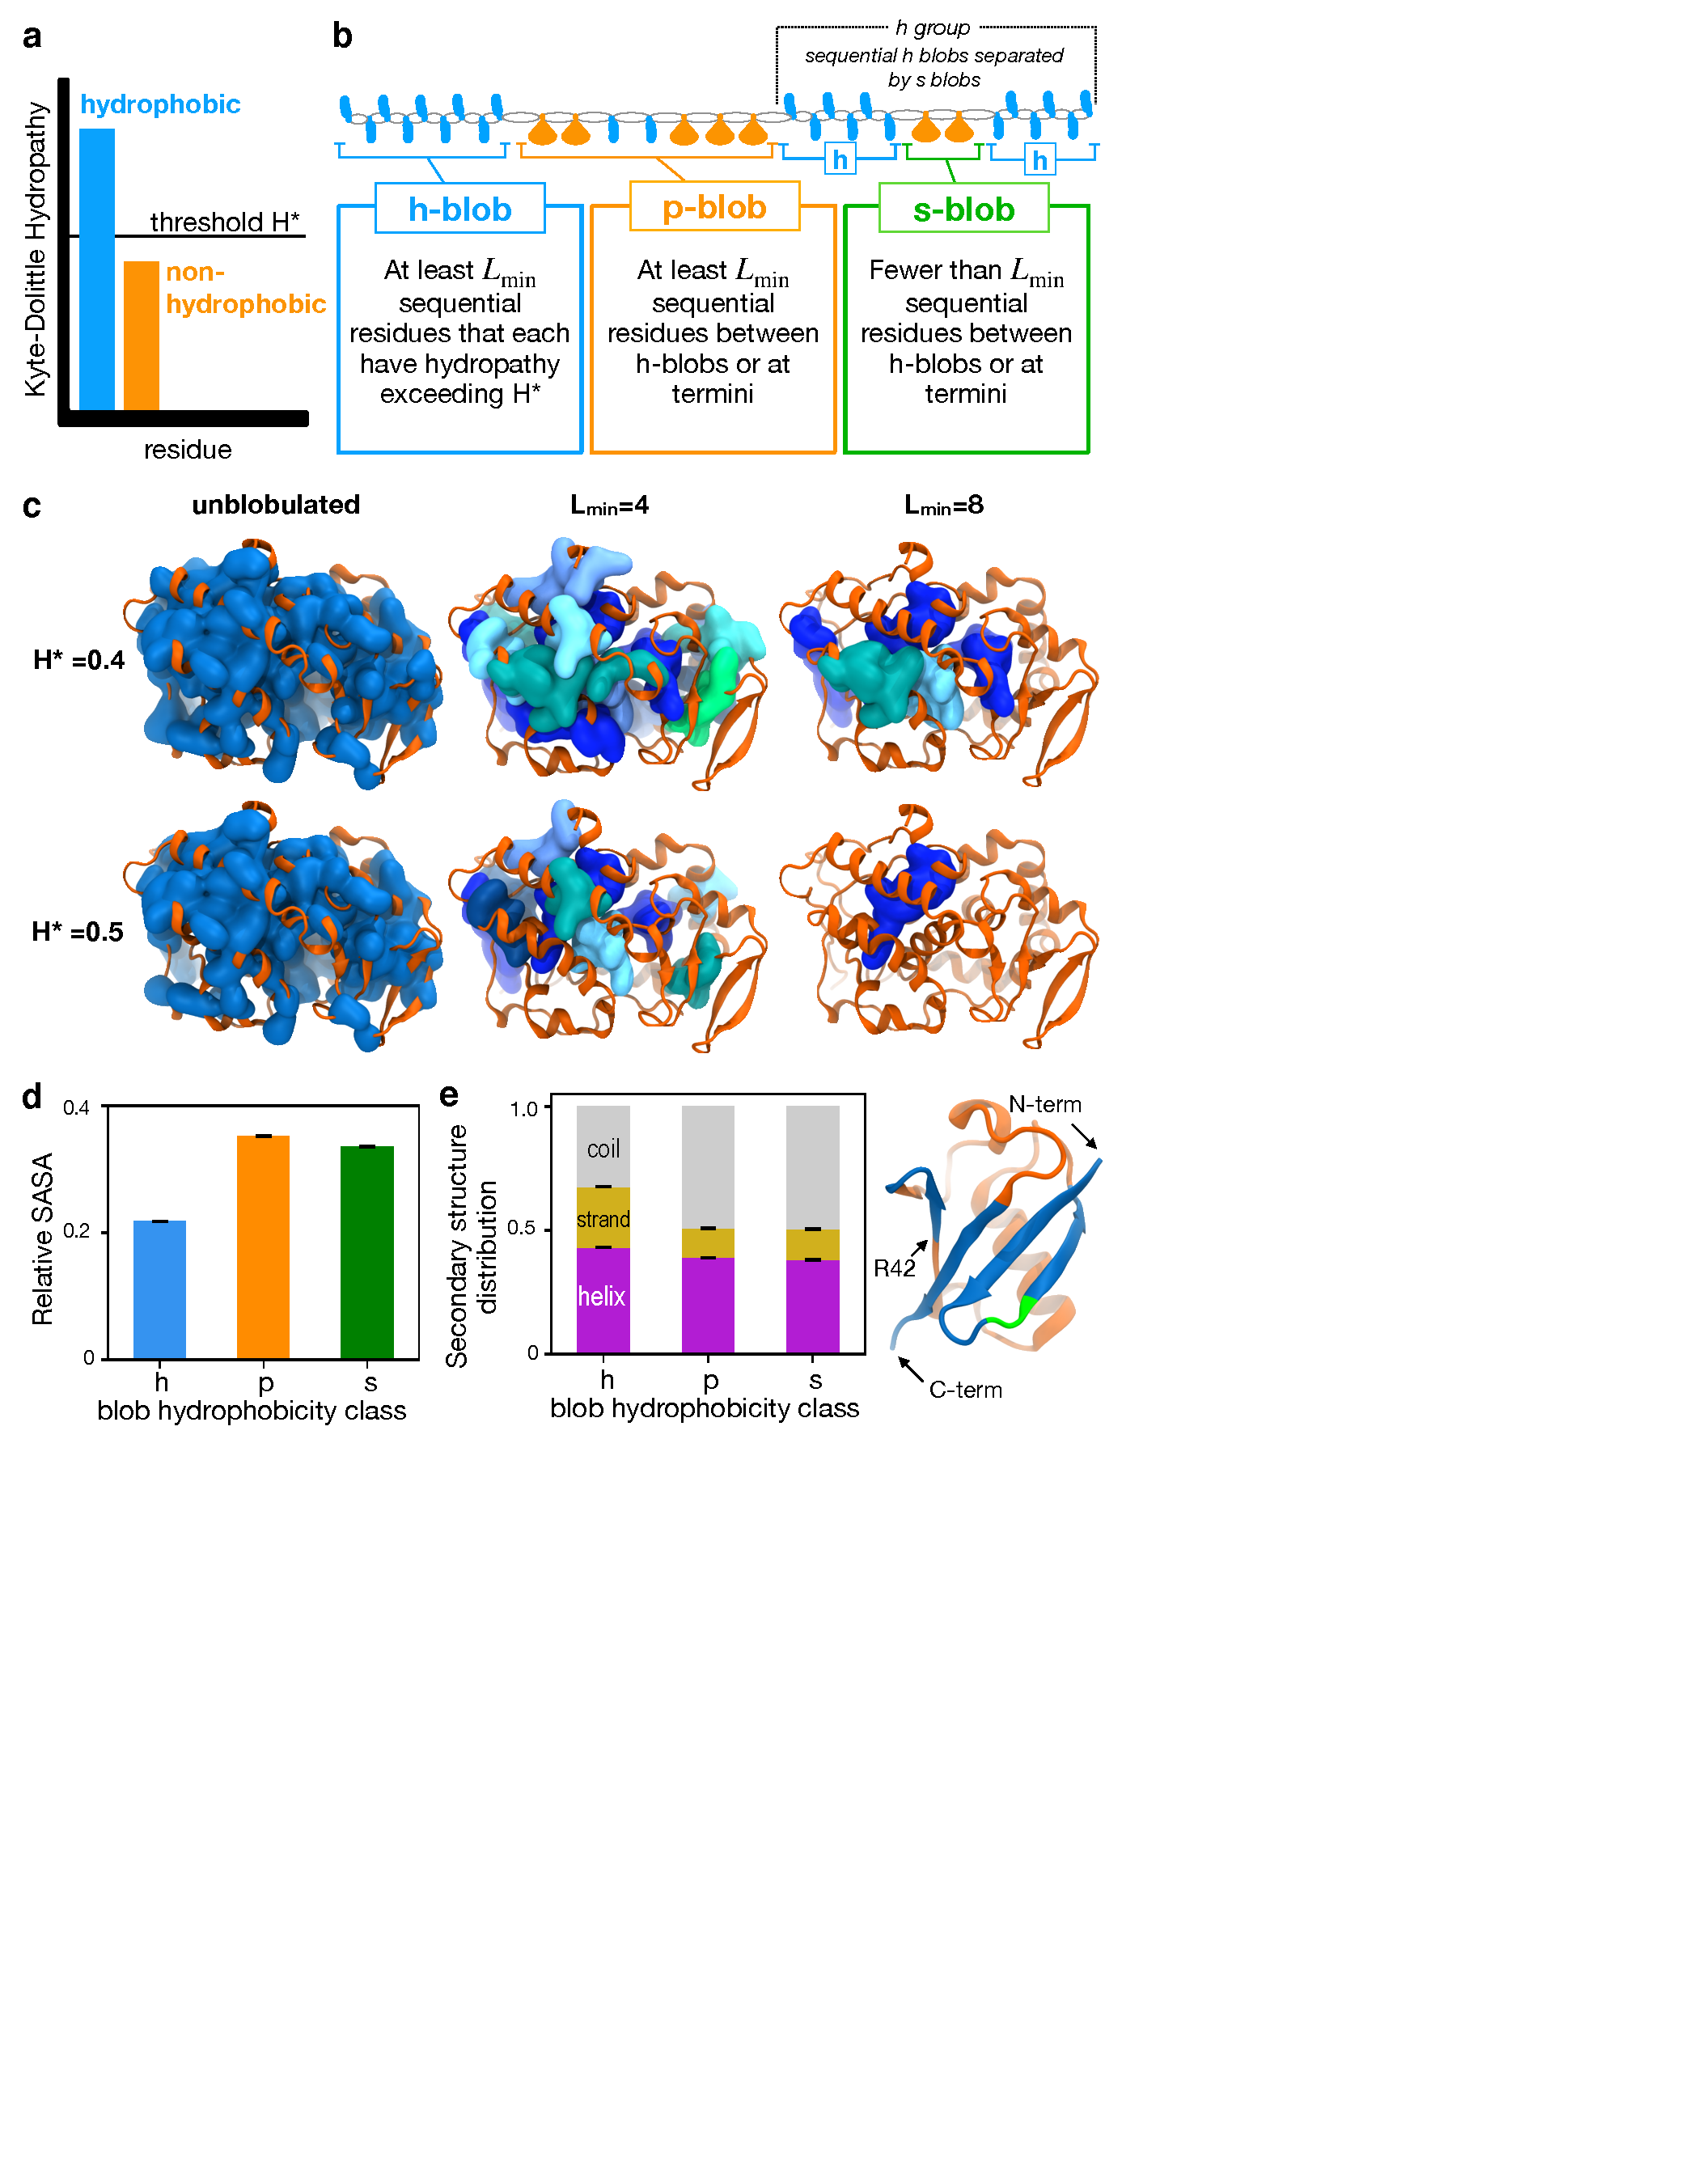
\includegraphics[scale=1,width=\textwidth,trim={0 0cm 0 0cm},clip]{./figures/fig1.pdf}
%DIFDELCMD < %%%
%DIFDELCMD < \caption{%
{%DIFAUXCMD
%DIFDELCMD < {\bf %%%
\DIFdelFL{Cartoon representation of the blobulation approach.}%DIFDELCMD < } %%%
\DIFdelFL{Left: A given protein chain consists of amino acids that are either hydrophobic (blue ovals) or not hydrophobic (orange fans).  Clusters of hydrophobic residues (gray shading) are likely to be buried and have a high number of interacting residues. Any curve drawn through such a cluster, including the curve representing the peptide chain, will contain contiguous hydrophobic residues. Center: The blobulation algorithm calculates the smoothed hydrophobicity for each residue, and then identifies stretches of at least $\Lmin$ residues above the hydrophobicity threshold (black line), where $\Lmin = 4$ unless otherwise noted.  This process defines the boundaries between blobs, and also provides information about the blob \hydrochar{}: blobs of contiguous hydrophobic residues are ``h" blobs (at least $\Lmin$ residues), while remaining stretches are either p ``blobs" (at least $\Lmin$ residues) and ``s blobs" (fewer than $\Lmin$ residues). Right: Blobs mapped onto the peptide chain; the peptide backbone is colored according to blob \hydrochar{} and black circles mark the boundary between blobs. In this illustration there are 4 h-blobs, 2 p-blobs, and 1 s-blob.}}
%DIFAUXCMD
\DIFdelendFL \DIFaddbeginFL \begin{figure}
%DIF > \centering
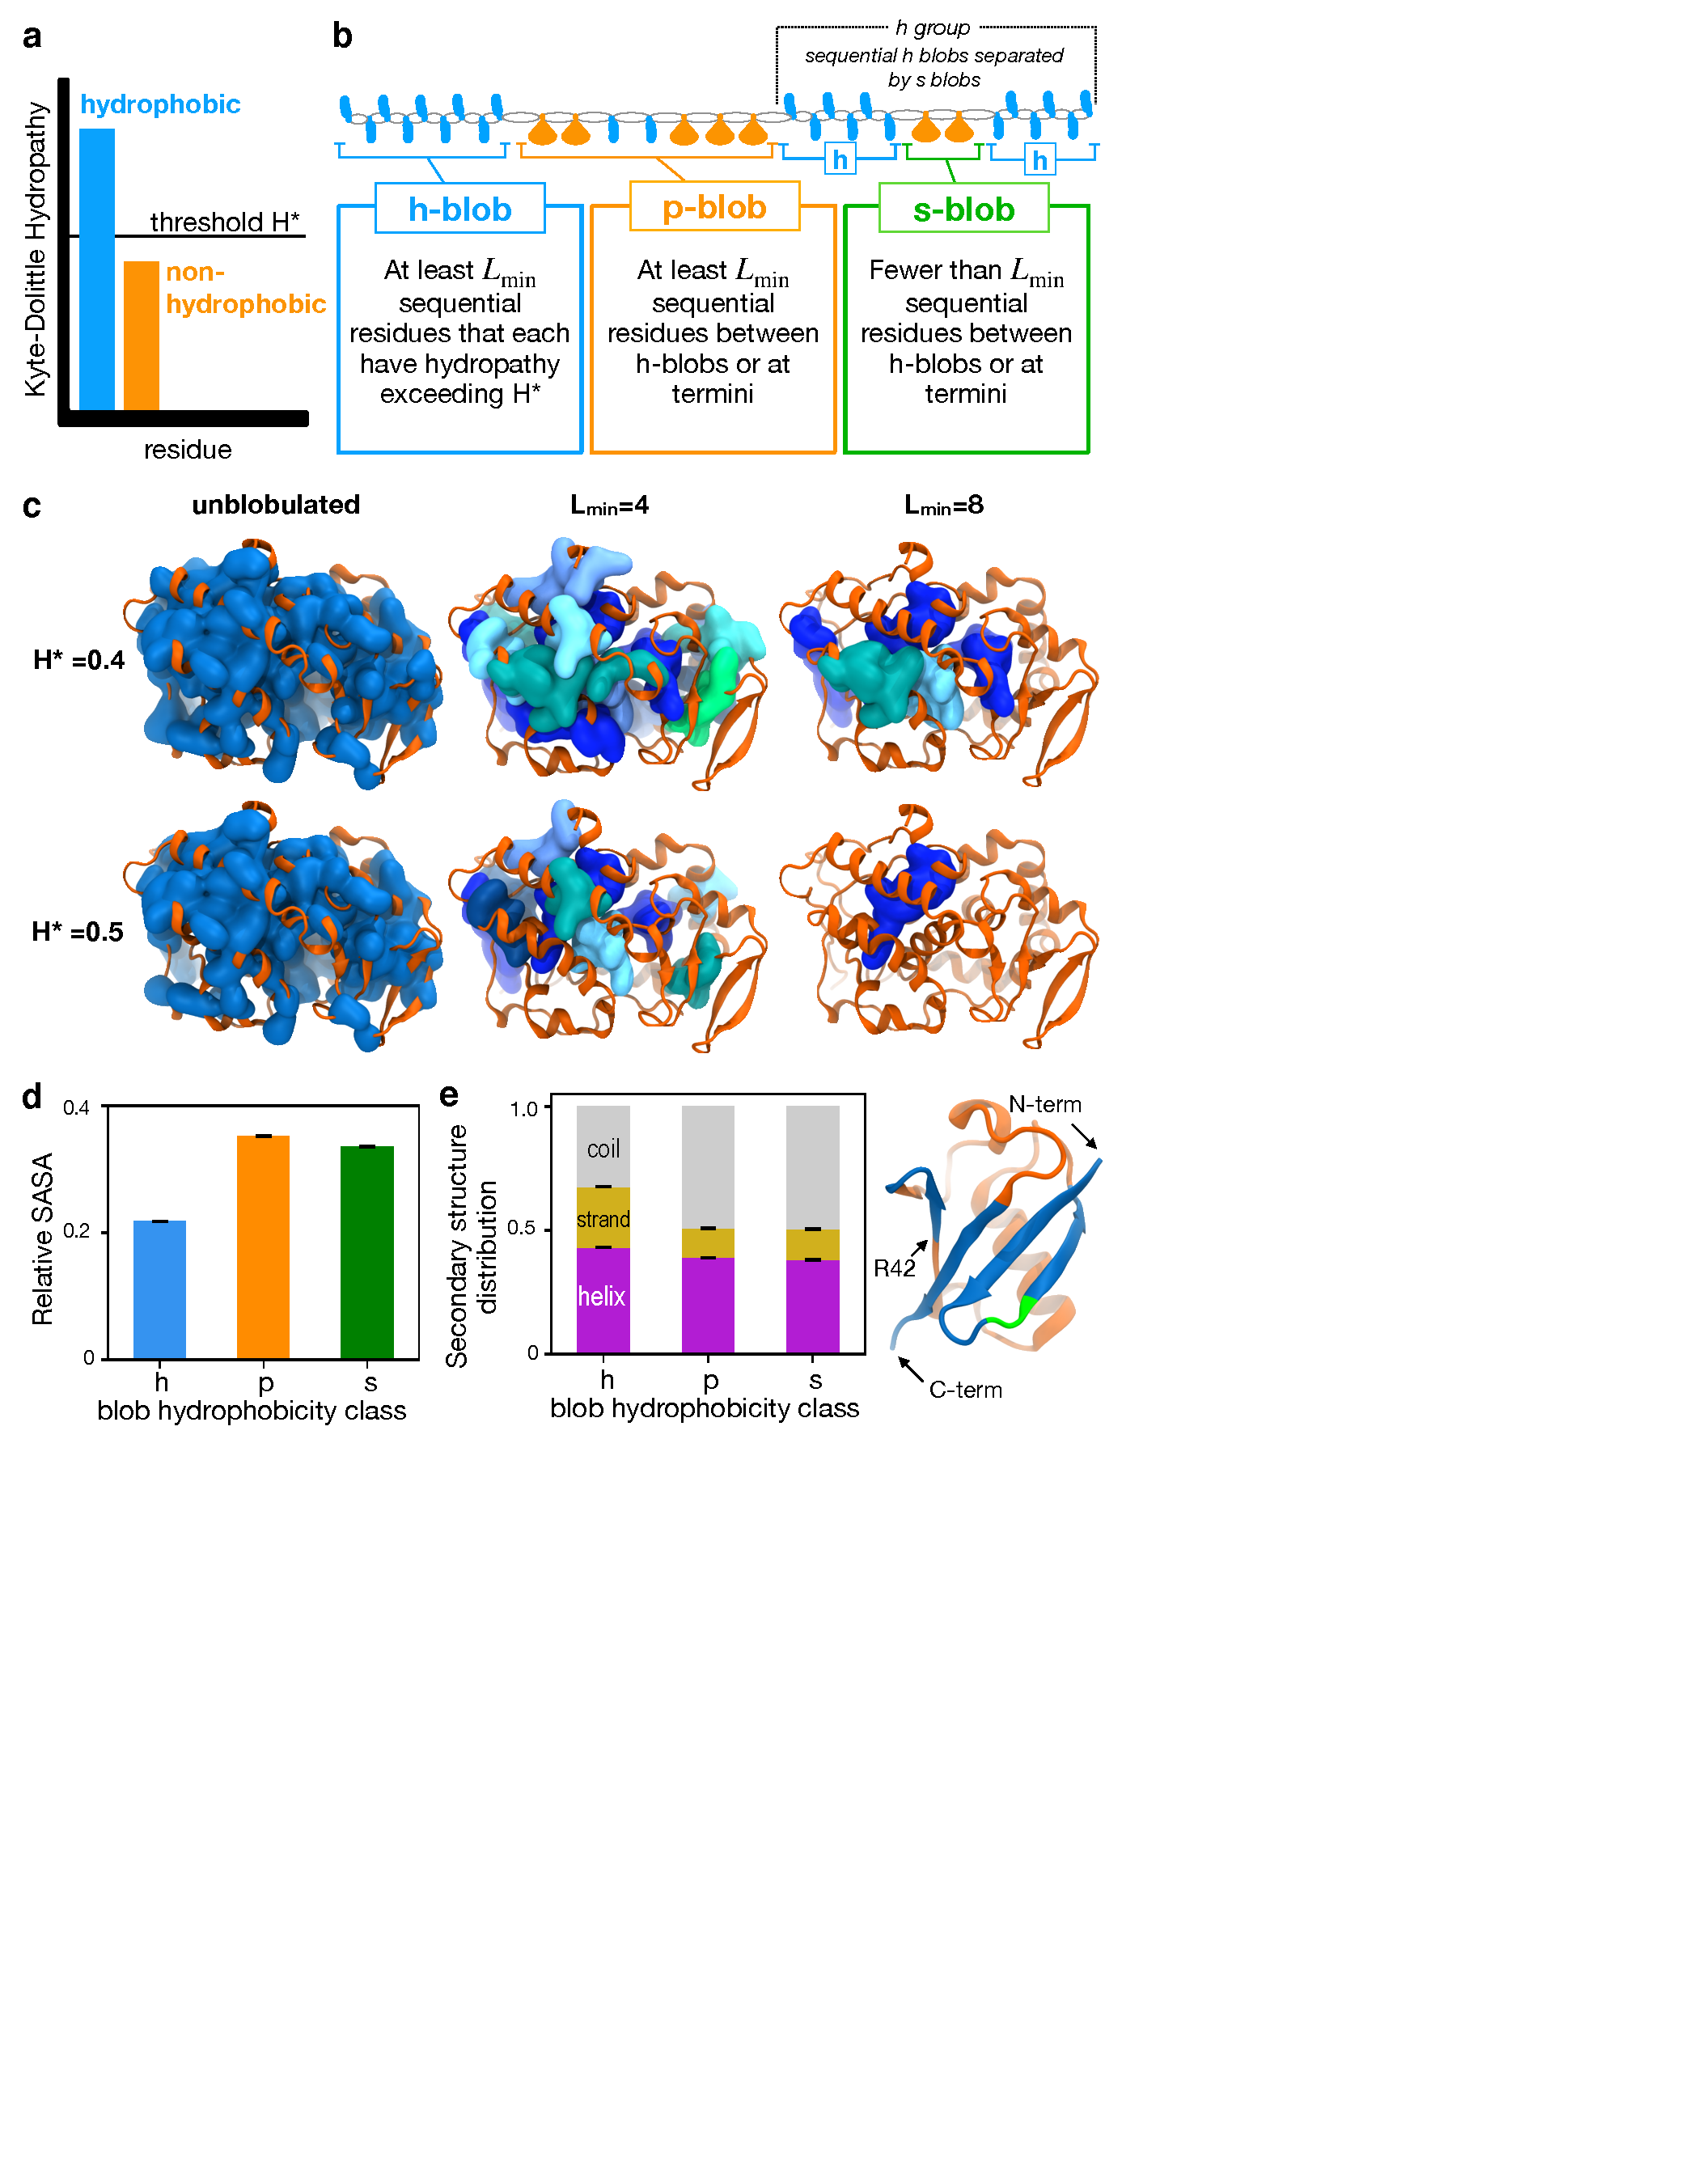
\includegraphics[width=0.5\textwidth]{./figures/fig1.pdf}
\caption{{\bf \DIFaddFL{Whole-sequence blobulation algorithm for segmentation of proteins.}} \DIFaddFL{a) First, the sequence is digitized: residues are classified as hydrophobic or non-hydrophobic depending on whether they have a Kyte-Dolittle \mbox{%DIFAUXCMD
\cite{Kyte1982} }\hspace{0pt}%DIFAUXCMD
hydropathy falling above or below the user-provided threshold $\Ht$, respectively. b) The clustering step acts on the digitized sequence, which is illustrated here as a cartoon: residues above and below the $\Ht$ threshold are shown as blue ovals and orange fans respectively. The clustering step scans the digitized sequence according to the indicated criteria, first detecting h-blobs, then p-blobs, and finally s-blobs. $\Lmin$ is the user-provided minimum blob size. The blobulation outcome for this particular chain would be valid for $2<\Lmin<6$. The software and a web-interface are freely available as described in Methods. c) Cytochrome C peroxidase (2CYP\mbox{%DIFAUXCMD
\cite{Finzel1984}}\hspace{0pt}%DIFAUXCMD
) shown for two different digitization thresholds $\Ht$ (rows), and three different clustering criteria (columns), including no clustering (left ``unblobulated'' column) or two different values of $\Lmin$ (middle and right column, respectively).  The blue surface of the unblobulated sequence depicts canonical hydrophobic residues; the $\Ht=0.4$ row also includes Serine and Threonine, which have Kyte-Dolittle hydropathy scores of 0.41 and 0.42 respectively. H-blobs in the middle and right columns are colored by arbitrarily varying shades of blue to distinguish individual blobs. d) Relative solvent-accessible surface area (SASA) for non-transmembrane blobs in the Protein Data Bank (PDB), categorized by blob hydrophobicity class. e) Left: Distribution of secondary structures for sequences with structures in the PDB, categorized by blob hydrophobicity class. Right: Blobulated ubiquitin (PDBID 5GO7\mbox{%DIFAUXCMD
\cite{Gao2016}}\hspace{0pt}%DIFAUXCMD
), colored by blob hydrophobicity class, as in B. In both panels d and e, the blobulation algorithm uses $\Lmin=4$ and $\Ht=0.4$; error bars are standard errors as described in Methods and Materials ($n>500,000$ for h- and p-blobs, $n>50,000$ for s- blobs). }}
\DIFaddendFL \label{cartoon} 
\end{figure}
}\fi

\DIFaddbegin \DIFadd{The blobulation algorithm, first presented in Ref. \mbox{%DIFAUXCMD
\cite{Lohia2019}}\hspace{0pt}%DIFAUXCMD
, is a method for tunable segmentation or edge detection in protein sequences based on hydrophobicity. The original ``whole-sequence'' blobulation algorithm digitizes the sequence and then clusters it. In the preliminary digitization step (Figure \ref{cartoon}A), each residue is classified as hydrophobic or non-hydrophobic, depending on whether the Kyte-Dolittle hydropathy score\mbox{%DIFAUXCMD
\cite{Kyte1982} }\hspace{0pt}%DIFAUXCMD
is above or below the hydrophobicity threshold $\Ht$. In the main clustering step (Figure \ref{cartoon}B),  the algorithm scans the given amino acid sequence to identify stretches of at least $\Lmin$ sequential residues that were classified as hydrophobic during digitization. These stretches are called hydrophobic blobs or ``h-blobs''. 
}

\DIFadd{The residues that are not assigned to h-blobs will contain a mix of non-hydrophobic residues and isolated hydrophobic residues, in stretches that either link h-blobs or terminate the sequence: short stretches that contain fewer than $\Lmin$ residues are classified as separator or ``s-blobs'', while long stretches with at least $\Lmin$ residues are classified as polar or ``p-blobs.'' The blobs can then be characterized based on any collective property of the blob sequence; the h, p, and s designation also constitute the primary blob characterization termed the ``\hydrochar''. In Ref. \mbox{%DIFAUXCMD
\cite{Lohia2019} }\hspace{0pt}%DIFAUXCMD
we also introduced a higher order classification: adjacent h-blobs that were separated only by the short s-blobs were called ``h-groups''. We include this designation in Figure \ref{cartoon}B for completeness but do not explicitly consider h-groups in this paper. However, h-groups }\emph{\DIFadd{are}} \DIFadd{captured implicitly by variation of the $\Ht$ threshold; the long h-blobs that are detected at low $\Ht$ would be classified as h-groups at high $\Ht$. %DIF > Given the two parameters $\{\Ht,\Lmin\}$, any amino acid sequence can be unambiguously and completely decomposed into a series of h, p,and s- blobs.
}

\DIFadd{The blobulation algorithm can be used in multiple ways, and we apply it in three slightly different ways within this study. In the original ``whole sequence'' version just described, the entire sequence is unambiguously and completely decomposed into h-, p-, and s-blobs using two fixed parameters $\{\Ht,\Lmin\}$ provided by the user.  }\DIFaddend In \DIFaddbegin \DIFadd{this section we will continue to use this approach, because the analysis considers whole proteins. Alternatively, we can fix one residue and one parameter, and calculate or optimize the second parameter. In subsequent sections we will use two such variations (``unconstrained length'' and ``unconstrained threshold'') for analyzing the blob properties surrounding specific sets of SNPs. Both approaches are described further at first use. 
}

\DIFadd{We find that nearly half of the residues in the proteome meet our original\mbox{%DIFAUXCMD
\cite{Lohia2019} }\hspace{0pt}%DIFAUXCMD
relaxed criteria for h-blobs, which includes short, moderately hydrophobic sequences. More specifically, using $\Lmin=4$ and $\Ht=0.4$, the residues in the UniProt dataset (N = 6,594 proteins) are distributed as follows: 45\% in h-blobs, 52\% in p-blobs, and 3\% in s-blobs. Stricter criteria can be used to isolate the long, highly hydrophobic blobs that cover less than 10\% of the proteome: using $\Ht=0.5$ and $\Lmin=8$, the distribution is 7\% in h-blobs, 93\% in p-blobs, and $<1$\% in s-blobs. The effect of varying these two parameters is shown for cytochrome C peroxidase in Figure \ref{cartoon}C; as the criteria is made more restrictive, the algorithm isolates one long and very hydrophobic blob at the core of the protein.
}

\DIFadd{To test the hypothesis that h-blobs would be buried in globular, structured proteins, we calculated the relative solvent-accessibility surface area (SASA) for each blob type, determined using structures in the Protein Data Bank (PDB) (excluding transmembrane domains). Relaxed criteria ($\Lmin=4, \Ht=0.4$) were used for this calculation to maximize the amount of available data and to keep the analysis conservative.  These calculations (Figure \ref{cartoon}D) confirmed that residues in h-blobs have a substantially lower SASA (0.21) than p-blobs (0.35) or s-blobs (0.33); standard error for all three quantities is less than 0.001. Together, these results suggest that h-blobs condense into buried clusters that are rich in intra- or inter-protein interactions. As illustrated in Figure \ref{cartoon}C, we expect this difference to be even larger for h-blobs that meet stricter criteria.
}

\DIFadd{The overlap between blob \hydrochar{} and secondary structure was measured by blobulating all unique proteins in the PDB and tabulating the fraction of residues occurring in helices ($\alpha$, 3-10, $\pi$), strand ($\beta$-bridge or extended $\beta$ strand), or coil for each blob type. 
As shown in Figure \ref{cartoon}E, all blob types contain a comparable fraction of helices, although the fraction in h-blobs is slightly greater than in non h-blobs. We do not expect contiguous hydrophobicity to be particularly correlated with helical structure (with the exception of transmembrane helices): helices frequently have multiple faces with differential solvent accessibility, and the sequence needs to cycle through residues that are appropriate for each face. H-blobs, however, are about twice as likely to contain strands as non h-blobs (Figure \ref{cartoon}E). $\beta$-strands are secondary structure elements, but they are also indicators of tertiary interactions, since $\beta$-strands will have a pairing $\beta$-strand. These results are consistent with our first application of blobulation to simulated conformations of the long disordered pro region of BDNF\mbox{%DIFAUXCMD
\cite{Lohia2019}}\hspace{0pt}%DIFAUXCMD
, which revealed a network of soft tertiary interactions mediated through pairing of $\beta$ strands in h-blobs. 
}

\DIFadd{As an example, Figure \ref{cartoon}E also shows the blob assignments for the ubiquitin sequence mapped onto its structure. The N-terminal $\beta$-hairpin is assigned to two h-blobs, separated by an s-blob that is adjacent to the turn. The C-terminal $\beta$-strand is also assigned to an h-blob, capped by an s-blob at the terminus. Finally, the Pro37-Ala46 $\beta$-strand is a p-blob from Pro37 to Arg42 and then switches to an h-blob as it crosses into the h-blob rich part of the protein. That h-blob continues until the chain bends back toward the other p-blobs. This example suggests that while blob boundaries can align with secondary structure elements, they are more fundamentally correlated with the location of the blob within the three-dimensional protein structure. 
}

\subsection*{\DIFadd{Average local hydrophobicity is a weak indicator of disease-association}}
\DIFadd{In }\DIFaddend order to test whether the \DIFdelbegin \DIFdel{hydrophobicity of a reference allele was correlated with its }\DIFdelend \DIFaddbegin \DIFadd{residue hydrophobicity is }{\em \DIFadd{prima facie}} \DIFadd{correlated with }\DIFaddend functional impact, we calculated the enrichment of \DIFdelbegin \DIFdel{\dSNPs relative to \nSNPs }\DIFdelend \DIFaddbegin \DIFadd{disease-associated SNPs (dSNPs) }\DIFaddend as a function of hydrophobicity of the reference allele \DIFdelbegin \DIFdel{.  }\DIFdelend \DIFaddbegin \DIFadd{(see Materials and Methods and SI Dataset 1). Throughout this paper, unless otherwise noted, \dSNPs are tested for enrichment relative to the expectation set by SNPs that are not disease-associated (nSNPs). For example, the phrase ``\dSNPs are enriched in blobs of type X'' means that the proportion of \dSNPs found in blobs of type X is larger than the proportion of \nSNPs found in blobs of type X. }\DIFaddend As shown in Figure \ref{blob_vs_window}\DIFdelbegin \DIFdel{b}\DIFdelend \DIFaddbegin \DIFadd{B}\DIFaddend , we did not detect any significant correlation (Pearson's r=0.02, n=17) \DIFdelbegin \DIFdel{.  Hydrophobicity is a highly cooperative phenomenon \mbox{%DIFAUXCMD
\citep{Jiang2017}}\hspace{0pt}%DIFAUXCMD
, and we hypothesized }\DIFdelend \DIFaddbegin \DIFadd{between lone SNP hydrophobicity and dSNP enrichment, meaning }\DIFaddend that the hydrophobicity of \DIFdelbegin \DIFdel{the local sequence could be critical for determining the functional effects of the \dSNP. We considered two methods for determining local sequence context: our own ``blobulation" approach and a fixed-width moving window . 
}\DIFdelend \DIFaddbegin \DIFadd{a residue considered in isolation does not show this particular signature of functionality.
}\DIFaddend 

\DIFdelbegin \DIFdel{Blobulation (Figure \ref{cartoon})is a particular systematic approach for identifying modular components in the protein sequence, which we previously introduced \mbox{%DIFAUXCMD
\citep{Lohia2019} }\hspace{0pt}%DIFAUXCMD
for analysis of a specific protein }\DIFdelend \DIFaddbegin \DIFadd{The effect of average local hydrophobicity on the enrichment of dSNPs was calculated using moving windows of length $\Lw$ centered around each SNP. 
%DIF > In order to test the effect of average local hydrophobicity on enrichment of dSNPs, we determined the local sequences using a classic moving window of length $L_{\rm w}$, centered around the SNP.  
While there is no ``standard'' window size, most SNP prediction programs use a window size in the range of 1-21 residues~\mbox{%DIFAUXCMD
\citep{Teng2010, Capriotti2006, Capriotti2017, Hecht2015}}\hspace{0pt}%DIFAUXCMD
. The window size is chosen to balance concerns that small window sizes may not accurately capture the ``local'' sequence~\mbox{%DIFAUXCMD
\citep{Chen2006, Schlessinger2005, Sander2006} }\hspace{0pt}%DIFAUXCMD
whereas long window sizes can decrease signal to noise ratio~\mbox{%DIFAUXCMD
\citep{Park2007}}\hspace{0pt}%DIFAUXCMD
.  Here we computed the mean window hydrophobicity $\bar{H}_i$ for all SNPs $i$ in our SNP dataset, while also varying $\Lw$. Figure \ref{blob_vs_window}C shows the enrichment of \dSNPs for which $\bar{H}_i > \Ht$, for the range of moving window widths $\Lw=1-99$. As is evident in Figure \ref{blob_vs_window}C, the enrichment of \dSNPs is relatively insensitive to the window size for the regime where $\Lw \ge 6$ and $\Ht \le 0.65$. The total count of \nSNPs in each bin is shown in Fig ~\ref{blob_vs_window}G, and was similarly insensitive to window size for larger thresholds. These results suggest that distant residues introduce noise that averages out in a proteome-wide analysis, but their inclusion in the window would still reduce precision for any individual SNP}\DIFaddend . 
\DIFdelbegin \DIFdel{Here we have generalized and extended the approach by varying two previously-fixed parameters (minimum blob length and hydrophobicity threshold) that are required to define blob edges, as described in }\DIFdelend \DIFaddbegin 

\DIFadd{Surprisingly, we detect a narrow band of \dSNP depletion for windows with a high average hydrophobicity (the red signal for $\Ht\ge 0.65$ in Figure \ref{blob_vs_window}C). This signal is due to only a handful of SNPs (see the counts in Figure \ref{blob_vs_window}G), but we observe a similar pattern using the blobulation algorithm, and we discuss its origins in the next sections.
}

\ifnum\value{\DIFadd{includefigs}}\DIFadd{>0 }\DIFaddend {
\DIFdelbegin %DIFDELCMD < \it %%%
\DIFdel{Methods}\DIFdelend \DIFaddbegin \begin{figure*}
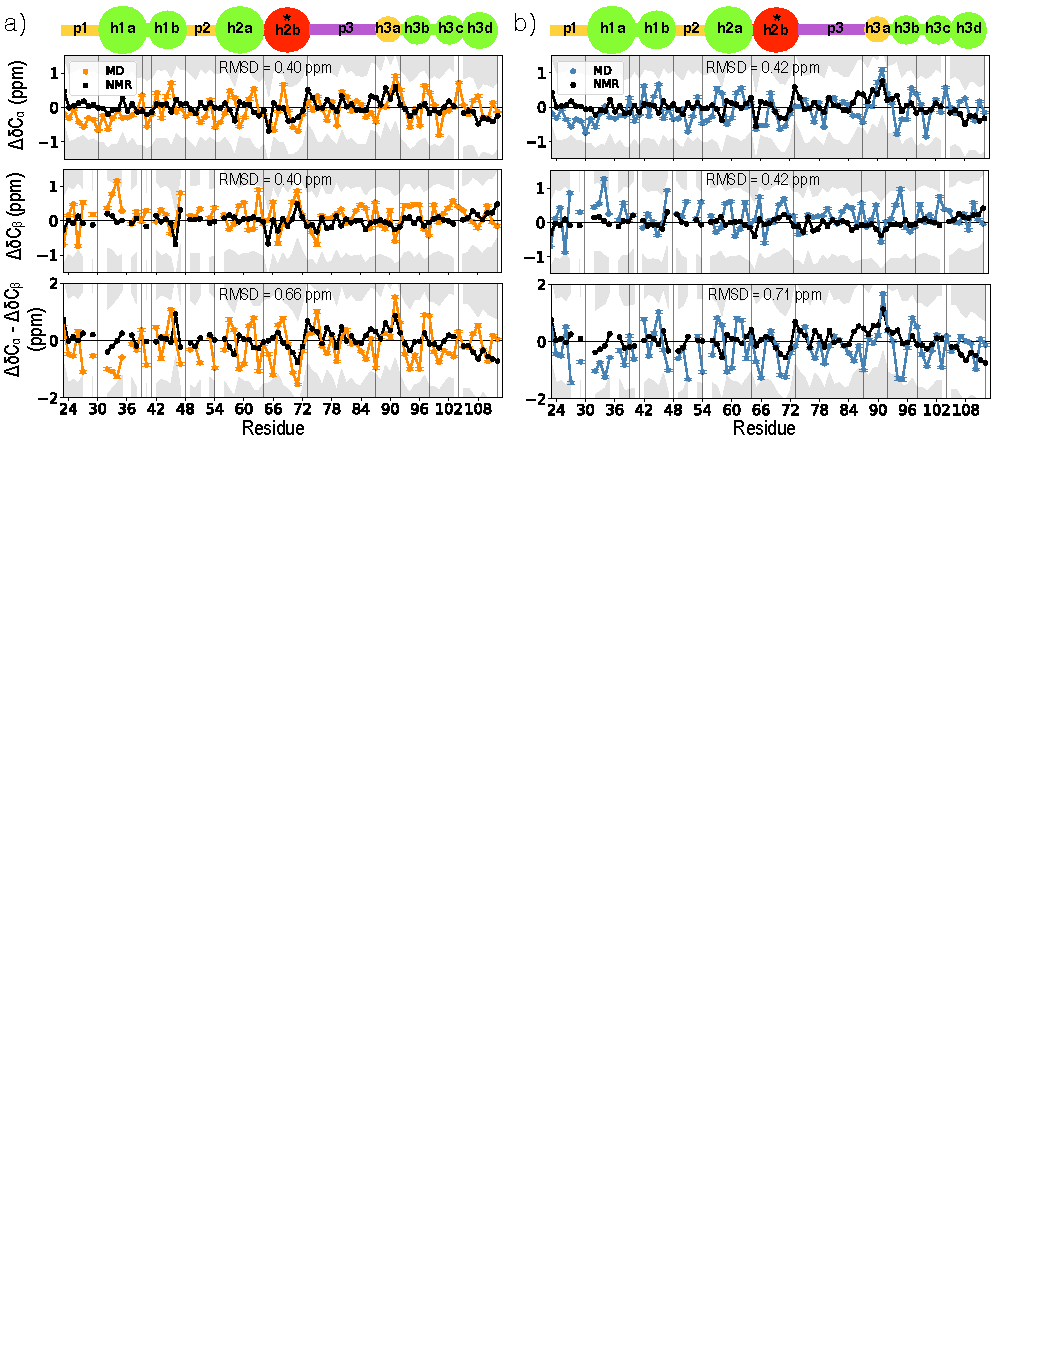
\includegraphics[scale=1,width=\textwidth,trim={0 0cm 0 0cm},clip]{./figures/fig2.pdf}
\caption{{\bf \DIFaddFL{Effect of segmentation approach, length,  hydrophobicity threshold, and environment on calculated enrichment of \dSNPs in hydrophobic segments.}} \DIFaddFL{a) Illustration of three measures of SNP hydrophobicity (residue, contiguous, and average local) for the indicated SNP, found within a hypothetical peptide chain composed of residues classified as hydrophobic (blue ovals) or non-hydrophobic (orange fans) for a given $\Ht$, as in Figure \ref{cartoon}B. Unconstrained-length blobulation determines the local sequence (shaded in gray) by detecting contiguous hydrophobic residues, which together form an h-blob of length $L$; the moving window approach determines the local sequence using a fixed number $L_w$ of residues centered around the SNP. b) Enrichment of disease-associate SNPs (dSNPs) relative to non disease-associated SNPs (nSNPs) as a function of hydrophobicity of the reference allele, with line of best fit. No trend or significant correlation is observed (Pearson's r=0.02, p=0.94, n=17). (c-f) Enrichment of \dSNPs in hydrophobic segments, as a function of segment length and threshold, for (c) fixed-length hydrophobic windows of length $L_w$ in which the average hydrophobicity is above $\Ht$, or (d-f) h-blobs of length $L$, calculated with the threshold $\Ht$ for (h) all SNPs, (i) those outside of transmembrane domains or (j) those in transmembrane domains.  g-j) The total number of \nSNPs in (g) windows of length $L_w$ for which the average hydrophobicity is above $\Ht$, or (h-i) h-blobs of length $L$, calculated with the threshold $\Ht$ for (h) all SNPs, (i) those outside of transmembrane domains or (j) those in transmembrane domains. Each panel (c-j) is colored according to the scale at the right end of the row, and bins with no data are colored gray.}}
\label{blob_vs_window} 
\end{figure*}
\DIFaddend }\DIFdelbegin \DIFdel{. The degree of enrichment for disease-association is expected to be dependent upon both of these parameters, and we ran enrichment tests for a wide range of minimum blob lengths and hydrophobicity }\DIFdelend \DIFaddbegin \fi 
\subsection*{\DIFadd{Contiguous hydrophobicity is a strong indicator of disease-association}}

\DIFadd{The use of a fixed-width window neglects the inherent dispersion in the size of protein modules, which are captured using blobulation (Figure \ref{blob_vs_window} A). To quantify the blob properties for each SNP, we used a blobulation variant we call ``unconstrained length'' blobulation, which fixes the }\DIFaddend threshold \DIFdelbegin \DIFdel{values.  Unless otherwise noted, \dSNPs are tested for enrichment relative to the expectation set by \nSNPs. For example, }\DIFdelend \DIFaddbegin \DIFadd{$\Ht$ and a reference residue $i$ but imposes no minimum blob length. This approach first tests whether the hydropathy score for residue $i$ exceeds $\Ht$, and if so, it calculates the exact length $L$ of }\DIFaddend the \DIFdelbegin \DIFdel{phrase ``\dSNPs are enriched in X blobs" means that \dSNPs are found at a higher rate in blobs of type X than are \nSNPs . 
}%DIFDELCMD < 

%DIFDELCMD < %%%
\DIFdel{We found a consistent trend relating }\DIFdelend \DIFaddbegin \DIFadd{h-blob that contains residue $i$. ``Unconstrained length'' blobulation is formally equivalent to ``whole-sequence'' blobulation with $\Lmin=1$, but is more efficient since we are only analyzing the relevant part of the sequence. 
}

\DIFadd{Specifically, we applied unconstrained-length blobulation to each SNP in the dataset (using the reference allele) and a given hydrophobicity threshold $\Ht$, and then determined $L$.  We repeated this calculation for a series of $\Ht$ values, and for dSNPs and nSNPs separately (SI Dataset 1), and then tabulated the proportion of dSNPs and nSNPs in each $(\Ht,L)$ bin. The resulting enrichment of \dSNPs as a function of blob length $L$ and threshold $\Ht$ is shown in Figure \ref{blob_vs_window}D, and the total number of \nSNPs per bin shown in Figure \ref{blob_vs_window}H (SI Dataset 2).
%DIF > 
%DIF > We note that blobulation can be used in several different ways: given a protein and thresholds $\{\Ht,\Lmin\}$ we can blobulate the sequence into h, p, and s domains, or given a residue and $\Ht$ we can compute the type of blob it lies within and it's size (blob length), or given a residue and $\Lmin$ we can compute the largest hydrophobicity threshold for which it resides in an h-blob. The second approach is formally equivalent to blobulating the entire proteome with $\Lmin=1$ (allowing for all h-blob lengths) and then inspecting only the residues of interest. We use this approach to determine the enrichment of \dSNPs as a function of blob length and threshold $\Ht$ (Figure \ref{blob_vs_window}D), with the total number of \nSNPs per bin shown in Figure \ref{blob_vs_window}H. 
%DIF > 
We observe a consistent relationship between }\DIFaddend hydrophobicity of the local blob and \DIFdelbegin \DIFdel{enrichment of disease-associated SNPs (Figure \ref{blob_vs_window} C)}\DIFdelend \DIFaddbegin \DIFadd{\dSNP enrichment}\DIFaddend .  \dSNPs are depleted in weakly hydrophobic blobs, neutral for moderately hydrophobic blobs, and become more enriched as the blob gets longer and/or satisfies a stricter hydrophobicity threshold. %DIF <  overall magnitudes of the enrichment is  found for blobs that have a contiguous stretch of at least 23 residues with hydrophobicity greater than 0.5; more than three times as many \dSNPs than \nSNPs are located in such blobs. 
The trend is steadily monotonic, which supports the hypothesis that hydrophobic blobs constitute identifiable functional elements.
\DIFdelbegin \DIFdel{The exception is }\DIFdelend \DIFaddbegin 

\DIFadd{We do find an exception to the trend }\DIFaddend at the plot boundary: \DIFdelbegin \DIFdel{surprisingly, }\DIFdelend blobs that satisfied the very strictest criteria were depleted in \DIFdelbegin \DIFdel{\dSNPs. }\DIFdelend \DIFaddbegin \DIFadd{dSNPs, consistent with the results using the moving window analysis. The depletion signal persisted even when bins with very few blobs were removed. }\DIFaddend In the next section, we consider two potential reasons for this depletion: either \dSNPs in these blobs are so deleterious that they are selected out of the population, or \DIFdelbegin \DIFdel{\nSNPs in these blobs are functional as expected, but not deleterious. %DIF < This continuous trend supports the hypothesis that \hydrochar{} segments constitute identifiable functional elements %and a risk-factor \grace{word choice} for disease-association, and
}\DIFdelend \DIFaddbegin \DIFadd{some subset of \nSNPs are functional and under balancing selection or relaxed constraint. }\DIFaddend In addition to a consistent trend, the analysis returns a large spread in enrichment/depletion values:  3.2\% of the bins in Figure~\ref{blob_vs_window}\DIFdelbegin \DIFdel{c have a significant enrichment of less than }\DIFdelend \DIFaddbegin \DIFadd{D are significantly depleted below }\DIFaddend 0.5, while 13\% have a significant enrichment of greater than 1.5, and 3.5\% have a significant enrichment greater than \DIFdelbegin \DIFdel{3 (Data set 1). This result }\DIFdelend \DIFaddbegin \DIFadd{3. This range }\DIFaddend indicates that hydrophobicity-based sequence segmentation could be particularly useful for assessing the riskiness of SNPs located in long \DIFdelbegin \DIFdel{and }\DIFdelend \DIFaddbegin \DIFadd{or }\DIFaddend very hydrophobic sequences. \DIFaddbegin \DIFadd{To this end, the numerical enrichment values for each bin are provided in Dataset S1.
}\DIFaddend 

\DIFdelbegin \DIFdel{In order to compare the effectiveness of blobulation to a moving window approach, we ran analogous enrichment tests for sliding windows across all protein sequences.
Two analogous parameters (window length and mean hydrophobicity threshold) are used for defining hydrophobic regions in the moving window approach, with the resulting enrichment for a range of these values also shown in Fig~\ref{blob_vs_window}d. Compared to the blobulation approach, }\DIFdelend \DIFaddbegin \DIFadd{Transmembrane helices will intrinsically require contiguous residues that are at least moderately hydrophobic (with the exception of pore-lining helices) and it seemed possible that our results were dominated by the distinctive properties of such transmembrane domains. We further decomposed the data into contributions from SNPs that are not in transmembrane domains (Figure \ref{blob_vs_window}E, SI Dataset 2) and those that are (Figure \ref{blob_vs_window}F, SI Dataset 2). The population counts of \nSNPs for each case are shown in panels (i) and (j) respectively, indicating that the overall dataset includes relatively few SNPs in transmembrane domains. We find that enrichment trends for solvated \dSNPs{} (Figure \ref{blob_vs_window}E) mimic trends in }\DIFaddend the \DIFdelbegin \DIFdel{enrichment detected using the moving window approach is much less sensitive to segment length for windows beyond 6 residues (consider the tilted color bands for the blobulation approach vs the horizontal color bands for moving windows in Figure ~\ref{blob_vs_window}c-d) . The significant depletion in \dSNPs at the most hydrophobic edge is also preserved in the moving window analysis. }%DIFDELCMD < \ifnum%%%
\value{\DIFdel{includefigs}}%DIFAUXCMD
\DIFdel{>0 }%DIFDELCMD < {
%DIFDELCMD < \begin{figure}[!ht]
%DIFDELCMD < 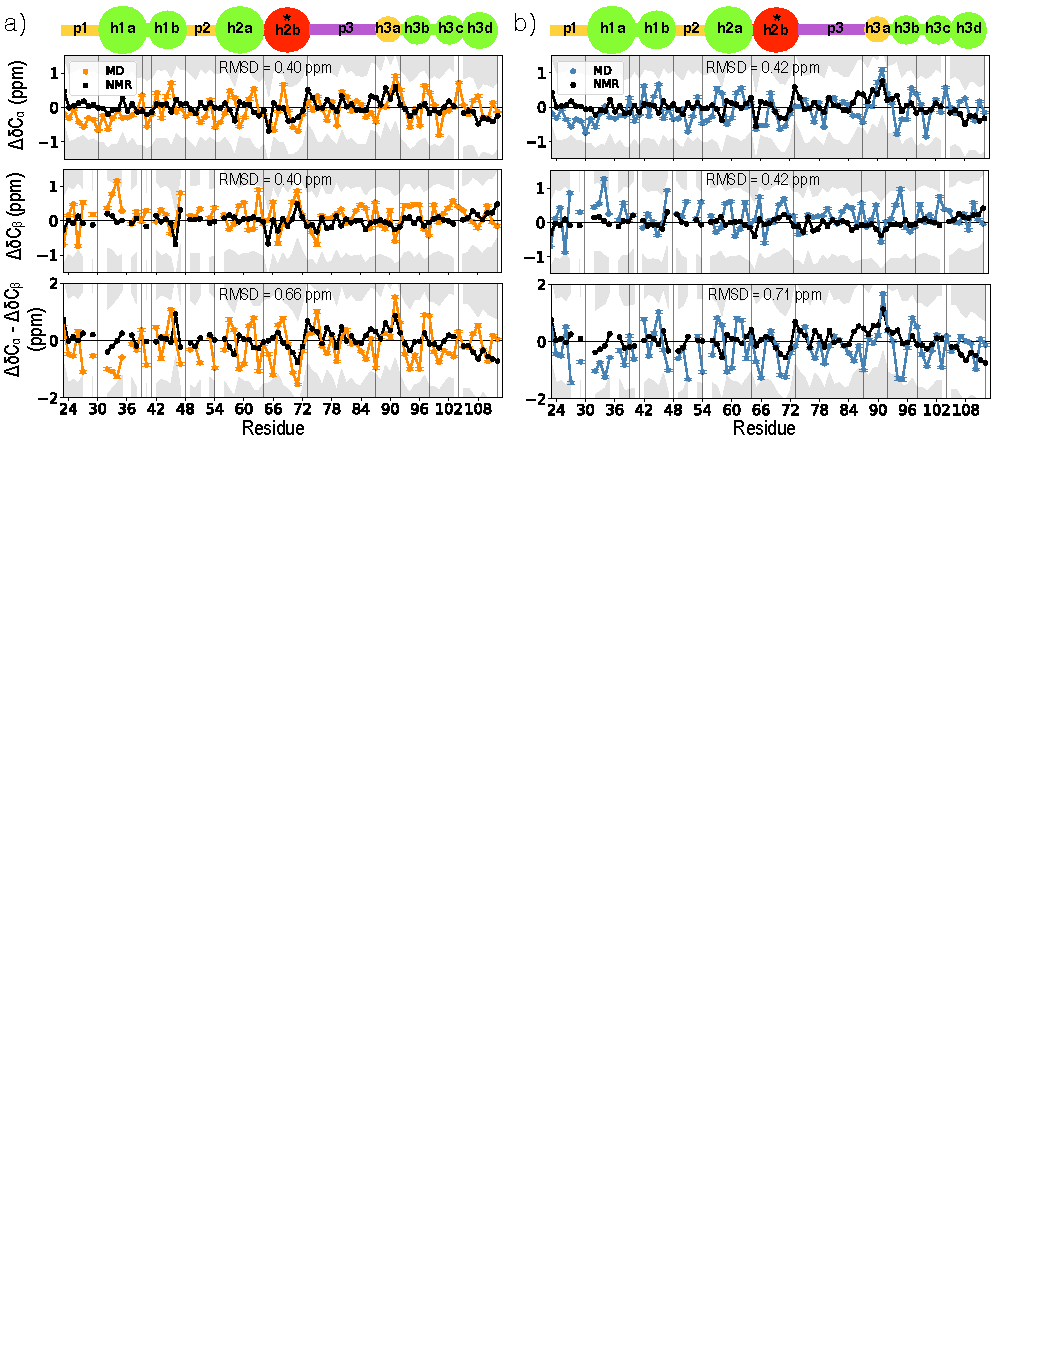
\includegraphics[scale=1,width=1\textwidth,trim={0 0cm 0 0cm},clip]{./figures/fig2.pdf}
%DIFDELCMD < %%%
%DIF < \caption{{\bf Effect of segmentation approach, length, and hydrophobicity threshold on calculated enrichment of \dSNPs in hydrophobic segments.} a) Cartoon of local sequence context for two amino acids (\#1 and \#2) on the hypothetical peptide chain in Figure 1,  as identified using a long moving window (top), blobulation (middle), and a short moving window (bottom). The globular hydrophobic region of Figure 1 is enclosed by the dashed line. Amino acid \#1 lies just inside of an contiguous stretch of hydrophobic amino acids (the dashed boundary line indicates a globular hydrophobic region), while amino acid \#2 lies just outside of a contiguous hydrophobic stretch. Blobulation allows the length of the local sequence to reflect the intrinsic protein properties, specifically the natural hydrophobic segment boundaries.  b) Enrichment of \dSNPs for hydrophobic segments using a blobulation approach (left) and moving window approach (right).  Blobulation defines a hydrophobic segment (or h blob) as a contiguous stretch of a minimum length in which every residue has hydrophobicity greater than the threshold.  In contrast, the moving window approach defines a hydrophobic segment as a stretch of residues of a specific length with a mean hydrophobicity that is greater than the threshold. Each bin is colored according to the fraction of \dSNPs in hydrophobic segments divided by the analogous \nSNP fraction, with the scale shown in the color bar. No data region is shown gray. c) Effect of segmentation parameters on the overall populations of \nSNPs in hydrophobic segments, using the blobulation approach (left) and moving window approach (right). Each bin is colored according to the fraction of \nSNPs that fall in hydrophobic segments.}
%DIFDELCMD < \caption{%
{%DIFAUXCMD
%DIFDELCMD < {\bf %%%
\DIFdelFL{Effect of segmentation approach, length, and hydrophobicity threshold on calculated enrichment of \dSNPs in hydrophobic segments.}%DIFDELCMD < } %%%
\DIFdelFL{a) Illustration of three measures of SNP hydrophobicity (residue, contiguous, and average) for the amino acid shown in purple, found within a hypothetical peptide chain where hydrophobic residues are blue ovals and non-hydrophobic residues are orange fans. The local sequence determined by each segmentation method is shown in black fill. b) Enrichment of \dSNPs relative to \nSNPs as a function of hydrophobicity of the reference allele, with line of best fit. No trend or significant correlation is observed (Pearson's r=0.02, p=0.94, n=17). c-d) Enrichment of \dSNPs relative to \nSNPs for hydrophobic segments for varying hydrophobicity and length thresholds using a blobulation approach (c) and moving window approach (d). 
%DIF < Hydrophobicity thresholds are binned every $0.01$, blob lengths (left) are binned every 1, and window lengths are binned every $2$. 
%DIF < Blobulation defines a hydrophobic segment (or h blob) as a contiguous stretch of a minimum length in which every residue has hydrophobicity greater than the threshold.  In contrast, the moving window approach defines a hydrophobic segment as a stretch of residues of a specific length with a mean hydrophobicity that is greater than the threshold. 
%DIF < Each bin is colored according to the fraction of \dSNPs in hydrophobic segments divided by the analogous \nSNP fraction, with the scale shown in the color bar. 
Bins with no data are shown in gray. e-f) The number of \nSNPs in hydrophobic segments per bin using the blobulation approach (e) and moving window approach (f).}}
%DIFAUXCMD
%DIFDELCMD < \label{blob_vs_window} 
%DIFDELCMD < \end{figure}
%DIFDELCMD < }\fi 
%DIFDELCMD < %%%
\DIFdelend \DIFaddbegin \DIFadd{combined dataset (Figure \ref{blob_vs_window}D). Thus, we conclude that enrichment of \dSNPs{} in h-blobs is a general trend rather than an indication of membrane-exposure.
}\DIFaddend 

\DIFdelbegin \DIFdel{While there is no ``standard" window size, most SNP prediction programs use a window size in the range of 1-21 residues~\mbox{%DIFAUXCMD
\citep{Teng2010, Capriotti2006, Capriotti2017, Hecht2015}}\hspace{0pt}%DIFAUXCMD
.
The window size is chosen to balance concerns that small window sizes may not accurately capture the "local" sequence~\mbox{%DIFAUXCMD
\citep{Chen2006, Schlessinger2005, Sander2006} }\hspace{0pt}%DIFAUXCMD
whereas long window sizes can increase signal to noise ratio~\mbox{%DIFAUXCMD
\citep{Park2007}}\hspace{0pt}%DIFAUXCMD
. In either case, }\DIFdelend \DIFaddbegin \DIFadd{We note that distinguishing between solvated and transmembrane SNPs also suggests appropriate blobulation parameters for transmembrane domains. Transmembrane helices are known to be 24 residues long on average, with about 19 residues forming the hydrophobic core.\mbox{%DIFAUXCMD
\cite{BaezaDelgado2013} }\hspace{0pt}%DIFAUXCMD
As expected, none of }\DIFaddend the \DIFdelbegin \DIFdel{use of a fixed-width window neglects the inherent dispersion in the size of protein modules }\DIFdelend \DIFaddbegin \DIFadd{transmembrane residues are found in h-blobs that are much shorter than 19 residues }\DIFaddend (Figure \ref{blob_vs_window}\DIFdelbegin \DIFdel{a).  The enrichment insensitivity to window size was thus surprising, but the expected noise was likely lost due to averaging across the proteome.  
As shown in Fig ~\ref{blob_vs_window}e, the overall fraction of hydrophobic segments for mild or moderate hydrophobicity thresholds was also insensitive to window size, confirming that the data set we use here is sufficiently large to average out large window noise. For a single SNP, considering too many residues far from the SNP will still contribute significant noise to the prediction.  
}%DIFDELCMD < 

%DIFDELCMD < %%%
\DIFdel{Overall, use of the moving window approach yields two-fold enrichment for only a few, scattered parameter values with very few qualifying sequences}\DIFdelend \DIFaddbegin \DIFadd{J), except when the threshold is sufficiently high to exclude those polar residues that are frequently found in transmembrane helices.  More specifically, raising the threshold beyond $\Ht=0.36$ typically excludes all charged and polar residues but serine and threonine; further raising the threshold beyond $\Ht=0.42$ typically excludes all charged and polar residues. Any transmembrane polar residues that fall below the $\Ht$ threshold will divide the transmembrane into multiple h-blobs, which is consistent with the large number of short h-blobs at high thresholds}\DIFaddend . In contrast, \DIFdelbegin \DIFdel{blobulation yielded greater than two-fold enrichment for a well-defined set of parameters (hydrophobicity threshold $>$ 0.4 and minimum blob size $>$ 15) }\DIFdelend \DIFaddbegin \DIFadd{when short polar and charged linkers between transmembrane segments are included ($\Ht<0.3$) multiple transmembrane segments may be grouped into the same blob, with a minimum length around 20 residues. Such a series of transmembrane segments would also be a common example of the ``h group'' illustrated in Figure \ref{cartoon}B, although we do not use that hierarchical descriptor in this analysis}\DIFaddend .
%DIF < This observation supports our hypothesis that an approach like blobulation, which flexibly defines the local sequence based on natural sequence properties, can provide a more powerful approach for predicting disease association than a moving window approach. 
\DIFdelbegin \DIFdel{This observation supports our hypothesis that blobulation provides a more meaningful and less noisy approach to protein segmentation than use of a fixed-length moving window.
}\DIFdelend 

\subsection*{\DIFdelbegin \DIFdel{Population frequency signatures }\DIFdelend \DIFaddbegin \DIFadd{The genetic diversity }\DIFaddend of \DIFdelbegin \DIFdel{differential selection on }\DIFdelend \DIFaddbegin \DIFadd{disease-associated variants is lowest in the most }\DIFaddend hydrophobic blobs}
\DIFdelbegin %DIFDELCMD < 

%DIFDELCMD < %%%
%DIF < \begin{figure}[!ht]
%DIF < \includegraphics[scale=1,width=\textwidth,trim={0 0cm 0 0cm},clip]{./figures/Fig_2_v2.pdf}
%DIF < \caption{{\bf Heterozygosity of SNPs in non-Finnish Europeans as a function of blob properties} a) Average population heterozygosity ($2\nu(1-\nu)$) for SNPs in h-blobs as a function of the blob hydrophobicity bin. The hydrophibicity bin is defined as the greatest hydrophobicity threshold for which the SNP resides in an h-blob ($L\geq4$), measured in increments of $\Delta c= 0.05$. Only SNPs where at least one of two alleles is in an annotated h-blob are considered. Frequencies are taken from the gnomAD cohort of non-Finnish Europeans. Only hydrophobicity bins with $\geq 50$ datapoints are shown. b) The average heterozygosity of nSNPs within 2-D bins over blob hydrophobicity threshold and blob lengths, shown as a the heatmap color scale. Blob lengths are with respect to the reference allele and computed for hydrophobicity thresholds $0,0.05,0.1,\dots,1$. Heterozygosities are binned over blob lengths with bin width 2 and averaged within bin. Bins with fewer than 5 datapoints are masked out (green). The mean bin values are smoothed in the x-direction using a Gaussian convolution with standard deviation $\sigma_x =  1$ units in binned coordinates. c) Z-score of observed hetrozygosity per bin, computed by permuting nSNP frequencies 500 times. Panels d), e), and f) are the same as a) and b) but for dSNPs.}
%DIF < \label{fig:blob_het} 
%DIF < \end{figure}
%DIFDELCMD < 

%DIFDELCMD < \ifnum%%%
\value{\DIFdel{includefigs}}%DIFAUXCMD
\DIFdel{>0 }%DIFDELCMD < {
%DIFDELCMD < \begin{figure}[!ht]
%DIFDELCMD < \includegraphics[scale=1,width=\textwidth,trim={0 0cm 0 0cm},clip]{./figures/het_v_hydromax.pdf}
%DIFDELCMD < %%%
%DIFDELCMD < \caption{%
{%DIFAUXCMD
%DIFDELCMD < {\bf %%%
\DIFdelFL{Expected heterozygosity of SNPs in Europeans as a function of blob hydrophobicity}%DIFDELCMD < } %%%
\DIFdelFL{The average expected heterozygosity $\het$ for SNPs in h-blobs as a function of the maximum SNP hydrophobicity $\cmax$ (binned in bin widths of $\Delta \cmax=0.25$) is shown by the black line, with standard errors in the mean indicated. Only SNPs where at least one of two alleles is in an annotated h-blob are considered. Frequencies are taken from the gnomAD cohort of non-Finnish Europeans. The brown line is the average heterozygosity for all SNPs with $\cmax < 0.5$ (the line is solid for $\cmax$<0.5 and dashed for $\cmax$ > 0.5). The background null distribution generated from randomized permutations are shown in brown, with the null percentiles as shown in the legend on the right.  Panels a) and b) show the results for \nSNPs and \dSNPs, respectively.}}
%DIFAUXCMD
%DIFDELCMD < \label{fig:het_v_hydromax} 
%DIFDELCMD < \end{figure}
%DIFDELCMD < }\fi
%DIFDELCMD < %%%
\DIFdelend %DIF > \subsection*{Population frequency signatures of differential selection on hydrophobic blobs}
If hydrophobic blobs capture functional segments of coding regions, then we may expect to see signatures of differential selective constraint with varying blob \DIFdelbegin \DIFdel{properties. We probe this }\DIFdelend \DIFaddbegin \DIFadd{hydrophobicity. We test this hypothesis }\DIFaddend by examining the genetic diversity of SNPs, stratified by their surrounding blob hydrophobicity. \DIFaddbegin \DIFadd{Blobulation approaches with a fixed threshold $H^*$ will not distinguish between blobs that barely exceed the threshold }{\it \DIFadd{vs}} \DIFadd{those that significantly exceed it, so here we use ``unconstrained threshold'' blobulation. In this variation, we fix the minimum length $\Lmin$ and a reference residue $i$ but do not fix the hydropathy threshold $\Ht$. Instead, for a given residue $i$, we calculate $\cmax$: the maximum possible value of $\Ht$ that would still assign residue $i$ to an h-blob that is at least $\Lmin$ residues long. Here we use $\Lmin=4$ (see Materials and Methods).
}

\DIFaddend A benchmark measure of genetic diversity is the expected heterozygosity $\het \equiv 2\nu(1-\nu)$, where $\nu$ is the frequency of the coded allele. Sequences under more functional constraint, like exons in essential proteins, experience purifying selection (removal of almost all new functional alleles), which lowers $\het$ compared to regions under little or no constraint ( see, e.g. \DIFaddbegin \DIFadd{Ref. }\DIFaddend \cite{Dickerson1971,Charlesworth1993,Sunyaev2000,Siepel2005,Somel2013}). Conversely, balancing selection (maintenance of multiple functional alleles) causes increased genetic diversity over a genomic region (see, e.g. \DIFaddbegin \DIFadd{Ref. }\DIFaddend \cite{Llaurens2017}). Population substructure can also increase the genetic diversity, but such effects would occur genome-wide and would not be correlated with blob hydrophobicity class.  
%DIF < In order to investigate the possible evolutionary consequences of hydrophobic blobs, we measured the population heterozygosity of SNPs stratified by their surrounding blob properties. The population heterozygosity is defined as $H\equiv 2\nu(1-\nu)$, where $\nu$ is the frequency of the coded allele, and is a common measure of the genetic diversity present in a population.
\DIFaddbegin \ifnum\value{\DIFadd{includefigs}}\DIFadd{>0 }{
\begin{SCfigure*}[\sidecaptionrelwidth][t]
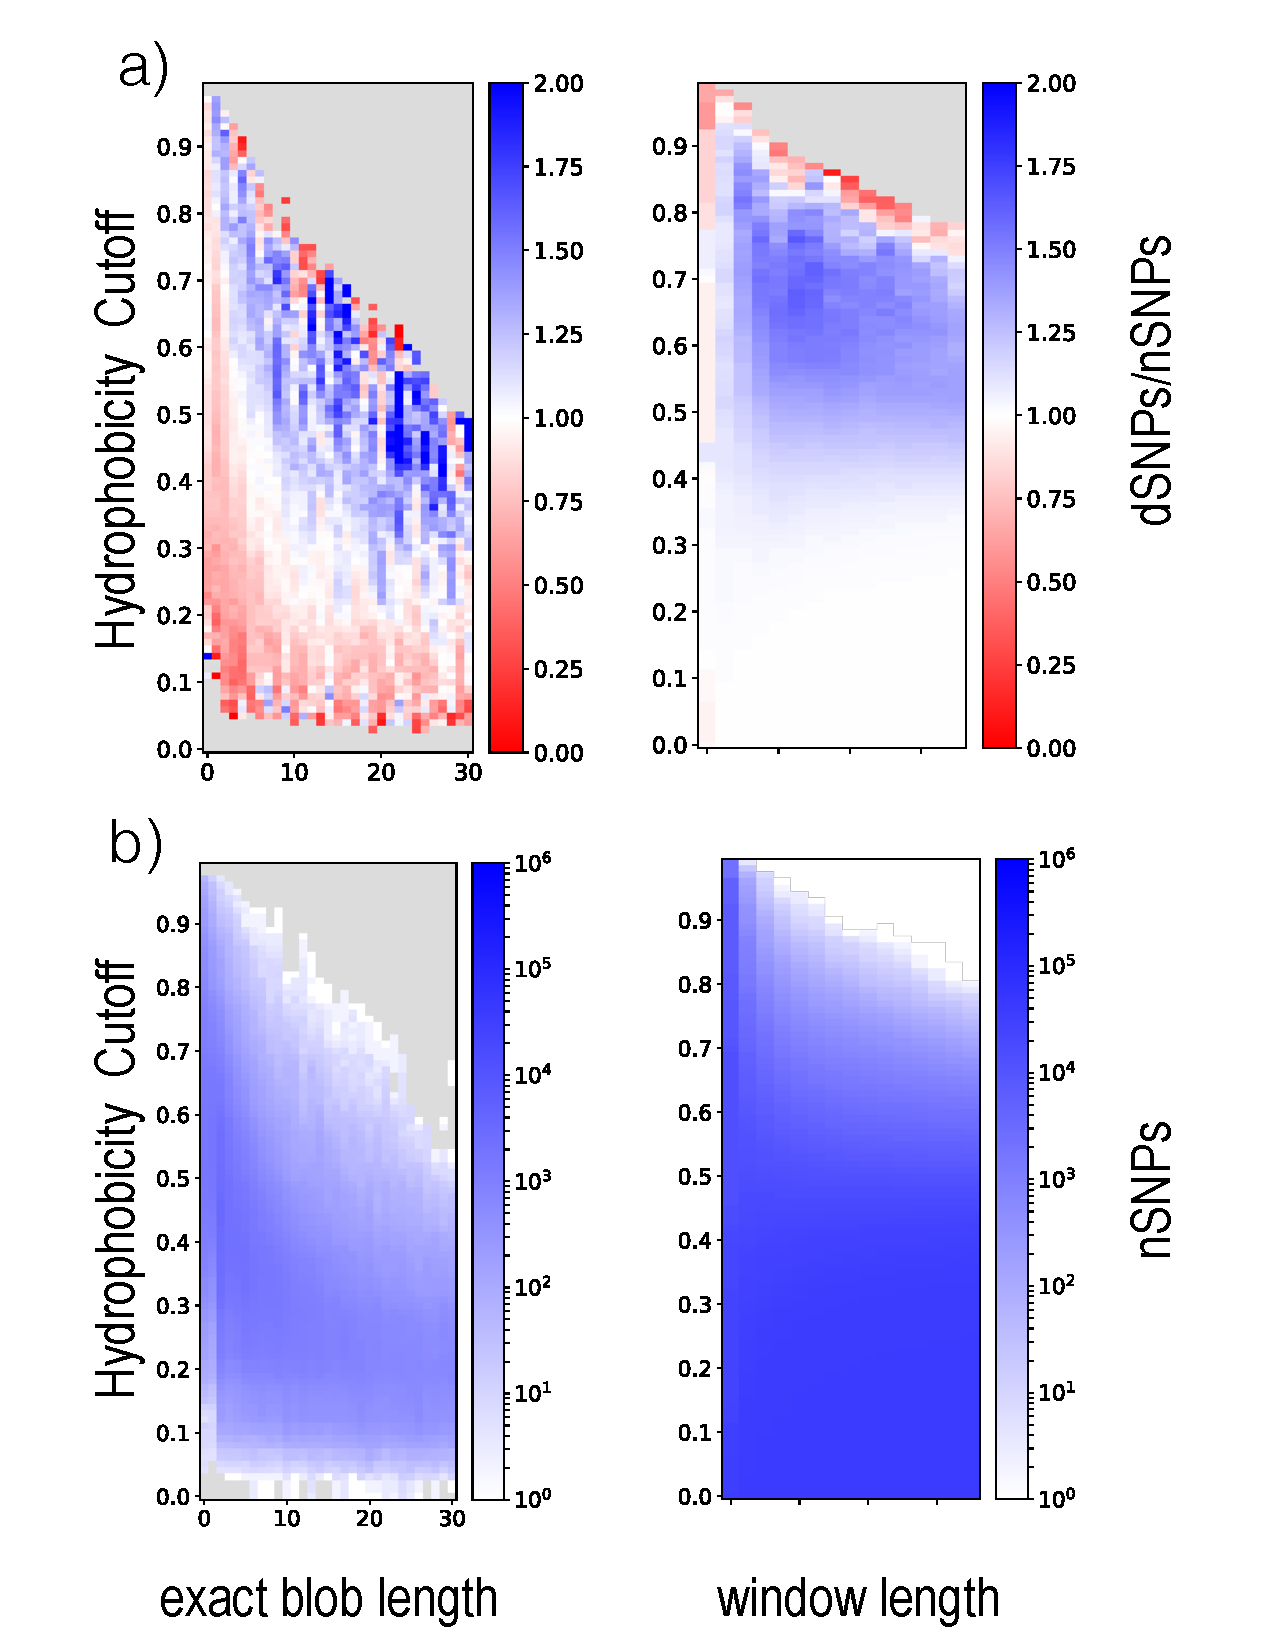
\includegraphics[width=0.6\textwidth]{./figures/fig3.pdf}
\caption{{\bf \DIFadd{Expected heterozygosity of SNPs in Europeans as a function of blob hydrophobicity}} \DIFadd{The black line shows the average expected heterozygosity $\het$ for (a) \nSNPs and (b) \dSNPs in h-blobs, determined using unconstrained threshold blobulation ($\Lmin=4$) and binned by the resulting maximum SNP hydrophobicity $\cmax$. $\cmax$ bins have width $\Delta \cmax=0.25$ and error bars represent standard errors in the mean for that bin. Only SNPs where at least one of two alleles are in an annotated h-blob are considered. Frequencies are taken from the gnomAD cohort of non-Finnish Europeans. The brown line is the average heterozygosity for all SNPs with $\cmax < 0.5$ (the line is solid for $\cmax$<0.5 and dashed for $\cmax$ > 0.5). The background null distributions generated from randomized permutations are shown as brown shaded regions, with the null percentiles as shown in the legend on the right. }}
\label{fig:het_v_hydromax} 
\end{SCfigure*}
}\fi
\DIFaddend 

\DIFdelbegin \DIFdel{For population frequency data we use gnomAD v3 SNP frequency data for $N \sim 32,000$ }\DIFdelend \DIFaddbegin \DIFadd{The results of stratifying the genetic diversity of SNPs by their surrounding maximum blob hydrophobicity is shown in Figure \ref{fig:het_v_hydromax} (see SI Dataset 3). 
%DIF > The results of stratifying the genetic diversity of SNPs by their surrounding blob hydrophobicity is shown in Figure \ref{fig:het_v_hydromax}, where the mean heterozygosity of nSNPs and dSNPs are binned by the maximal blob hydrophobicity ($\cmax$) for each SNP. 
%DIF > The maximal hydrophobicity, $\cmax$, is calculated for each SNP (based on the reference allele) by finding the largest $\Ht$ for which the residue resides in an h-blob with length as large as the given $\Lmin$ (see Materials and Methods). 
%DIF > In this analysis we use a minimum blob length of $\Lmin=4$, and blobulate in increments of $\Delta H^* = 0.05$ to identify $\cmax$ with a resolution of $0.05$. 
The population frequencies are based on }\DIFaddend non-Finnish Europeans \cite{Karczewski2021}\DIFdelbegin \DIFdel{. }\DIFdelend \DIFaddbegin \DIFadd{, for which the UniProt dSNP and nSNP functional annotations are expected to be reasonably accurate.
%DIF > For a given residue $i$ we find the largest hydrophobicity threshold $\Ht$ for which it resides in an h-blob of length at least $\Lmin$; this largest hydrophobicity threshold defines $\cmax$ for residue $i$. Here we use a minimum blob length of $\Lmin=4$, and blobulate in increments of $\Delta H^* = 0.05$ to identify $\cmax$ with a resolution of $0.05$. For population frequency data, we use the gnomAD v3 SNP frequencies for $N \sim 32,000$ non-Finnish Europeans \cite{Karczewski2021}. The average heterozygosity of nSNPs over this cohort is $\langle \het \rangle_{\rm nSNP} = 0.14$, while that of dSNPs is nearly 50 times lower, $\langle \het \rangle_{\rm dSNP} = 0.0029$. 
}\DIFaddend The average heterozygosity of \DIFdelbegin \DIFdel{non disease-associated SNPs over this cohort is $\langle \het \rangle_{\rm nSNP} = 0.14$}\DIFdelend \DIFaddbegin \DIFadd{nSNPs in low hydrophbicity domains ($\cmax\le 0.25$) is $0.125$ (Figure ~\ref{fig:het_v_hydromax}A)}\DIFaddend , while that \DIFdelbegin \DIFdel{of disease-associated SNPs is nearly 50 }\DIFdelend \DIFaddbegin \DIFadd{for dSNPs is 40 }\DIFaddend times lower, \DIFdelbegin \DIFdel{$\langle \het \rangle_{\rm dSNP} = 0.0029$. Figure \ref{fig:het_v_hydromax} shows the mean heterozygosity of nSNPs and dSNPs binned by the maximal blob hydrophobicity ($\cmax$)for each SNP (see Methods). The null background is generated by random permutation of the heterozygosity assigned to each SNP, corresponding to the null hypothesis that there is no correlation between SNP heterozygosity and blob properties. Both }\DIFdelend \DIFaddbegin \DIFadd{0.003 (Figure ~\ref{fig:het_v_hydromax}B). For both }\DIFaddend nSNPs and dSNPs\DIFdelbegin \DIFdel{show }\DIFdelend \DIFaddbegin \DIFadd{, the genetic diversity shows }\DIFaddend a significant departure \DIFaddbegin \DIFadd{from the neutral expectation }\DIFaddend (outside the $1^{\rm st}-99^{\rm th}$ null percentiles) \DIFdelbegin \DIFdel{in mean heterozygosity from null expectations }\DIFdelend for the largest $\cmax$ bin, $\cmax \geq 0.75$. %DIF < Compared to the heterozygosity at neutrally evolving regions of the genome, $H_0$, both purifying selection (the removal of almost all new functional alleles) and positive selection (the preference for a single functional allele) lowers $H$ below $H_0$ \cite{charlesworth_1993}. For regions of the genome expected to be under purifying selection, such as functional gene coding regions, the relaxation of purifying selection will lead to increased heterozygosity as $H$ returns to $H_0$, as have been document in human populations \cite{somel_2013,pierron_2013}. Balancing selection (maintenance of multiple functional alleles) increases $H$ above $H_0$. Population substructure and can also increase $H$, but such effects would be expected to have the same impact genome-wide, regardless of blobulation categories, and therefore would not cause $H$ to vary between categories or $\cmax$ bins as shown in Figure \ref{fig:het_v_hydromax}. 
For nSNPs, the heterozygosity is larger than expected \DIFdelbegin \DIFdel{in the highest $\cmax$ bin }\DIFdelend ($>99^{\rm th}$ null percentile), \DIFdelbegin \DIFdel{consistent with relaxed purifying selection or increased }\DIFdelend \DIFaddbegin \DIFadd{indicative of }\DIFaddend balancing selection. In contrast, for dSNPs the heterozygosity \DIFdelbegin \DIFdel{in the largest $\cmax$ bin }\DIFdelend is smaller than expected \DIFdelbegin \DIFdel{under the null }\DIFdelend ($<1^{\rm st}$ null percentile)\DIFdelbegin \DIFdel{. Given that disease risk alleles are almost always ``new'' deleterious mutations, we surmise that this decrease in $\het$ is due to }\DIFdelend \DIFaddbegin \DIFadd{, indicative of }\DIFaddend greater purifying selection \DIFdelbegin \DIFdel{acting to remove the risk allele}\DIFdelend \DIFaddbegin \DIFadd{in highly hydrophobic blobs}\DIFaddend . In other words, the disease-associated alleles in highly hydrophobic blobs appear to be more deleterious than disease-associated alleles in lower hydrophobicity blobs. 

The results here may explain the non-monotonic behavior of the dSNP-to-nSNP enrichment seen in Figure \ref{blob_vs_window}\DIFdelbegin \DIFdel{c and d }\DIFdelend \DIFaddbegin \DIFadd{C,D }\DIFaddend for both the \DIFdelbegin \DIFdel{blobulation and moving windows }\DIFdelend \DIFaddbegin \DIFadd{moving window and blobulation }\DIFaddend calculations. The thin band of ``red'' over the bins with the highest hydrophobic threshold that still contain data indicates a depletion in the number of dSNPs relative to nSNPs. Before examining the population frequency data, it was not clear if the lack of dSNPs relative to nSNPs is due to increased selection against dSNPs\DIFdelbegin \DIFdel{in those blobs}\DIFdelend , increased balancing selection for nSNPs\DIFdelbegin \DIFdel{in those blobs}\DIFdelend , or a mixture of both. In this section we have shown that the heterozygosity of dSNPs decreases with higher blob hydrophobicity while the heterozygosity of nSNPs rises with blob hydrophobicity. This suggests that the depletion observed in \DIFdelbegin \DIFdel{Figure \ref{blob_vs_window}c and d }\DIFdelend \DIFaddbegin \DIFadd{Figures \ref{blob_vs_window}C,D }\DIFaddend in the high hydrophobicity regions is caused by both increased selection against disease-associated alleles and increased selection for the maintenance of \DIFdelbegin \DIFdel{functional }\DIFdelend \DIFaddbegin \DIFadd{polymorphisms in the }\DIFaddend non disease-associated \DIFdelbegin \DIFdel{alleles}\DIFdelend \DIFaddbegin \DIFadd{variants}\DIFaddend . 

%DIF < why there is a decrease in dSNP enrichment at the highest hydrophobic thresholds for fixed blob length, as can be seen in Figure \ref{blob_vs_window}b, for both the blobulation and moving windows calculations. The thin band of ``red'' over the bins with the highest hydrophobic threshold that still contain data indicates a de-enrichment in the number of dSNPs relative to nSNPs. At the outset it is not clear if the lack of dSNPs relative to nSNPs is due to increased selection against dSNPs in those blobs or increased selection for nSNPs in those blobs, or a mixture of both. In this section we have shown that the heterozygosity of dSNPs decreases as $\cmax$ increases while that of nSNPs rises. This suggests that the de-enrichment is likely caused by both increased selection against disease-associated alleles and increased selection for the maintenance of functional non disease-associated alleles. Overall it underscores the main finding that highly hydrophobic blobs are enriched for SNPs under selection based on distortions in the population genetic diversity.
\DIFdelbegin %DIFDELCMD < 

%DIFDELCMD < %%%
\DIFdelend We tested whether the trends observed in Figure \ref{fig:het_v_hydromax} are specific to non-Finnish Europeans by performing the same analysis \DIFdelbegin \DIFdel{on the gnomAD East Asian frequency data set of approximately $\sim 1,500$ individuals . Although }\DIFdelend \DIFaddbegin \DIFadd{based on East Asian population frequencies (see SI Figure 1 and SI Dataset 4).
%DIF > on the gnomAD East Asian frequency data set of approximately $\sim 1,500$ individuals. 
The East Asian frequency dataset contains an order of magnitude fewer individuals than the non-Finnish European data, $n\sim 1,500$ }{\it \DIFadd{vs}} \DIFadd{$n\sim 32,000$ individuals, which means the frequency resolution is worse than for the non-Finnish European data. Consequently, }\DIFaddend we do not observe the same level of statistical significance, \DIFaddbegin \DIFadd{but }\DIFaddend we do find the same trends as in the European cohort: for nSNPs there is increasing heterozygosity with increasing $\cmax$ and for dSNPs the heterozygosity decreases with increasing $\cmax$\DIFdelbegin \DIFdel{(Figure S1)}\DIFdelend . The stratification of genetic diversity with blob properties appears to be a feature shared across diverse human populations.

\DIFdelbegin \DIFdel{In order to provide some context for }\DIFdelend \DIFaddbegin \DIFadd{For additional context on }\DIFaddend the proteins containing the blobs in the $\cmax\geq 0.75$ bin we use gene-ontology and pathway enrichment tests \DIFaddbegin \DIFadd{(see Materials and Methods)}\DIFaddend . The nSNPs found in blobs with $\cmax\geq 0.75$ are distributed across a subset of proteins ($n=635$), which we test against the background of all proteins containing nSNPs ($N=10,406$).  For the dSNPs, there are $n=179$ proteins containing the $\cmax\geq 0.75$ SNPs and a total background of \DIFdelbegin \DIFdel{$N=1803$ }\DIFdelend \DIFaddbegin \DIFadd{$N=1,803$ }\DIFaddend proteins containing a dSNP. Both the $\cmax \geq 0.75$ nSNP and dSNP proteins are most enriched for being located in or on a membrane (\DIFdelbegin \DIFdel{Data sets 2 and 3}\DIFdelend \DIFaddbegin \DIFadd{SI Dataset 4}\DIFaddend ), as expected for proteins containing highly hydrophobic blobs. In terms of molecular function and biological process, however, the nSNPs and dSNPs differ in their enriched ontologies. The $\cmax\geq 0.75$ nSNPs are enriched for olfactory processes, chemical sensing, and signal transduction. This accords with previous observations that olfactory-related genes exhibit signs of \DIFaddbegin \DIFadd{balancing selection\mbox{%DIFAUXCMD
\cite{Alonso2008} }\hspace{0pt}%DIFAUXCMD
and/or }\DIFaddend relaxed purifying selection\DIFdelbegin \DIFdel{relative to other genic regions }\DIFdelend \cite{Pierron2013}. This analysis has essentially re-identified this same feature of greater diversity in chemical sensing pathways, found here because the increased genetic diversity is specifically present in highly hydrophobic subdomains of those proteins. In contrast, the $\cmax\geq 0.75$ dSNPs are enriched for cation and small molecule trans-membrane transport proteins. These SNPs reside in proteins enriched for critical membrane bound transporters, consistent with the signal of higher functional constraint.
%DIF < %%%%%%%%%%%%
%DIF < If hydrophobic blobs have served a conserved functional role over evolutionary timescales then their DNA sequences are expected to show evidence of selection in order to maintain the relevant hydrophobic properties. Additionally, if hydrophobic blobs provide subdomains of high domain-domain and domain-membrane interactions, we may expect an enrichment of functional SNPs under selection. One consequence of selection over a genomic region is a distortion in the genetic diversity present in that region compared to neutrally evolving parts of the genome \cite{mcvicker_2009,lohmueller_2011}. Here we only consider genetic diversity as measured by the population heterozygosity, $H\equiv 2\nu(1-\nu)$, where $\nu$ is the frequency of the coded allele. Compared to the heterozygosity at neutrally evolving regions of the genome, $H_0$, both purifying selection (the removal of almost all new functional alleles) and positive selection (the preference for a single functional allele) lowers $H$ below $H_0$ \cite{charlesworth_1993}.  In contrast, balancing selection (maintenance of multiple functional alleles) increases $H$ above $H_0$ \cite{somel_2013,pierron_2013}. Population substructure can also increase $H$, but such effects would be expected to have the same impact genome-wide regardless of blobulation categories, and therefore would not cause $H$ to vary between categories. Any genome-wide difference in $H$ between different types or categorizations of genomic regions is a signal of differential selection between these types of regions. As selection only operates on regions of the genome that are functional or linked to functional variation, observing significant differential heterozygosity is a strong indicator that the categorization is stratifying functional regions.

%DIF < We test how well blobulation delineates functional elements by testing for differences in $H$ when SNPs are stratified by their surrounding blob properties. %Moreover, if highly hydrophobic blobs are enriched for biological function compared to less hydrophobic blobs, then we would expect to see differences in selection on genetic variants found in h-blobs as a function of blob hydrophobicity thresholds. 
%DIF < Under the hypothesis that hydrophobic blobs are functional subdomains we would expect to see the greatest deviations in mean heterozygosity from background levels in the high hydrophocity blobs.
%DIF < Purifying selection tends to remove all functional alleles that differ from the most fit sequence. Often the most fit allele is the most common and consequently often the reference allele. This functional alleles or newly functional alleles
%DIF < Regions under purifying selection have lowered genetic diversity, which is the evolutionary feature we examine here. Population heterozygosity, $H\equiv 2\nu(1-\nu)$ for biallelic variants with frequency $\nu$ for the coded allele, is a basic measure of genetic variation present in a population. If hydrophobic blobs have had no impact of fitness then we would expect that $H$ would not differ between blobs with different properties.
%DIF < For input frequency data we use the gnomAD SNP frequency data for non-Finnish Europeans. This whole-exome sequencing meta-cohort contains roughly $\sim 40,000$ individuals, providing allele frequency data as low as 1/80,000 $\sim 0.001 \%$. 29,653 nSNPs and 6,372 dSNPs overlap with this gnomAD frequency dataset. The average heterozygosity of non disease-associated SNPs over this cohort is $\langle H \rangle_{\rm nSNP} = 0.14$, while that of disease-associated SNPs is nearly 50 times lower, $\langle H \rangle_{\rm dSNP} = 0.0029$. This reflects the much higher degree of purifying selection on the disease-associated SNPs in general, as expected. 
\DIFaddbegin \subsection*{\DIFadd{\dSNP enrichment emerges in shorter and more weakly-hydrophobic blobs for aggregating proteins}}
\DIFaddend 

%DIF < %%%%%%%%%%%%%%%%%%%%
%DIF <  Hydrophobicity-max dependence
%DIF < %%%%%%%%%%%%%%%%%%%%
%DIF < In order to test for the impact of the surrounding blob's hydrophobicity on SNP heterozygosity, we first partition SNPs by the maximum blob hydrophobicity threshold for which at least one of the alleles remains in an h-blob, defined as $\cmax$. \matt{move this sentence methods}Each SNP can have it's own $\cmax$ value. We set a minimum h-blob length of $\Lmin=4$ amino acids. The blob length at $\cmax$, $\Lmax$, is not fixed and $\cmax$ does not always correspond to blobs of length $\Lmin$. We consider nSNPs and dSNPs separetly, so as to remove the already known factor of disease-association, which we know has a large impact on the heterozygosity from the above tabulation of the means. We focus on the subtler effects of functional stratification among nSNPs and, separately, among dSNPs. We bin SNPs into four $\cmax$ bins of width $\Delta \cmax = 0.25$ and compute the mean SNP heterozygosity within each bin. The null distribution for each bin is computed based on randomized permutation of the SNP heterozygosity among the input SNP set. \matt{What is the test?}
\DIFdelbegin %DIFDELCMD < 

%DIFDELCMD < %%%
%DIF < As shown in Figure \ref{fig:cmax_v_het}, both nSNPs and dSNPs show a significant departure in mean heterozygosity from null expectations for the largest $\cmax$ bin, $\cmax \geq 0.75$. In each of the three lower $\cmax$ bins the mean heterozygosity is not significantly different than what is expected from the null (within $10-90^{\rm th}$ percentiles of the null distribution). For nSNPs, the heterozygosity is larger than expected in the highest $\cmax$ bin ($>99^{\rm th}$ null percentile), consistent with increased balancing selection. In contrast, for dSNPs the heterozygosity in the largest $\cmax$ bin is smaller than expected under the null ($<1^{\rm st}$ null percentile), consistent with increased purifying selection.   
%DIF < In order to provide some context for the proteins containing the blobs in the $\cmax\geq 0.75$ bin we use gene-ontology enrichment. The nSNPs in $\cmax\geq 0.75$ blobs are contained in $n=635$ proteins, which we test against the background of all proteins containing nSNPs ($N=10,406$).  For the dSNPs, there are $n=179$ proteins containing the $\cmax\geq 0.75$ SNPs and a total background of $N=1803$ proteins containing a dSNP. Both the $\cmax \geq 0.75$ nSNP and dSNP proteins are most enriched for being located in or on a membrane (see SI Tables ``GO nSNP'' and ``GO dSNP''), as expected for proteins containing highly hydrophobic blobs. In terms of molecular function and biological process, however, the nSNPs and dSNPs differ in their enriched ontologies. The $\cmax\geq 0.75$ nSNPs are enriched for olfactory processes, chemical sensing, and signal transduction. This accords with previous observations that olfactory-related genes tend to be more genetically diverse compared to most other parts of the genome, due to the presumed evolutionary fitness of being able to smell or taste a greater variety of chemical compounds \cite{pierron_2013}. This analysis has essentially re-identified this same feature of greater balancing selection in chemical sensing pathways, found here because the increased genetic diversity is specifically present in highly hydrophobic subdomains of those proteins. The $\cmax\geq 0.75$ dSNPs are enriched for (cat-)ion and small molecule transmembrane transport proteins. These SNPs reside in proteins enriched for critical membrane bound transporters, consistent with the signal of higher functional constraint.
%DIFDELCMD < 

%DIFDELCMD < %%%
%DIF < Among nSNPs and among dSNPs we find that the mean SNP heterozygosity is not constant with respect to the surrounding blob hydrophobicity. As one method to quantify this, for each SNP we recorded the maximum hydrophobicity threshold for which that SNP remained in an h-blob. We denote this maximum hydrophobicity $\cmax$. For neutral SNPs, the heterozygosity is relatively contanst at $\sim 0.14$ up to $\cmax\sim 0.7$, with higher heterozygosity for SNPs with $\cmax > 0.7$ (Figure \ref{fig:cmax_v_het}a). This points towards either greater balancing selection or greater European population substructure for nSNPs in blobs with $\cmax\geq 0.7$. We test for statistical significance by permutation tests that randomize the heterozygosity assigned to each nSNP. Based on the permutation tests on $\cmax$ bins of width $0.1$, we find two bins with mean heterozygosities more extreme than 95\% of the randomized background. The $\cmax$ bin $[0.3,0.4)$ has lower mean $H$ than 95\% randomized values over this bin, despite the small deviation in raw value. In contrast, the $\cmax$ bin $[0.7,0.8)$ has a higher mean heterozygosity than 95\% of randomized values for this bin.  
%DIFDELCMD < 

%DIFDELCMD < %%%
%DIF < In order to gain further insight into the proteins containing blobs in the two $\cmax$ bins with significant heterozygosity deviations, we used gene ontology enrichment on the subset of proteins containing these blobs against the background of all proteins containing an nSNP. As shown in Table XXX, these proteins are significantly enriched for being located in the plasma membrane, as expected. These proteins are also enriched for olfactory and sensory perception molecular functions \ref{fig:cmax_v_het}. It is well known that olfactory-related genes tend to be more genetically diverse compared to most other parts of the genome, due to the presumed evolutionary fitness of being able to smell or taste a greater variety of chemical compounds \cite{pierron_2013}. In the case of nSNPs, blobulation and stratification by the maximum blob hydrophobicity has re-identified this same feature of greater genetic diversity in specific subdomains in olfactory-related chemical sensing and signal transduction pathway proteins.
%DIFDELCMD < 

%DIFDELCMD < %%%
%DIF < For disease-associated SNPs we also find a significant deviation in genetic heterozygosity for the most hydrophobic blobs, though the direction of effect is in the opposite direction from nSNPs: dSNP heterozygosity is significantly decreased for the most hydrophobic blobs, $\cmax\geq 0.7$ (Figure \ref{fig:cmax_v_het}b). This indicates that dSNPs in highly hydrophobic blobs are under the most selective constraint. As shown in Table 2, gene ontology enrichment of proteins containing the SNPs in the $\cmax\geq 0.7$ blobs shows enrichment for membrane bound cellular location, as expected for proteins containing highly hydrophobic segments and just as we find for nSNPs with $\cmax\geq 0.7$. However, for dSNPs the enriched molecular functions all relate to ion and small molecular transporters involved in metabolism and homeostasis. Membrane transporter activity refers to the active transport of ions and small molecules across a membrane against the diffusion gradient, and is thus critical machinery in many cellular systems. Thus blobulation and stratification by the maximum blob hydrophobicity demonstrates that among disease-associated SNPs there is discernible increased purifying selection in highly hydrophobic blobs. These blobs reside in proteins enriched for critical membrane bound transporters, consistent with the signal of higher functional constraint that we observe. 
%DIFDELCMD < 

%DIFDELCMD < %%%
%DIF < As a function of increasing blob hydrophobicity (Figure \ref{fig:blob_het}a,c), we find that the genetic variation increases for neutral SNPs and decreases for disease-associated SNPs. 
%DIF < For both types of SNPs $H$ remains relatively constant for hydrophobicities $\leq 0.4$.  In contrast, for disease-associated SNPs the heterozygosity decreases by a factor of $\sim 8$ over a similar hydrophobicity range, with a particularly sharp drop in heterozygosity for blob hydrophobicities $\geq 0.7$.
%DIFDELCMD < 

%DIFDELCMD < %%%
%DIF < %%%%%%%%%%%%%%%%%%%%
%DIF <  Joint dependence
%DIF < %%%%%%%%%%%%%%%%%%%%
%DIF < The results here also indicate why there is a decrease in dSNP enrichment at the highest hydrophobic thresholds for fixed blob length, as can be seen in Figure \ref{blob_vs_window}b, for both the blobulation and moving windows calculations. The thin band of ``red'' over the bins with the highest hydrophobic threshold that still contain data indicates a de-enrichment in the number of dSNPs relative to nSNPs. At the outset it is not clear if the lack of dSNPs relative to nSNPs is due to increased selection against dSNPs in those blobs or increased selection for nSNPs in those blobs, or a mixture of both. In this section we have shown that the heterozygosity of dSNPs decreases as $\cmax$ increases while that of nSNPs rises. This suggests that the de-enrichment is likely caused by both increased selection against disease-associated alleles and increased selection for the maintenance of functional non disease-associated alleles. Overall it underscores the main finding that highly hydrophobic blobs are enriched for SNPs under selection based on distortions in the population genetic diversity.
%DIFDELCMD < 

%DIFDELCMD < %%%
%DIF < The joint dependence of SNP heterozygosity on blob hydrophobicity and blob length is more complex. This is partly due to the highly correlated structure of the data, as the blob size a SNP resides in depends upon the hydrophobicity threshold considered. All else being equal, as the hydrophobicity threshold increases the blobs become shorter. %In general, if a SNP is a blob of size $\ell_0$ at threshold $c_0$, then it is in a blob with a smaller size at a higher hydrophobicity threshold, $\ell_1 < \ell_0$ for $c_1 > C_0$, i.e. we expect an negative correlation between blob size and the hydrophobicity threshold.
%DIF < Figures \ref{fig:blob_het}b,e shows the heterozygisity for nSNPs and dSNPs over the two blob properties of size and hydrophobicity, $(L,c)$. For both SNP types there is an overall negative correlation between blob size $L$ and hydrophobicity $c$, as expected. 
%DIFDELCMD < 

%DIFDELCMD < %%%
%DIF < For non-disease associated SNPs in blobs with hydrophobicity $c>0.4$, we observe a deficit of heterozygosity in the shortest blobs and an excess of heterozygosity in the longer blobs. 
%DIFDELCMD < 

%DIFDELCMD < %%%
%DIF < We observe that the nSNP heterozygosity shows a relative increase in a roughly diagonal patch of blob property space, from $L=40$ and $c=0.4$ to $L=0$ and $c=0.9$. GO enrichment of the genes in this patch (boxes B,C in \ref{fig:blob_het}) show enrichment for G-coupled receptor signalling and olfactory-related function.  
%DIFDELCMD < 

%DIFDELCMD < %%%
%DIF < For dSNPs in blobs with hydrophobicities between $0.3\leq c \leq 0.5$ there is a noticeable drop in heterozygosity for blobs between $30-60$ in length (box "B" in \ref{fig:blob_het}). Gene ontology enrichment of the genes containing those blobs shows that these are highly enriched for membrane transport and transporter activity. We used GO enrichment to interrogate three additional regions of blob properties that show a relative increase in heterozygosity compared to other dSNPs, shown as boxes A,C, and D in \ref{fig:blob_het}. Region A is enriched for several GO terms consistent with membrane ion transporters. 
%DIFDELCMD < 

%DIFDELCMD < %%%
%DIF < The observed heterozygosity fluctuations do not appear to be due to statistical noise from the finite sampling nor a specific artifact of non-Finnish Europeans. To assess the degree of sampling noise we randomized the frequency assigned to each SNP for $R=500$ replicates, with the randomization done separately among nSNPs and dSNPs. This provides the background distribution under the hypothesis that there is no correlation between blob properties and heterozygosity. As shown in Figure \ref{fig:blob_het}c the observed mean value is greater than 2-$\sigma$ above the global mean for a portion of the blob property space. Figure \ref{fig:blob_het}d. To assess whether the trends observed in Figure \ref{fig:blob_het} are specific to non-Finnish Europeans or not, we performed the same analysis on the gnomAD East Asian frequency dataset of approximately $\sim 3000$ individuals. We find the same trends as in the European cohort (SI Figure XXX), demonstrating the stratification of genetic diversity with blob properties appears to be a feature shared across diverse human populations.
%DIFDELCMD < 

%DIFDELCMD < %%%
%DIF < When the heterozygosity is stratified by the blob hydrophobocity minimum  we find two different patterns for non-disease-associated and disease-associated SNPs. For non-disease-associated SNPs there is a significant positive correlation between heterozygosity and blob hydrophobicity. For disease-associated SNPs we observe the reverse: there is a small but significant negative correlationb between heterozygosity and blob hydrophobicity.
%DIFDELCMD < 

%DIFDELCMD < %%%
%DIF < \subsection*{Comparing \dSNPs and \nSNPs blob types in aggregating proteins}
\subsection{\DIFdel{\dSNP enrichment emerges in shorter and more weakly-hydrophobic blobs for aggregating proteins}}
%DIFAUXCMD
\addtocounter{subsection}{-1}%DIFAUXCMD
%DIFDELCMD < 

%DIFDELCMD < \begin{figure}[!ht]
%DIFDELCMD < \includegraphics[width=\textwidth,trim={0 0cm 0 0cm},clip]{./figures/figS2.pdf}
%DIFDELCMD < %%%
%DIFDELCMD < \caption{%
{%DIFAUXCMD
%DIFDELCMD < {\bf %%%
\DIFdelFL{Blob hydrophobicity for SNPs in aggregating proteins.}%DIFDELCMD < } %%%
\DIFdelFL{a) Fraction of \nSNPs or \dSNPs that are found in either blob type (a) or \chargechar (b) in non-aggregating proteins and known-aggregating proteins. c) is the fraction of \chargechar in each blob type in all proteins. The distribution in a, b and c are plotted with a cutoff and minimum blob length of 0.4 and 4 respectively. The effect of these parameters on proportion of SNPs in blob type is further discussed in Fig 2b. Error bars represent one standard error for multinomial distributed data. d) is same as Fig 2b but for non aggregating proteins and aggregating proteins. Enrichment of dSNPs in h-blob at fixed cutoff of 0.4 (e) or fixed blob length of 6.
%DIF < If enrichment or depletion in \dSNPs is significant  it is annotated with a star. 
 }}
%DIFAUXCMD
%DIFDELCMD < \label{agg_enrich} 
%DIFDELCMD < \end{figure}
%DIFDELCMD < 

%DIFDELCMD < %%%
\DIFdelend Side-chain hydrophobicity plays a well-established role in diseases involving aggregating proteins. \citep{ConchilloSole2007, Fang2013, Tartaglia2008}. In order to test whether the trends observed in \DIFdelbegin \DIFdel{Fig 2b }\DIFdelend \DIFaddbegin \DIFadd{Figure \ref{blob_vs_window}D }\DIFaddend are amplified in aggregating proteins, we separated aggregating proteins from the primary data set. Proteins involved in the formation of extracellular amyloid deposits or intracellular inclusions with amyloid-like characteristics are included in the \DIFdelbegin \DIFdel{"Aggregating proteins" }\DIFdelend \DIFaddbegin \DIFadd{``Aggregating proteins'' }\DIFaddend (28 proteins, 124 nSNPs, 330 dSNPs) subset, while all remaining proteins are labelled as \DIFdelbegin \DIFdel{"}\DIFdelend \DIFaddbegin \DIFadd{``}\DIFaddend Non-aggregating proteins\DIFdelbegin \DIFdel{"}\DIFdelend \DIFaddbegin \DIFadd{''}\DIFaddend . 

\DIFdelbegin \DIFdel{Figure ~\ref{agg_enrich}a shows the blob-type distribution of \nSNPs and \dSNPs, for both aggregating and non-aggregating proteins, using a mild hydrophobicity cutoff of 0.4. For \dSNPs, the blob distributions are insensitive to aggregating-tendencies of the protein: a given \dSNP in an aggregating protein is as likely to be found in an h-blob as if it were in a non-aggregating protein. We do still detect a small difference in enrichment because \nSNPs in aggregating proteins are found slightly less frequently in h-blobs }%DIFDELCMD < {\it %%%
\DIFdel{vs}%DIFDELCMD < } %%%
\DIFdel{\nSNPs in non-aggregating proteins.   
}%DIFDELCMD < 

%DIFDELCMD < %%%
\DIFdel{Stratifying the enrichment by hydrophobicity cutoff and blob length (as in Fig 2b of the main text) reveals a more informative quantitative shift. Figure ~\ref{agg_enrich}d compares the data from Fig 2b) with the same analysis for aggregating proteins. The highly-enriched (blue) band is shifted toward the origin for aggregating proteins, indicating that sensitivity to mutation is found in shorter and more weakly hydrophobic blobs. %DIF < Furthermore, few hydrophobic blobs with lengths greater than 30 were detected in this set of aggregating proteins. 
This shift is also visible in transects of the data along one row and one column, shown in Figure~\ref{agg_enrich}e and f. %DIF < These data reveal that the enrichment peak for aggregating proteins is both higher and shifted toward weaker hydrophobicity criteria, compared to non-aggregating proteins. 
These results are consistent with previous observations that the in vitro aggregation rate of unstructured polypeptide chains is proportional to hydrophobicity and inversely proportional to net charge\mbox{%DIFAUXCMD
\citep{DuBay2004}}\hspace{0pt}%DIFAUXCMD
.   %DIF <  used in Figs(\ref{c3_h_p_enrich} and \ref{blob_transition}), \dSNPs in aggregating proteins have a 1.33 fold enrichment in h blobs. In comparison, \dSNPs in non-aggregating proteins show a 1.15 fold enrichment in h blobs. This is consistent with the well-established hydrophobicity of aggregating proteins, including the hydrophobicity of amyloidogenic sequences~\citep{Tzotzos2010,Abskharon2019}, and further supports the hydrophobic regions of those proteins as particularly sensitive to mutation. Previously, de Groot et al.~\citep{Groot2005} used an in vivo method to study the aggregation propensity of each amino acids and found that high hydrophobic residues have high aggregation tendencies. 
}%DIFDELCMD < 

%DIFDELCMD < %%%
%DIF < More significantly, the enrichment for \dSNPs in the h blobs of aggregating proteins increases steadily as the requirements for h blobs are made stricter, reaching a maximum of 3.26 enrichment for blobs meeting a 0.53 hydrophobicity cutoff (Fig~\ref{agg_enrich}b).   In contrast, non-aggregating proteins are relatively insensitive to hydrophobic cutoff, reaching a maximum enrichment of less than 1.5 fold.  
%DIFDELCMD < 

%DIFDELCMD < %%%
%DIF < In order to test blobulation as a meaningful approach for analyzing sequences, we tested whether any blob type is correlated with a higher incidence of disease-causing mutations. For each SNP, we applied the blobulation approach on the entire protein sequence (Fig~\ref{c3_h_p_enrich}a) as described in Methods, and then further analyzed the blob containing the SNP. Specifically, we measured the enrichment of disease-associated SNPs (dSNPs) relative to non-disease-associated SNPs (nSNPs) for blobs characterized by \hydrochar{} and \chargechar{} (SNP dataset obtained from Uniprot; see Methods).  Fig~\ref{c3_h_p_enrich}c compares the distribution of blob \hydrochar~among \dSNPs and \nSNPs. We find that \dSNPs are enriched in h blobs by about 1.15 fold:  the fraction of \dSNPs in h blobs is 52\% while the fraction of \nSNPs in h blobs is about 45\%. This is consistent with our previous results from simulations of the long disordered BDNF prodomain, in which h blobs interacted frequently with each other, while p blobs did not form any specific interactions with the rest of the sequence.
%DIFDELCMD < 

%DIFDELCMD < %%%
\DIFdel{To test the significance of charge}\DIFdelend \DIFaddbegin \DIFadd{First, we used whole-sequence blobulation ($\Ht=0.4, \Lmin=4$) to compare the distributions for aggregating and non-aggregating proteins across two different approaches for blob characterization. In addition to the \hydrochar{} of previously discussed analyses}\DIFaddend , blobs were also assigned \chargechar{} (Figure~\ref{agg_enrich}\DIFdelbegin \DIFdel{b}\DIFdelend \DIFaddbegin \DIFadd{B}\DIFaddend ), which is the predicted globular phase according to Das and Pappu\citep{Das2013}\DIFdelbegin \DIFdel{and }\DIFdelend \DIFaddbegin \DIFadd{. This property is }\DIFaddend calculated using the fraction of positive and negative charges \DIFdelbegin \DIFdel{.
%DIF < blob-class (1,2,3,4,5) based on its fraction of charges (Das-Pappu classification). The Das and Pappu phase metrics predicts sequence compactness and is based on fraction of positively (f+) and negatively (f-) charged residues . 
Possible values of the blob \chargechar{} are }\DIFdelend \DIFaddbegin \DIFadd{in a blob, and is particularly relevant for IDPs. %DIF > Possible values of the blob \chargechar{} are 1 (Weak polyampholyte), 2 (Janus or boundary region), 3 (Strong polyampholyte), 4 (Negatively-charged strong polyelectrolyte), and 5 (Positively-charged strong polyelectrolyte). 
Nearly all structured proteins fall in the class }\DIFaddend 1 (Weak polyampholyte) \DIFdelbegin \DIFdel{, }\DIFdelend \DIFaddbegin \DIFadd{part of the Das-Pappu phase diagram. In contrast to structured proteins, IDPs can be found in all five Das-Pappu phases, including class }\DIFaddend 2 (Janus or boundary region), 3 (Strong polyampholyte), 4 (Negatively-charged strong polyelectrolyte), and 5 (Positively-charged strong polyelectrolyte). 
\DIFdelbegin \DIFdel{Sequences in class 1 have a low fraction of positively charged residues, and nearly all structured proteins fall in class 1. In contrast to structured proteins, IDPs can be found in all five Das-Pappu phases, particularly classes 3, 4, and 5. %DIF < Therefore the Das-Pappu \chargechar{} characterization provides a natural metric for distinguishing among sub-categories of IDPs with different functional behavior. 
}\DIFdelend \DIFaddbegin 

\DIFaddend The blob \hydrochar{} and \chargechar{} are fundamentally correlated; while blob \chargechar{} does not explicitly consider hydrophobicity, increasing the number of charged residues will reduce the average hydrophobicity of a blob. The extent of this correlation is shown in  Figure~\ref{agg_enrich}\DIFdelbegin \DIFdel{C}\DIFdelend \DIFaddbegin \DIFadd{A}\DIFaddend , which breaks down the fraction of \DIFdelbegin \DIFdel{h and p blobs }\DIFdelend \DIFaddbegin \DIFadd{h- and p-blobs }\DIFaddend that fall in each Das-Pappu \chargechar. As expected, most h blobs (90\%) fall in class 1 (weak polyampholyte), followed by 9\% in class 2 (Janus).  The \DIFdelbegin \DIFdel{p blobs }\DIFdelend \DIFaddbegin \DIFadd{p-blobs }\DIFaddend are more evenly distributed across classes, with the highest fraction (42\%) classified as strong polyelectrolytes.  %DIF < would be equivalent or better than blob \hydrochar{} for stratifying \grace{word choice?} disease-causing and non disease-causing SNPs. %
\DIFdelbegin %DIFDELCMD < 

%DIFDELCMD < %%%
%DIF < The distribution of \dSNPs and \nSNPs across blob \chargechar{} are shown in Fig~\ref{c3_h_p_enrich}d. 
%DIFDELCMD < 

%DIFDELCMD <  %%%
%DIF < In non-aggregating proteins \dSNPs are slightly enriched (1.09 fold) for weak polyampholyte class 1 blobs. 
\DIFdelend \DIFaddbegin \DIFadd{Figure ~\ref{agg_enrich}B and ~\ref{agg_enrich}C show the SNP distributions for blobs with different \hydrochar{} and \chargechar, respectively. }\DIFaddend Since there are five charge classes and only three hydrophobicity classes, we hypothesized that \DIFaddbegin \DIFadd{in non-aggregating proteins, }\DIFaddend blob \chargechar{} would \DIFdelbegin \DIFdel{be more precise }\DIFdelend \DIFaddbegin \DIFadd{have a stronger association with disease }\DIFaddend than blob \hydrochar{}\DIFdelbegin \DIFdel{for identification of functional protein segments. %DIF < More than half of both \dSNPs and \nSNPs are found in blobs that are only weakly charged, however, and 
}\DIFdelend \DIFaddbegin \DIFadd{. }\DIFaddend Instead, we found that the \DIFdelbegin \DIFdel{maximum \chargechar{} enrichment }\DIFdelend \DIFaddbegin \DIFadd{strongest dSNP enrichment as a function of \chargechar{} }\DIFaddend (1.09 fold \DIFaddbegin \DIFadd{, p $< 10^{-58}$ }\DIFaddend for weak polyampholyte blobs) is comparable or even slightly less than the enrichment found for \hydrochar{} (1.15 fold\DIFdelbegin \DIFdel{). This result suggests that even short contiguous stretches of weak hydrophobicity are as effective as charge distribution for predicting functional impact.   %DIF < Strong polyampholytes are depleted among \dSNPs (0.87 fold), which may indicate a relative decrease in blob-blob interactions, since strong polyampholytes tend to be highly solvent exposed. 
In the context of aggregating proteins, classification by charge yielded similar patterns as classification by hydrophobicity: \dSNPs have equivalent distributions regardless of protein aggregationtendency, while }\DIFdelend \DIFaddbegin \DIFadd{, P $< 10^{-122}$ for h-blobs). %DIF > This result suggests that even short contiguous stretches of weak hydrophobicity are as effective as charge distribution for predicting functional impact. 
}

\DIFadd{Furthermore, the charge-based and hydrophobicity-based classification schemes yield similar trends with protein aggregation:  Figure \ref{agg_enrich}B shows that a given \dSNP in an aggregating protein is just as likely to be found in an h-blob as if it were in a non-aggregating protein, and Figure \ref{agg_enrich}C shows an analogous result for \dSNPs in various charge classes. However, }\DIFaddend \nSNPs in aggregating proteins are \DIFdelbegin \DIFdel{significantly less likely to be found in }\DIFdelend \DIFaddbegin \DIFadd{found slightly less frequently in h-blobs or }\DIFaddend globular, weak-polyampholyte blobs (Class 1) than \DIFdelbegin \DIFdel{those }\DIFdelend \DIFaddbegin \DIFadd{\nSNPs }\DIFaddend in non-aggregating proteins. \DIFaddbegin \DIFadd{As a result, we do observe a small increase in overall dSNP enrichment for h-blobs/weak-polyampholyte blobs of aggregating proteins relative to non-aggregating proteins.
}\DIFaddend 

\DIFdelbegin \subsection*{\DIFdel{Disease-associated SNPs are enriched for mutations that change local blob characteristics and overall protein blob topology}}
%DIFAUXCMD
%DIFDELCMD < \ifnum%%%
\value{\DIFdel{includefigs}}%DIFAUXCMD
\DIFdel{>0 }%DIFDELCMD < {
%DIFDELCMD < \begin{figure}[!ht]
%DIFDELCMD < \center
%DIFDELCMD < 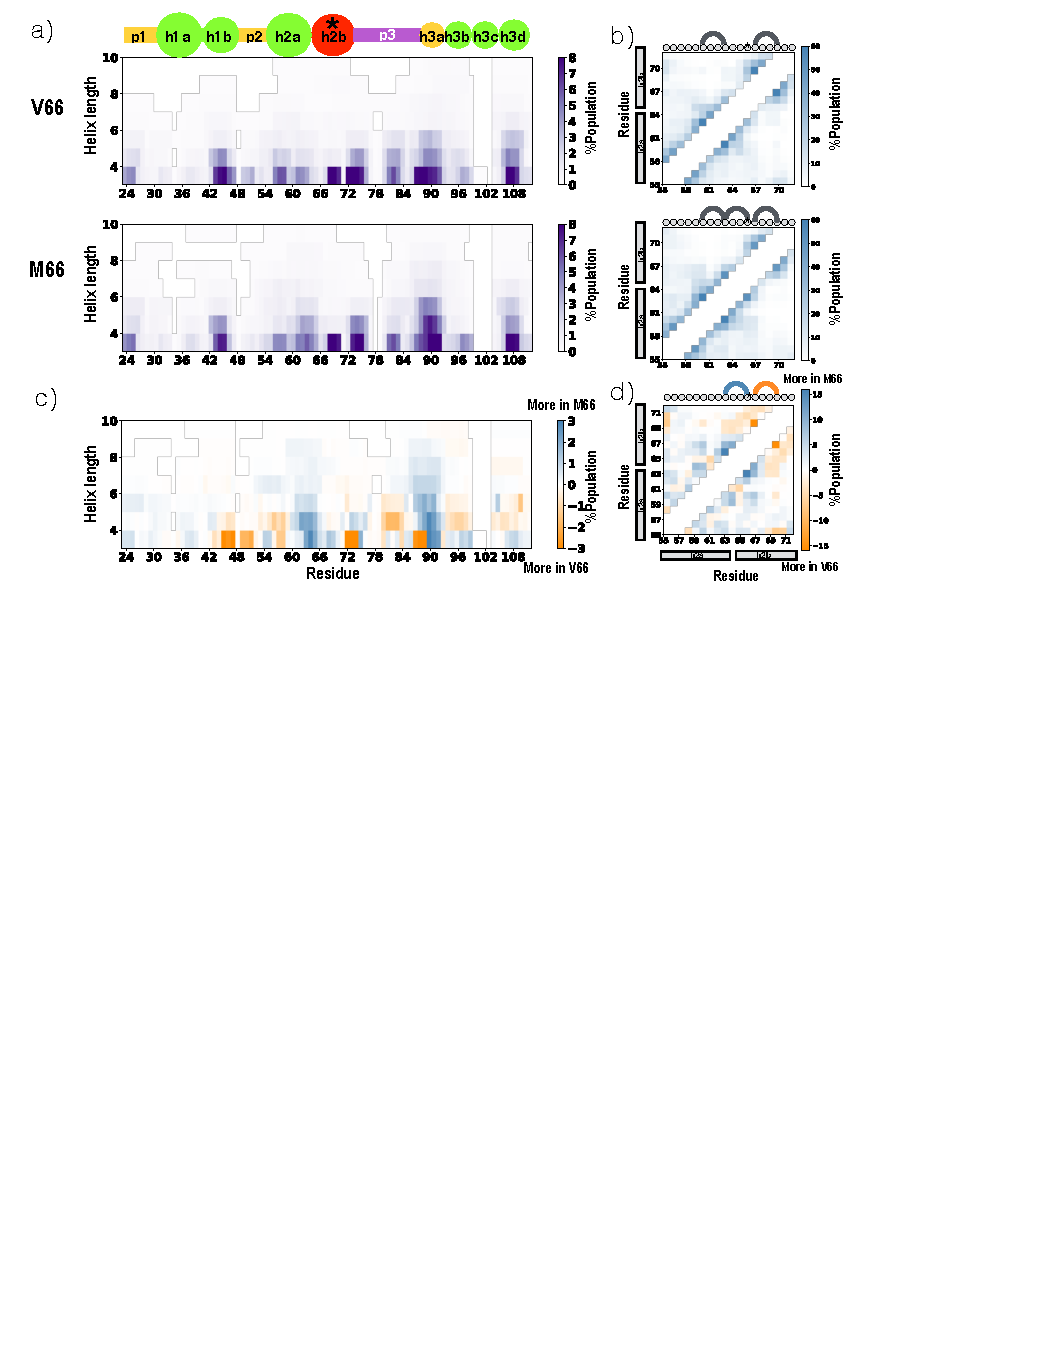
\includegraphics[width=0.5\textwidth,trim={0 0cm 0 0cm}]{./figures/fig5.pdf}
%DIFDELCMD < %%%
%DIF < \caption{{\bf Distribution of SNPs that change blob properties}  a) Fraction of \nSNPs or \dSNPs that change the blobular topology by either forming or dissolving an h-blob or by splitting one h-blob or merging two h-blobs. b) Fractions of \nSNPs or \dSNPs that induce a change in \hydrochar{} or \chargechar.  c) Fractions (as in a) broken down further by blob \hydrochar{} (left) or \chargechar{} (right) before (x axis) and after (y axis) the mutation.  Grid boxes are colored according to the overall fraction of corresponding \nSNPs (bottom) and the corresponding enrichment ratios (\dSNPs/\nSNPs) (top). Fewer than 1.5\% of SNPs involve class 4 and 5, and these data are not shown for readability. Significant enrichment or depletion in \dSNPs is annotated with one star (p $< 10^{-3}$) or two star (p $< 10^{-10}$).Errors bars in (a), (b) and (c) represent one standard error for multinomial distributed data. All plots used a mild hydrophobicity threshold of $\cmin=0.4$ and a minimum h- or p- blob length of $\Lmin=4$ residues.}
%DIFDELCMD < \caption{%
{%DIFAUXCMD
%DIFDELCMD < {\bf %%%
\DIFdelFL{Distribution of SNPs that change blob properties}%DIFDELCMD < }  %%%
\DIFdelFL{a) Fraction of \nSNPs or \dSNPs that change the blobular topology by either forming or dissolving an h-blob or by splitting one h-blob or merging two h-blobs. b) Fractions of \nSNPs or \dSNPs that induce a change in \hydrochar{} or \chargechar.  c) The enrichment of \dSNPs relative to \nSNPs that induce a specific blobular topology transition between the reference allele (x-axis) and the alternative allele (y-axis). This is shown for two blob properties, \hydrochar{} (left) and \chargechar{} (right). d) The overall proportion of \nSNPs that induce each of the blobular topology transitions shown in c).  Fewer than 1.5\% of SNPs involve charge classes 4 or 5, and these data are not shown for readability. Significant enrichment or depletion in \dSNPs is annotated with one star (p $< 10^{-3}$) or two stars (p $< 10^{-10}$). Errors bars in (a) and (b) represent one standard error for multinomial (a) or binomial (b) distributed data. In all cases blobulation is calculated using $\cmin=0.4$ and $\Lmin=4$.}}
%DIFAUXCMD
%DIF < d) show the average change in h-blob lengths between the reference and alternative allele, binned by the h-blob length. For each blob length bin, we compute the averages using the h-blob length for the reference and alternative alleles separately, and then take the mean of those two values. 
%DIF <  . Each bin has a minimum of 10 SNPs. The average change in direction in the h-blob length, with ``+1'' corresponding to the alternative allele having a longer h-blob than the reference allele, and conversely for ``-1''. The average magnitude of change in h-blob length.}
%DIFDELCMD < \label{c3_h_p_enrich} 
%DIFDELCMD < \end{figure}
%DIFDELCMD < }\fi
%DIFDELCMD < %%%
\DIFdelend %DIF > For dSNPs, the \hydrochar{} distributions are insensitive to aggregating-tendencies of the protein: a given \dSNP in an aggregating protein is just as likely to be found in an h-blob as if it were in a non-aggregating protein. 
%DIF > \dSNPs are equivalently distributed across hydrophobicity classes, regar, while Figure \ref{agg_enrich} C yields a similar result for charge classes.  regardless of protein aggregation tendency, while \nSNPs in aggregating proteins are significantly less likely to be found in globular, weak-polyampholyte blobs (Class 1) than those in non-aggregating proteins.  %The consistency of these results are consistent with previous evidence that the in vitro aggregation rate of unstructured polypeptide chains is proportional to hydrophobicity and inversely proportional to net charge\citep{DuBay2004}.  

\DIFdelbegin \DIFdel{The }\DIFdelend \DIFaddbegin \DIFadd{We then used the results from unconstrained-length blobulation to further stratify the \dSNP enrichment in aggregating proteins by hydrophobicity threshold $\Ht$ and blob length. The enrichment calculations from Figure \ref{blob_vs_window}d were partitioned between aggregating and non-aggregating proteins, and are shown in Figure ~\ref{agg_enrich}D. The highly-enriched (blue) band is shifted toward the origin for aggregating proteins, indicating that sensitivity to mutation is found in shorter and more weakly hydrophobic blobs. These results suggest that the differential distributions from whole-sequence blobulation in Figure~ \ref{agg_enrich}B and C reflect a difference in effective thresholds for non-aggregating proteins. 
}

\begin{SCfigure*}[\sidecaptionrelwidth][t]
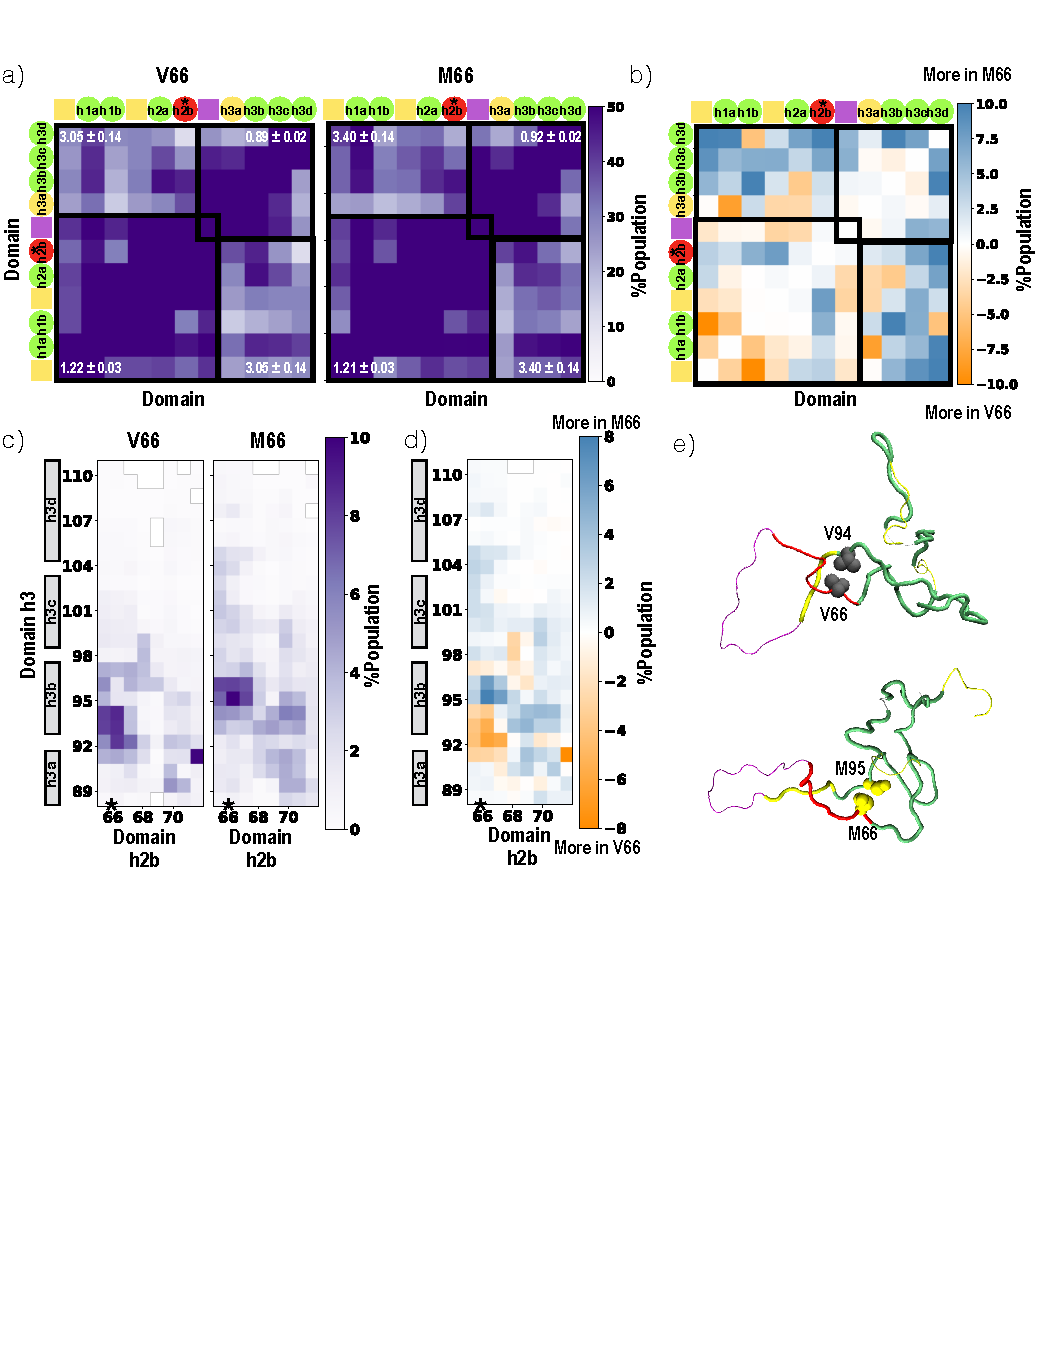
\includegraphics[width=0.7\textwidth,trim={0 0cm 0 0cm},clip]{./figures/fig4.pdf}
\caption{{\bf \DIFadd{Blob hydrophobicity and charge properties for SNPs in aggregating proteins.}} \DIFadd{a) Distribution of \chargechar{}es (Das-Pappu\mbox{%DIFAUXCMD
\cite{Das2013} }\hspace{0pt}%DIFAUXCMD
phase) across the SNP dataset, for each blob \hydrochar. Possible values of the blob \chargechar{} are 1 (Weak polyampholyte), 2 (Janus or boundary region), 3 (Strong polyampholyte), 4 (Negatively-charged strong polyelectrolyte), and 5 (Positively-charged strong polyelectrolyte). b-c) Fraction of \nSNPs or \dSNPs that are found in blobs of each \hydrochar{} (b) or \chargechar{} (c) in non-aggregating (nAgg) proteins and known-aggregating (Agg) proteins. Panels a-c used whole sequence blobulation ($\Ht=0.4, \Lmin=4$); error bars represent one standard error for multinomial distributed data. Division of nAgg and Agg proteins is described in Methods. d) Enchriment of dSNPs binned by threshold $\Ht$ and length $L$ of the SNP-containing blob, calculated using unconstrained-length blobulation as in Figure \ref{blob_vs_window}D, but separated by aggregation tendency. Black lines are to guide the eye.}}
\label{agg_enrich} 
\end{SCfigure*}

\subsection*{\DIFadd{Disease-associated SNPs are enriched for mutations that change local blob characteristics and overall protein blob topology}}
\DIFadd{Whole-sequence }\DIFaddend blobulation \DIFdelbegin \DIFdel{process }\DIFdelend yields a series of \DIFdelbegin \DIFdel{h blobs}\DIFdelend \DIFaddbegin \DIFadd{h-blobs}\DIFaddend , connected by \DIFdelbegin \DIFdel{p and s linkers}\DIFdelend \DIFaddbegin \DIFadd{p- and s-blobs}\DIFaddend , which we term the ``blobular topology\DIFdelbegin \DIFdel{"}\DIFdelend \DIFaddbegin \DIFadd{''}\DIFaddend . Such a topology is analogous to the classic protein topology of secondary structure elements\DIFaddbegin \DIFadd{, although the location of edges and number of elements may be distinct}\DIFaddend . A SNP can alter the blobular topology by moving a short stretch of contiguous residues above or below the minimum blob size, either forming a new small h-blob or dissolving an existing small h-blob respectively. \DIFaddbegin \DIFadd{A SNP can also split a long h-blob by interrupting a long contiguous hydrophobic sequence, or merge two smaller h-blobs into one long h-blob by removing such an interruption. 
}

\DIFadd{Here we tested whether the \dSNPs were more likely to change the topology determined by whole-sequence blobulation ($\cmin=0.4, \Lmin=4$). Figure \ref{c3_h_p_enrich}A displays the fraction of \nSNPs and \dSNPs that cause each of type of topological change. }\DIFaddend In the background case we expect to see more formation than dissolution, since the blob \DIFdelbegin \DIFdel{frequency }\DIFdelend \DIFaddbegin \DIFadd{count }\DIFaddend decreases with length (Figure \ref{blob_vs_window} \DIFdelbegin \DIFdel{e}\DIFdelend \DIFaddbegin \DIFadd{h}\DIFaddend ), and there are more blobs just below the minimum length than just above it. Figure \ref{c3_h_p_enrich}A confirms this expectation for \DIFdelbegin \DIFdel{\nSNPs. A SNP can also split a long h-blob by interrupting a long contiguous hydrophobic sequence, or merge two smaller h-blobs into one long h-blob by removing such an interruption. Using the mild hydrophobicity threshold of 0.4 and minimum blob length of 4 residues, fewer than 15\% of SNPs overall cause a topological change. As shown in Figure \ref{c3_h_p_enrich}C, however, certain topological changes are strongly enriched in \dSNPs. %DIF <  reveals the fraction of \nSNPs and \dSNPs that cause one of these four possible changes in blobular topology
While }\DIFdelend \DIFaddbegin \DIFadd{nSNPs, and }\DIFaddend the difference between the fraction of \nSNPs and \dSNPs that form \DIFaddbegin \DIFadd{new }\DIFaddend h-blobs is not significant  (\DIFdelbegin \DIFdel{$p>10^{-3}$), }\DIFdelend \DIFaddbegin \DIFadd{$P>10^{-3}$). 
}

\DIFadd{Other topological changes, however, are strongly enriched in dSNPs. As shown in Figure \ref{c3_h_p_enrich}A, }\DIFaddend \dSNPs are significantly more likely to dissolve h-blobs (\DIFdelbegin \DIFdel{$p<10^{-21}$}\DIFdelend \DIFaddbegin \DIFadd{$P<10^{-21}$}\DIFaddend ), split h-blobs (\DIFdelbegin \DIFdel{$p<10^{-80}$}\DIFdelend \DIFaddbegin \DIFadd{$P<10^{-80}$}\DIFaddend ), and merge h-blobs (\DIFdelbegin \DIFdel{$p<10^{-36}$}\DIFdelend \DIFaddbegin \DIFadd{$P<10^{-36}$}\DIFaddend ). The magnitude of enrichment (2.1-fold) is greatest for SNPs that split longer h-blobs into two shorter ones and is only moderately weaker for the reverse merging of two h-blobs (1.7-fold). These results are consistent with the functional sensitivity of long blobs shown in Figure \ref{blob_vs_window}\DIFdelbegin \DIFdel{c. }%DIFDELCMD < 

%DIFDELCMD < %%%
%DIF < In this section we focus on the differences in the length of h-blobs surrounding each SNP between the reference and the alternative allele. \matt{provide motivation for hypothesis somewhere in here} We hypothesize that \dSNPs should show a larger difference in the h-blob lengths between the reference and alternative alleles, compared to the differences induced by \nSNPs. For concreteness we only consider h-blob lengths as computed at the hydrophobicity threshold $\hydrothresh=0.4$. 
%DIF < In addition to topological changes, SNPs can also affect blob length by shifting blob boundaries while preserving the sequential order of h-, p-, and s- blobs. For this analysis we fix the hydropathy threshold to $c=0.4$ with minimum h-blob size $n_{\rm min}=4$. We consider all SNPs that don't alter the blob topology and for which at least one of the two alleles is in an h-blob. For this set of SNPs we can unambiguously assign one h-blob to each SNP. We then compute the length of the h-blob for the reference and the alternative allele. The change in blob length is defined as $\Delta = L_{\rm alt} - L_{\rm ref}$. As shown in Figure \ref{c3_h_p_enrich}C, nSNPs show little or no significant deviation from zero net change in direction, $\langle {\rm Sign}[\Delta]\rangle \approx 0$. This suggests a genome-wide steady-state in the h-blob lengths, where alternative and reference alleles have no net bias towards residing in longer or shorter h-blobs. However, dSNPs show a clear bias towards the alternative allele residing in shorter h-blobs. For disease-associated SNPs the alternative allele is almost always the risk-conferring allele. Therefore we find that disease-associated alleles have a significant tendency to shorten h-blobs that are long in the reference genomic state. The fact that the alternative alleles show a systematic bias towards shorter h-blobs is another sign that some hydrophobic blobs are being maintained at longer lengths than background genetic variation would create.
%DIFDELCMD < 

%DIFDELCMD < %%%
%DIF < \grace{MATT can revisit these two paragraphs? Suggestion: Shorten them and reduce redundancy with information from figure c.  If you can clarify which information is consistent with panel c and then focus on information that panel C doesn't have I think that will help.}
%DIF < \matt{I wrote a mock pp that would be suitable for a revised analysis where we just consider the topology-preserving SNPs. If we do this, then I think we can just show the change-of-direction results in the Figure. That would be enough to make the key points. The quantitative length changes are better explained by the topology-changing SNPs and existing barcharts in the Figure. }
%DIF < \matt{ok, i think we decided to remove this analysis.}
%DIF < In addition to topological changes, SNPs can also affect blob length by shifting blob boundaries. %Quantitative changes in h-blob lengths induced by nSNPs and dSNPs supports the enrichments observed for categorical changes to blob topology. Figure \ref{c3_h_p_enrich}D shows the average blob length changes induced by the polymorphisms, where we split the length change into the direction and the magnitude. We define $\Delta = L[{\rm Alt}] - L[{\rm Ref}]$ as the difference in h-blob length for each SNP between the alternative and reference alleles. Taking $I=\Delta/|\Delta|\in\{-1,1\}$ as the indicator variable for direction of length change for each SNP, the average $\langle I \rangle$ is shown in the top of Figure \ref{c3_h_p_enrich}D). This can be converted to the proportion of SNPs $x$ where the alternative allele has a longer h-blob: $x=(1+\langle I \rangle)/2$. As shown in Figure \ref{c3_h_p_enrich}C), \nSNPs and \dSNPs show a different pattern for the change in direction across the range of h-blob sizes. For all blob lengths, nSNPs show little or no significant deviation from zero net change in direction, $\langle I \rangle \approx 0$. This suggests a genome-wide steady-state in the h-blob configuration, where alternative and reference alleles have no net bias towards residing in longer or shorter h-blobs. Conversely, dSNPs show a clear bias towards the alternative allele residing in shorter h-blobs, especially for longer h-blobs. In the largest h-blob length bin we find that $\langle I \rangle \approx -0.1$ for \dSNPs, corresponding to about $45\%$ of the alternative alleles having longer h-blobs than reference allele. For disease-associated polymorphisms the alternative allele is the risk-conferring allele. Therefore we find that disease-associated alleles have a significant tendency to shorten h-blobs that are long in the reference genomic state. The fact that the alternative alleles show a systematic bias towards shorter h-blobs is another sign that some hydrophobic blobs are being maintained at longer lengths than background genetic variation would create.
%DIF < 
%DIF < In terms of the magnitude of the length change induced by a polymorphism there is also a clear difference between \nSNPs and \dSNPs, as shown in Figure \ref{c3_h_p_enrich}b). For \nSNPs there is a trend towards larger length changes for longer h-blobs up to a blob size around $L\sim 40$, at which point the trend reverses and the length changes become smaller for larger h-blobs. We interpret this pattern to mean that for the longest h-blobs, \nSNPs are biased towards SNPs that do not change the blob length. In contrast, the trend for \dSNPs is similar to \nSNPs up to blob lengths $L\sim 40$, albeit with a slight increase in the magnitude of change compared to \nSNPs for each bin. However, for $L\geq 40$ the blob length changes induced by \dSNPs continues to increase with the blob size. This accords with the interpretation that long h-blobs are functional and therefore SNPs that cause large changes in long h-blobs are much more likely to be classified as a \dSNP than an \nSNP. In turn, this supports the broad findings of this study that some \dSNPs are disease-associated due to their impact on their surrounding hydrophobic blobs. 
%DIFDELCMD < 

%DIFDELCMD < %%%
\DIFdelend \DIFaddbegin \DIFadd{D. }\DIFaddend Regardless of overall topological changes, SNPs may change the characteristics of their local blob. Such changes may affect blob topology (as in Figure \ref{c3_h_p_enrich}\DIFdelbegin \DIFdel{a}\DIFdelend \DIFaddbegin \DIFadd{A}\DIFaddend ), or simply shift blob boundaries\DIFdelbegin \DIFdel{(as in Figure \ref{c3_h_p_enrich}b). We now broaden the analysis to include changes in blob characteristics that do not necessarily affect the blob boundaries. %DIF < Pure classification transitions will be far more common in shorter blobs, where each residue contributes more to the overall blob assignment. 
%DIF < In order to further test the significance of blob characteristics in distinguishing functional variation, we evaluated the enrichment of dSNPs for difference in blob characteristics of original SNP blob and mutated SNP blob. 
%DIF < For blob \hydrochar{}, the difference between the original SNP blob and the mutated SNP blob can have two outcomes: (i)  the blob assignment changes; resulting in a h $\rightarrow$ p blob or p $\rightarrow$ h blob ii) the blob assignment does not change; resulting in a h $\rightarrow$ h or p $\rightarrow$ p blob. 
}\DIFdelend \DIFaddbegin \DIFadd{, causing a transition in blob class at the site of the SNP. The latter case is included in the data in Figure \ref{c3_h_p_enrich}B. }\DIFaddend We observe that about 17\% of the \nSNPs and 22\% of \dSNPs introduce a blob-\hydrochar{} change \DIFaddbegin \DIFadd{at the site of the SNP}\DIFaddend , yielding a 1.3 fold enrichment \DIFdelbegin \DIFdel{for blob ~\hydrochar{} changes (}\DIFdelend \DIFaddbegin \DIFadd{($P<10^{-10}$, }\DIFaddend Fig~\ref{c3_h_p_enrich}\DIFdelbegin \DIFdel{b). %DIF < We calculated the frequency of each of the four possible  blob-\hydrochar{} transitions: h $\rightarrow$ p, h $\rightarrow$ h, p $\rightarrow$ h, and p $\rightarrow$ p (Fig~\ref{c3_h_p_enrich}b). 
Fig~\ref{c3_h_p_enrich}c compares the frequency of possible }\DIFdelend \DIFaddbegin \DIFadd{B). Figure ~\ref{c3_h_p_enrich}C compares the rates of specific }\DIFaddend blob \hydrochar{} transitions. Mutations involving h $\rightarrow$ p blob transitions yield the maximum enrichment (1.5 fold\DIFaddbegin \DIFadd{, $P<10^{-10}$}\DIFaddend ) among \dSNPs. %DIF < suggesting a particularly high likelihood of functional impact upon introduction of a less hydrophobic residue in a generic hydrophobic sequence (for example, introduction of a charged residue into a buried position). %, and constitute only 6\% of the total dataset. 
%DIF < These results suggest a particularly 
In contrast, \dSNPs are only 1.1 fold enriched \DIFaddbegin \DIFadd{($P<10^{-3}$) }\DIFaddend in the reverse \DIFdelbegin \DIFdel{transition (}\DIFdelend p $\rightarrow$ h \DIFdelbegin \DIFdel{)}\DIFdelend \DIFaddbegin \DIFadd{blob transition}\DIFaddend , and SNPs that remain in \DIFdelbegin \DIFdel{p blobs }\DIFdelend \DIFaddbegin \DIFadd{p-blobs }\DIFaddend for both the ancestral and derived allele \DIFdelbegin \DIFdel{in p blobs }\DIFdelend are depleted among disease-associated SNPs. 
%DIF < Previously, in disordered proteins, analogous to blob transitions, disorder $\rightarrow$ order or order $\rightarrow$ disorder transitions due to \dSNPs SNP has been observed~\citep{Vacic2012a, Uversky2014b}.
%DIF < 
%DIF < In structured proteins enrichment or depletion of h blobs could potentially effect the folding core or the kinetics of binding core. 
%DIF < It has been found that these transitions frequently disrupt MoRFs in disordered proteins. Because MoRFs mediate protein-protein interactions, it follows that protein interaction networks may also be disrupted~\citep{Uversky2014b}. 
%DIF < Mutations that reverse residue charge would be expected to have particularly strong functional effects, but would not affect the blob \hydrochar{}. They could, however, affect the blob \chargechar{}. Mutations involving a neutral residue and a charged residue could also affect the blob \chargechar{}. These changes can occur either directly, by changing the fraction of positive/negative residues in the original blob or indirectly, by affecting the blob segmentation.   %or could also the difference between the original SNP blob and mutated SNP blob can have two outcomes (Fig~\ref{blob_transition}c):  (i) it can change the blob \chargechar{} class due to direct or indirect effect a) SNP can directly increase or decrease the fraction of charged residue (FCR) in a blob due to gain or loss of a charged amino acid. This can move the blob into a new region in the Das-Pappu classification ~\citep{Das2013} b) SNP changes the blob \hydrochar{} or blob length, indirectly resulting in a change in blob \chargechar{}. ii) it does not change the blob \chargechar{}, resulting in no change (Fig~\ref{blob_transition}c). 
%DIF < We find that about 79\% of the \nSNPs and 70\% of \dSNPs do not cause any blob-\hydrochar{} transition in either \dSNPs and \nSNPs. In line with the above blob-\hydrochar{} observations \dSNPs are 1.3 fold enriched when blob \chargechar{} change is present.
%DIF < We further zoomed into the fraction and enrichment in each case of blob \chargechar{} transition 

Similarly, the frequency of SNP-induced changes in blob \chargechar{} is shown in \DIFdelbegin \DIFdel{Fig~\ref{c3_h_p_enrich}c}\DIFdelend \DIFaddbegin \DIFadd{Figure ~\ref{c3_h_p_enrich}C}\DIFaddend , for transitions \DIFdelbegin \DIFdel{involving blobs in categories }\DIFdelend \DIFaddbegin \DIFadd{between blobs in class }\DIFaddend 1 \DIFdelbegin \DIFdel{, }\DIFdelend \DIFaddbegin \DIFadd{(weak polyampholyte), class }\DIFaddend 2 \DIFdelbegin \DIFdel{, and 3. %DIF <  (weak polyampholyte), category 2 (Janus), or category 3 (strong polyampholyte). 
%DIF < Frequency and disease enrichment broken down by wildtype blob \hydrochar~ and mutant blob \hydrochar~ are shown in Fig~\ref{blob_transition}d, for blobs in category 1 (weak polyampholyte), category 2 (Janus), or category 3 (strong polyampholyte). 
Transitions involving categories }\DIFdelend \DIFaddbegin \DIFadd{(Janus), or class 3 (strong polyampholyte). Transitions involving classes }\DIFaddend 4 or 5 (positively or negatively-charged strong \DIFdelbegin \DIFdel{poly electrolyte}\DIFdelend \DIFaddbegin \DIFadd{polyelectrolytes}\DIFaddend ) represented fewer than 1.5 \% of the total transitions. Disease-associated SNPs are enriched for all mutations that change blob \chargechar{} and either \DIFdelbegin \DIFdel{unenriched }\DIFdelend \DIFaddbegin \DIFadd{un-enriched }\DIFaddend or weakly depleted for mutations that do not change the local blob \chargechar. %DIF < increased with the severity \grace{word choice} of the transition, 
\DIFdelbegin \DIFdel{so $1\rightarrow 3> 1 \rightarrow 2$ and $3\rightarrow 1 > 3\rightarrow 2$. %DIF < Disease-associated SNPs are most strongly enriched (1.7 fold) for SNPS that switch a weak polyampholyte (1) blob to a strong polyampholyte (3) blob were the most strongly enriched for disease-association. 
}\DIFdelend Collectively, these results are consistent with the increased mutational sensitivity of hydrophobic (and typically buried) blobs that is shown in Figure \ref{blob_vs_window}\DIFaddbegin \DIFadd{D}\DIFaddend , while also emphasizing that mutations that \emph{change} \chargechar{} are particularly likely to be causal. For instance, charge reversal of a charged residue could have particularly strong functional effects. While these effects might be amplified if the \DIFdelbegin \DIFdel{residue was located in an }\DIFdelend \DIFaddbegin \DIFadd{charged residue was in a weak }\DIFaddend h-blob (\DIFaddbegin \DIFadd{a possibility explained in Methods) }\DIFaddend and thus interacting with other protein residues\DIFdelbegin \DIFdel{)}\DIFdelend , the charge reversal itself would not affect the blob \hydrochar{}.  
%DIF <    These trends are consistent with evidence that the severity of a SNP on protein function is moderately correlated with the physicochemical difference between the original amino acid and the missense variant, which is often exploited in  commonly-used SNP effect predictors ~\citep{Stone2005, Kumar2009, Tang2004}.
%DIF < \grace{Can we make this statement stronger, use more recent reference?}  % $1\rightarrow 3>1\rightarrow 2\sim 3\rightarrow 1 > 2\rightarrow 3\sim 2\rightarrow 1>3\rightarrow 2.   We find that all blob \chargechar{} transitions are enriched. % whereas no transitions either show no enrichment or depletion. This indicates that amino-acid substitution that affect blob \chargechar{} potentially affect protein function. 
%DIF < While generic transitions of blob \hydrochar{} or \chargechar{} yield an equivalent amount of enrichment (1.3 fold) for disease-association, more SNPs in the present dataset induce a blob \chargechar{} transition than a \hydrochar{} transition (29\% vs 22\%, respectively). Furthermore, \chargechar{} distinguishes between lower and higher enrichment transitions, since most 1$\rightarrow$ 2 mutations (1.4 fold enrichment) and 1$\rightarrow$ 3 mutations (1.7 fold enrichment) will also count as h$\rightarrow$ p mutations (1.5 fold enrichment).This result suggests that for SNPs that change the blob \hydrochar{}, a further split into those with weaker or stronger effects on \chargechar{} provides greater resolution of functional effects. Mutations that reverse residue charge would be expected to have particularly strong functional effects, but would not affect the blob \hydrochar{}. 
%DIF < These results suggest that transitions in blob ~\chargechar{} may be particularly useful for predicting whether variants have a functional effect.
 %DIF < From this we conclude that for segmentation based on \hydrochar{}, 

%DIF < a maximum enrichment observed in blob \chargechar{} is higher than for \hydrochar{} (1.8 fold for 1 $\rightarrow$ 3 vs 1.6 fold for h $\rightarrow$ p).  
\DIFaddbegin \ifnum\value{\DIFadd{includefigs}}\DIFadd{>0 }{
\begin{figure}[!ht]
\center
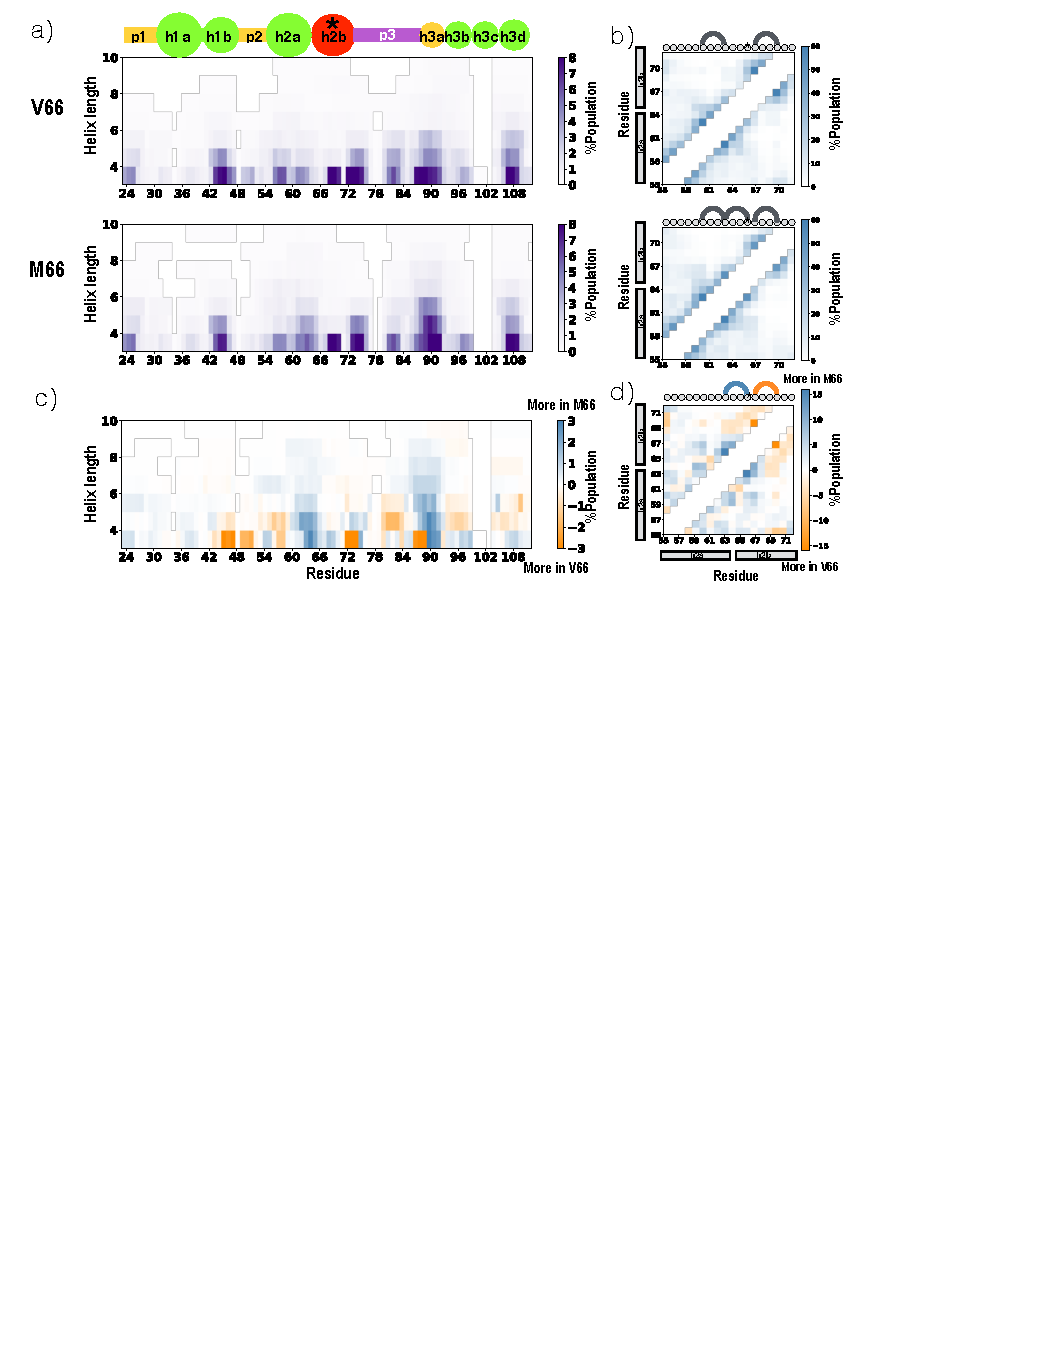
\includegraphics[width=\linewidth,trim={0 0cm 0 0cm}]{./figures/fig5.pdf}
\caption{{\bf \DIFaddFL{Distribution of SNPs that change blob properties}}  \DIFaddFL{a) Fraction of \nSNPs or \dSNPs that change the blobular topology by either forming or dissolving an h-blob or by splitting one h-blob or merging two h-blobs. b) Fractions of \nSNPs or \dSNPs that induce a change in \hydrochar{} or \chargechar.  c) The enrichment of \dSNPs relative to \nSNPs that induce a specific transition between the blob containing the reference allele (x-axis) and the blob containing the alternative allele (y-axis). This is shown for two blob properties, \hydrochar{} (left) and \chargechar{} (right), where the \chargechar{} categories are the same as in Figure 4. d) The overall proportion of \nSNPs that induce each of the blobular topology transitions shown in c).  Fewer than 1.5\% of SNPs involve charge classes 4 or 5, and these data are not shown for readability. Significant enrichment or depletion in \dSNPs is annotated with one star ( $P< 10^{-3}$) or two stars ($P< 10^{-10}$). Errors bars in (a) and (b) represent one standard error for multinomial (a) or binomial (b) distributed data. All panels use whole sequence blobulation ($\Ht=0.4$ and $\Lmin=4$).}}
\label{c3_h_p_enrich} 
\end{figure}
}\fi
\DIFaddend 

%DIF < To summarize, we find that difference in Wild Type and SNP blob characteristics is somewhat positively correlated with the functional impact of the SNP. 
%DIF < the enrichment between presence and absence of transitions for \dSNPs is very clear, blob class transitions are enriched whereas no transitions either show no enrichment or depletion whereas the same is not true for blob type transitions. 
%DIF < \ruchi{There is evidence that the severity of a SNP on protein function is somewhat correlated with the physicochemical difference between the original amino acid and the missense variant ~\citep{Stone2005}. This is in line with previous evidence of correlation between the severity of the SNP and physicochemical difference between original and SNP residue. } comment: move to discussion
%DIF < \subsection*{Disease-associated SNPs have a larger impact on blob lengths than non-disease-associated SNPs for the longest h-blobs}
%DIF < \begin{figure}[!ht]
%DIF < \includegraphics[scale=1,width=0.5\textwidth,trim={0 0cm 0 0cm},clip]{./figures/blob_length_changes.pdf}
%DIF < \caption{{\bf Change in h-blob lengths $\Delta$ induced by polymorphisms} Panels a) and b) show the average change in h-blob lengths between the reference and alternative allele, binned by the h-blob length. For each blob length bin, we compute the averages using the h-blob length for the reference and alternative alleles separately, and then take the mean of those two values. We only consider h-blob lengths as defined at the hydrophocity threshold of $c=0.4$. Each bin has a minimum of 10 SNPs. a) The average change in direction in the h-blob length, with ``+1'' corresponding to the alternative allele having a longer h-blob than the reference allele, and conversely for ``-1''. b) The average magnitude of change in h-blob length.\matt{change to Sign[Delta]}}
%DIF < \label{fig:blob_length_changes} 
%DIF < \end{figure}
%DIF < For both SNP categories the alternative allele resides in the shorter h-blob compared to the reference allele, on average. For example, for the smallest h-blob bin $\langle I \rangle \approx -0.6$ for \dSNPs, which corresponds to $\approx 20\%$ of the SNPs having a longer h-blob for the alternative allele compared to the reference. Moreover, we find that the alternative allele in larger h-blobs are more likely to shorten the blob compared to the alternative allele in shorter h-blobs. In the largest h-blob length bin we find that $\langle I \rangle \approx -0.9$ for both \nSNPs and \dSNPs, corresponding to only about $5\%$ of the alternative alleles having longer h-blobs than reference allele. The fact that the alternative alleles show a systematic bias towards shorter h-blobs is another sign that hydrophobic blobs are being maintained at longer lengths than background genetic variation would create. 
\DIFdelbegin \section{\DIFdel{Discussion}}
%DIFAUXCMD
\addtocounter{section}{-1}%DIFAUXCMD
\DIFdelend \DIFaddbegin \section*{\DIFadd{Discussion}}
\DIFaddend In the present work, we have presented the ``blobulation'' scheme for identifying interaction-rich protein regions from sequence, and tested its use in detecting functional modules across the proteome. %DIF < We found that disease-associated mutations are weakly enriched (1.15 fold) in blobs that are hydrophobic by the weak criteria we had previously\cite{Lohia2019} used for intrinsically disordered proteins. 
\DIFdelbegin \DIFdel{We }\DIFdelend \DIFaddbegin \DIFadd{We show that hydrophobic h-blobs in solvated proteins are more likely to be buried: the h-blob SASA is 60\% that of non h-blobs. H-blobs are also nearly twice as likely to contain $\beta-$strands, supporting their proposed role as tertiary interaction-sites. We }\DIFaddend find that enrichment of disease-associated mutations in hydrophobic blobs increases with the strictness of the hydrophobic blob criteria, with greater than 4-fold enrichment for disease-association in the longest, most hydrophobic blobs. \DIFaddbegin \DIFadd{This result persists when SNPs in transmembrane domains are removed from the analysis. }\DIFaddend The range and resolution of varying enrichment is strongly damped in the {\it status quo} fixed-length moving window approach. Stratifying SNPs by their surrounding blob properties reveals genome-wide differences in blob genetic diversity, demonstrating pervasive differential selection on at least some classes of blobs. 
\DIFaddbegin \DIFadd{This observation supports our hypothesis that blobulation provides a more meaningful and less noisy approach to protein segmentation than use of a fixed-length moving window.
}\DIFaddend 

We also find that disease-associated mutations are significantly more likely than non-disease associated mutations to change the topology of the sequence.  This suggests that blobulation provides a meaningful topology that can be used as a framework for sequence analysis, and which requires only the protein amino acid sequence and two parameters (minimum blob length and hydrophobicity threshold). Once blobs are identified, they can be characterized \DIFdelbegin \DIFdel{on }\DIFdelend \DIFaddbegin \DIFadd{using }\DIFaddend any property of interest. As an example, in the present work, we \DIFdelbegin \DIFdel{also }\DIFdelend find that disease-associated mutations are moderately enriched for mutations that cause transitions in blob~\hydrochar{} (up to 1.5 fold) and strongly enriched for mutations that cause certain transitions in blob~\chargechar{} (1.7 fold).
%DIF < The present results also support a fundamental role for hydrophobicity in determining the sensitivity of a given protein region to disease-causing mutations. 

%DIF < All protein level methods for variant-to-function prediction rely on some form of residue characterization. In addition to physicochemical properties~\citep{Stone2005, Niroula2015, LopezFerrando2017,Hecht2015,Popov2019} similar to the \hydrochar{} and \chargechar{} considered in the present work, these may include evolutionary conservation~\citep{Stone2005, Thomas2004, Ng2001, Choi2012, Hecht2015, Niroula2015,Thomas2004,Capriotti2006} and structural propensities~\citep{Iqbal2020, Ittisoponpisan2019, Capriotti2004,Capriotti2005, Parthiban2006, Wainreb2010,Popov2019}. Our present results suggest that blob-level characterization may provide a generally useful framework for most such analyses.  
%DIF < Methods relying on physiochemical properties are uniquely suited for application to disordered sequences and weakly conserved sequences, and may be compared directly against {\it in vitro} experimental results for mechanistic consistency. Yet many are still limited by a reliance on structural information for predictive accuracy. 
%DIF <  Disease-associated mutations are moderately enriched for mutations that cause transitions in blob~\hydrochar{} (up to 1.5 fold) and strongly enriched for mutations that cause certain transitions in blob~\chargechar{} (1.7 fold).
\DIFdelbegin %DIFDELCMD < 

%DIFDELCMD < %%%
\DIFdelend While we are not aware of a similar approach applied to generic proteins, hydrophobic blobs are analogous to the aggregation ``hot spots" identified by tools such as AGGRESCAN~\citep{ConchilloSole2007}, ProA~\citep{Fang2013}, and Zyggregator~\citep{Tartaglia2008}. 
We do find that functional sensitivity in aggregating proteins follows similar trends \DIFaddbegin \DIFadd{as in non-aggregating proteins, }\DIFaddend but emerges in shorter blobs satisfying weaker hydrophobicity criteria. The difference between aggregating and generic proteins is thus quantitative, not qualitative, and demonstrates that hydrophobic interactions occur on a useful continuum. 
%DIF <  \dSNPs in aggregating proteins are enriched for weakly hydrophobic blobs, while SNPs in strongly hydrophobic blobs are not found in such proteins.

%DIF < These results support the use of blobulation as a simple method for segmenting proteins, requiring only the protein amino acid sequence and two parameters (minimum blob length and hydrophobicity threshold). Once blobs are identified, they can be characterized on any property of interest, including  mean hydrophobicity, net charge per residue, fraction of polar residues, fraction of disordered residues, etc. The present results also support a fundamental role for hydrophobicity in determining the sensitivity of a given protein region to disease-causing mutations. 
\DIFdelbegin %DIFDELCMD < 

%DIFDELCMD < %%%
%DIF < These segments (also referred to as blobs) define the 'local sequence' for a residue more effectively than the moving window approach most commonly used in sequence-only methods.  Blobulation is a simple method requires only the protein's primary sequence, along with two parameters of minimum blob length and threshold. Once the blobs are identified, they can be characterized on any property of interest such as mean hydrophobicity, net charge per residue, fraction of polar residues, etc. Blobulation and blob characterization are especially meaningful for long protein sequences. The average property of a long protein is insensitive to a single residue change. However, the identified blobs are more likely to be sensitive to this change. 
%DIFDELCMD < 

%DIFDELCMD < %%%
%DIF < For both nSNPs and dSNPs it is evident that $H$ varies with $c$. For both nSNPs and dSNPs, therefore, the heterozygosity pattern indicates that blobulation identifies functional protein elements, at least in a genome-wide enrichment sense. Given that the proxy for functionality that we use are SNPs strongly associated with severe genetic diseases, it suggests that hydrophobic blobs are critical functional objects in many proteins. 
%DIFDELCMD < 

%DIFDELCMD < %%%
\DIFdel{Structural data implicitly provides insight into the segmentation of a protein sequence, but we show here that segmentation may be meaningfully estimated from the sequence alone. %DIF < Based on the present results, we suggest that structureless methods may recapture some accuracy of structure-based methods by introducing sequence-based segmentation.  
}\DIFdelend We have proposed blobulation as a generalizeable approach for segmentation, although in principle, secondary structure prediction could be used instead. \DIFdelbegin \DIFdel{For many proteins}\DIFdelend \DIFaddbegin \DIFadd{As demonstrated by the example of ubiquitin (Figure \ref{cartoon}E)}\DIFaddend , however, \DIFdelbegin \DIFdel{this approach }\DIFdelend \DIFaddbegin \DIFadd{secondary structure elements can cross between different faces of the protein, so secondary structure boundaries may not capture functional boundaries. Moreover, for many proteins, the use of secondary structure }\DIFaddend would be frequently unfeasible and overly restrictive. In addition to the challenges inherent in predicting secondary structure (which may be highly sensitive to the local protein environment or simply non-existent), many secondary structure prediction methods require alignment to a homologous sequence with known structure~\citep{Yang2018, Zhang2018a,Wang2017,Ma2018}. This is essential for secondary structure predictors to achieve their primary goal: \DIFdelbegin \DIFdel{distinguishing }\DIFdelend \DIFaddbegin \DIFadd{determining }\DIFaddend \textit{\DIFdelbegin \DIFdel{between}\DIFdelend \DIFaddbegin \DIFadd{which}\DIFaddend } secondary \DIFdelbegin \DIFdel{structures}\DIFdelend \DIFaddbegin \DIFadd{structure the segment will adopt}\DIFaddend . Segmentation, however, only requires knowing where the segment begins and ends.  

\DIFdelbegin \DIFdel{We anticipate that these results may further efforts to assess functional significance of SNPs for which disease-causality is uncertain.  Despite the wealth of genetics information presently available, %DIF < (gnomAD~\citep{Karczewski2019},OMIM~\citep{McKusick2007},ClinVar~\citep{Landrum2018}), 
the complex nature of many phenotypes makes the }\DIFdelend \DIFaddbegin \DIFadd{Information about the hydrophobic blob context of a SNP should also aid the }\DIFaddend identification of \DIFdelbegin \DIFdel{causal variants difficult~\mbox{%DIFAUXCMD
\citep{Claussnitzer2020}}\hspace{0pt}%DIFAUXCMD
. SNP-prediction methods often test residue properties for relevance by machine learning algorithms, %DIF <  such as neural networks~\citep{Bromberg2007, Hecht2015, LopezFerrando2017}, Hidden Markov Models~\citep{Thomas2004,Shihab2012}, Random forests~\citep{Niroula2015, Wainreb2010} or Support vector Machines~\citep{Yue2005,Rentzsch2018,Calabrese2009,Capriotti2006}). 
}\DIFdelend \DIFaddbegin \DIFadd{functional mutations. In the context of interpreting Genome-Wide-Association (GWAS) results \mbox{%DIFAUXCMD
\citep{Gallagher2018}}\hspace{0pt}%DIFAUXCMD
, the blob characteristics surrounding an associated variant provides metrics for fine-mapping and ranking putative causal variants. Such blob metrics could also be used as input features for predicting variant function with machine-learning algorithms, }\DIFaddend which derive their decision rules based on training datasets of annotated mutations\DIFdelbegin \DIFdel{, and therefore are sensitive to the training set used. Machine learning methods also rely on a large number of features, which can obscure the biological relevance of any given feature. Here we have both performed hypothesis-driven tests for enrichment of certain features in putatively causal SNPs and %DIF < , based on the principle that those features that are most relevant for evaluating SNPs should be detectable by simple enrichment tests. 
%DIF < Widely used methods to find genotype/phenotype associations, such as pedigree-based linkage studies or population-based association studies, have identified thousands of associations with a wide spectrum of phenotypes and diseases~\citep{Buniello2019, Gallagher2018, Tam2019}. 
%DIF < Association of a SNP with a disease does not necessarily indicate  causality,~\citep{Boyle2017, Goldstein2009, McClellan2010,MacArthur2014}  %For example, alleles that happen to be in strong linkage disequilibrium with causal variants will also show statistical association. Other lines of evidence are often needed to identify or prioritize likely functional variants, 
%DIF < motivating the development multiple complementary approaches for predicting the functional effects of SNPs. 
provided }\DIFdelend \DIFaddbegin \DIFadd{. To this end, we provide }\DIFaddend a two-dimensional table (\DIFdelbegin \DIFdel{Dataset 1) of wide-ranging enrichments }\DIFdelend \DIFaddbegin \DIFadd{SI Dataset 2) of disease-association enrichment }\DIFaddend as a function of blob properties\DIFdelbegin \DIFdel{, which can be used as inputs in future predictions}\DIFdelend .

%DIF < If hydrophobic blobs have served a functional role over evolutionary timescales, then their DNA sequences are expected to show evidence of selection in order to maintain the relevant hydrophobic properties. Additionally, if hydrophobic blobs provide subdomains of high domain-domain and domain-membrane interactions, we may expect an enrichment of functional SNPs under selection. One consequence of selection over a genomic region is a distortion in the genetic diversity present in that region compared to neutrally evolving parts of the genome \cite{mcvicker_2009,lohmueller_2011}. Here we only consider genetic diversity as measured by the population heterozygosity, $H\equiv 2\nu(1-\nu)$, where $\nu$ is the frequency of the coded allele. Any genome-wide difference in $H$ between different types or categorizations of genomic regions is a signal of differential selection between these types of regions. As selection only operates on regions of the genome that are functional or linked to functional variation, observing significant differential heterozygosity is a strong indicator that the categorization is stratifying functional regions. Here we found compelling evidence from population genetic data that, on average, SNPs in highly hydrophobic blobs are under differential selection relative to SNPs in other blobs. We find that non-disease associated sNPs in highly hydrophobic blobs show signature of greater balancing selection. Conversely, we find that disease-associated SNPs in highly hydrophobic blobs show signature of greater purifying selection. Overall these findings show that, based on distortions in the population genetic diversity, highly hydrophobic blobs are enriched for SNPs under selection.
\DIFaddbegin \DIFadd{Many of the analyses in this manuscript use the relaxed criteria for h-blobs to demonstrate that even conservative stratification yields meaningful differences. Thus, the potential applications are not limited to those residues that meet the strict criteria or have the strongest disease-association. We view the parameter sensitivity of blobulation as a methodological strength, because adjusting the two parameters allows the user to ``zoom'' in or out by tuning the number of detected edges. In our parallel development of a blobulation graphical interface (see Methods for access information), we have repeatedly observed that such tuning can bring previously-obscured sequence organization into visual focus.  
}\DIFaddend 

%DIF < SNP-prediction methods often test residue properties for relevance by machine learning algorithms such as neural networks~\citep{Bromberg2007, Hecht2015, LopezFerrando2017}, Hidden Markov Models~\citep{Thomas2004,Shihab2012}, Random forests~\citep{Niroula2015, Wainreb2010} or Support vector Machines~\citep{Yue2005,Rentzsch2018,Calabrese2009,Capriotti2006}). The machine learning methods derive their decision rules based on training datasets of annotated mutations, and therefore are sensitive to the training set used. Machine learning methods also rely on a large number of features, which can obscure the biological relevance of any given feature. Here we have instead performed hypothesis-driven tests for enrichment of certain features in putatively causal SNPs, based on the principle that those features that are most relevant for evaluating SNPs should be detectable by simple enrichment tests. %In particular, it could be a tractable approach for combining blob-level information with protein-level information, as we did for the particular case of aggregating proteins. 
\DIFaddbegin \section*{\DIFadd{Methods and Materials}}
\DIFaddend 

%DIF < Detection of such hot spots from sequence is of considerable interest~\citep{Pallares2019,MaurerStroh2010,Tartaglia2005,Pawar2005}, because
%DIF <  %protein aggregation is implicated in several pathological conditions such as Alzheimer?s, Parkinson?s, prion diseases and diabetes. ~\citep{Pallares2019,Soto2018, Dobson2002, Cohen2003}. 
%DIF <  %, and it often poses problems for recombinant protein production~\citep{Ventura2006}.  
%DIF <  A%mong various sequence properties identified as aggregation characteristics (hydrophobicity, charge, alternating patterns of hydrophobic and hydrophilic stretches, secondary structure propensity, packing density), residue hydrophobicity has been fairly common. 
%DIF <   Here we also specifically test whether the blobulation approach detects enrichment of disease causing SNPs in the hydrophobic blobs of aggregation-prone proteins. %We find that functional sensitivity arises for shorter and more weakly hydrophobic blobs in aggregating proteins than in non-aggregating proteins, but the qualitative trends are preserved.  
\DIFdelbegin %DIFDELCMD < 

%DIFDELCMD < %%%
\section{\DIFdel{Methods and Materials}}
%DIFAUXCMD
\addtocounter{section}{-1}%DIFAUXCMD
%DIFDELCMD < 

%DIFDELCMD < %%%
\subsection*{\DIFdel{SNP data}}
%DIFAUXCMD
\DIFdel{The SNP data we use is from the UniProtKB literature curated list of missense variants}%DIFDELCMD < \\ %%%
\DIFdel{~(www. uniprot.org/docs/humsavar, obtained on 17-Jun-2020)~\mbox{%DIFAUXCMD
\citep{Yip2008}}\hspace{0pt}%DIFAUXCMD
. Variants are annotated using the American College of Medical Genetics and Genomics/Association for Molecular Pathology (ACMG/AMP) terminology\mbox{%DIFAUXCMD
\citep{Richards2015}}\hspace{0pt}%DIFAUXCMD
. dSNPs are those annotated as ``likely pathogenic or pathogenic'' ($N=30,227$), and nSNPs are those annotated as ``likely benign or benign'' ($N=39,448$). %DIF < \matt{The current numbers listed on the uniprot website above don't match those in the file we use. The latest release numbers are a smidgen higher for both the nSNPs and dSNPs. Just want to double-check with RL: where there any additional filtering steps taken? If not, then i'd imagine it's just due to new data added to uniprot.}
}%DIFDELCMD < 

%DIFDELCMD < %%%
%DIF < The list of all missense SNPs annotated in human UniProtKB/Swiss-Prot entries was obtained from https://www.uniprot.org/docs/humsavar (last Release: 17-Jun-2020)~\citep{Yip2008}. This manually curated catalog contains missense mutations on the most common isoform of the given protein and does not contain frameshift and nonsense mutations. A SNP is annotated as `Disease-associated (\dSNPs)' or `Non Disease-associated (\nSNPs)' depending on if it is implicated in disease or not according to literature reports. \nSNPs is also used to describe rare SNPs as well as polymorphisms that have an effect on protein function, but with no resulting clinical phenotype (functional polymorphisms)~\citep{Yip2008}. A total of 69,675 SNPs were analyzed from 12,507 proteins. Among the total missense SNPs found in the database, 30,227 (43.4\%) are \dSNPs while the remaining 39,448 (56.6\%) are \nSNPs.
%DIFDELCMD < 

%DIFDELCMD < %%%
\DIFdelend \subsection*{Blobulation}
\DIFdelbegin \DIFdel{Blobulation refers to the partitioning of a given amino acid sequence (e.g. a protein isoform) into three kinds of segments based on the local hydrophobicity. The segments are referred to as ``blobs'' , and they are assigned a primary type known as the ``\hydrochar". The three blob hydrophobicity classes are hydrophobic (``h-blob''), non-hydrophobic or polar (``p-blob''), and short non-hydrophobic spacers (``s-blobs''). We use a simple partitioning approach, described below, that is based on three parameters: the h-blob hydrophobicity threshold $\cmin$, the minimum length for hydrophobic segments to be labeled as an h-blob $\Lminh$, and the threshold length separating p-blobs from s-blobs, $\Lminp$.
}%DIFDELCMD < 

%DIFDELCMD < %%%
\DIFdel{Every }\DIFdelend \DIFaddbegin \DIFadd{The algorithm is illustrated in Figure \ref{cartoon}A and B. As shown in Panel A, for a given peptide, every }\DIFaddend amino acid $i$ is assigned a mean hydrophobicity $H_i$, defined as the average Kyte-Dolittle~\citep{Kyte1982} \DIFaddbegin \DIFadd{hydropathy }\DIFaddend score with a window size of three residues, scaled to fit between 0 and 1. \DIFdelbegin \DIFdel{Given the hydrophobicity threshold $\cmin$, we first identify all contiguous stretches where $H_i \geq \cmin$ for all }\DIFdelend \DIFaddbegin \DIFadd{The sequence is then digitized by testing whether $H_i>\Ht$ for each amino acid; if $H_i>\Ht$ then residue }\DIFaddend $i$ \DIFdelbegin \DIFdel{in the sub-sequence and where the sub-sequence length $x$ is $x\geq \Lminh$; these are classified as h-blobs. %DIF < Let $x$ refer to the length of a given sub-sequence. All sub-sequences with $H_i \geq \cmin$ where length $x\geq \Lminh$ are classified as h-blobs. 
The sub-sequence between a pair of }\DIFdelend \DIFaddbegin \DIFadd{is classified as hydrophobic, and if not, residue $i$ is classified as non-hydrophobic. Note that the algorithm classification is solely dependent on the Kyte-Dolittle score and the threshold $\Ht$, rather than the canonical classification of residue types. For instance, serine and threonine are not canonically hydrophobic, but typically have a hydropathy score beyond the relaxed threshold $\Ht=0.4$. Even charged residues can be classified as ``hydrophobic'' if they are surrounded by hydrophobic residues (so that $H_i>0$) and the threshold $\Ht$ is sufficiently low.   
}

\DIFadd{After the sequence is digitized, the sequence is blobulated, as shown in Figure \ref{cartoon}B. The algorithm first identifies all contiguous stretches of at least $\Lmin$ hydrophobic residues; these stretches are classified as ``}\DIFaddend h-blobs\DIFdelbegin \DIFdel{, or between an h-blob and the end of the amino acid sequence (for sub-sequences at an edge), is classified as a p-blob if the length $x\geq \Lminp$, and is classified as an s-blob if $x<\Lminp$. In all analyses used in this work, we set $\Lminp=\Lminh\equiv \Lmin$, so that there are effectively only two blobulation parameters, }\DIFdelend \DIFaddbegin \DIFadd{''. Of the remaining sub-sequences in the given peptide, those that are at least as long as $\Lmin$ are termed ``p-blobs'', while those shorter than $\Lmin$ are termed ``s-blobs''. Example effects of varying }\DIFaddend $\cmin$ and $\Lmin$ \DIFaddbegin \DIFadd{are shown in Figure \ref{cartoon}C. The underlying software engine and a web-interface for sequence analysis with adjustable parameters are freely available as described in }{\bf \DIFadd{Computational Packages}}\DIFaddend .
%DIF < The hydrophobicity threshold $\cmin$ sets the overall degree of hydrophobicity being considered within local hydrophobic blobs.  
%DIF < The length parameter $\Lminh$ reflects the fact that hydrophobicity is a many-body effect, and a minimum number of contiguous hydrophobic amino acids are required in order for this effect to cause hydrophobic blob formation. 
%DIF < The length parameter $\Lminp$ is used to distinguish long non-hydrophobic linkers between h-blobs that break the many-body hydrophobic effect, from short non-hydrophobic segments that would leave the h-blob intact. 

%DIF < Amino acid sequences are partitioned into three types of segments
%DIF < Blobs can be defined for any given amino acid sequence given two parameters; Mean hydrophobicity threshold and minimum blob length. 
%DIF < Mean hydrophobicity ($\langle H\rangle$) at each residue is defined as the average Kyte-Dolittle~\citep{Kyte1982} score with a window size of three residues, scaled to fit between 0 and 1.
\DIFdelbegin \DIFdel{Consider a given protein amino acid sequence that contains a missense SNP at }\DIFdelend \DIFaddbegin \DIFadd{In addition to the classic ``whole-sequence'' blobulation method just described, we also use two variants that fix a reference }\DIFaddend residue $i$ \DIFdelbegin \DIFdel{. For a missense SNP, the reference allele and }\DIFdelend \DIFaddbegin \DIFadd{and relax either of the two parameters.  ``Unconstrained length'' blobulation fixes the threshold $\Ht$ and calculates the length $L$ of }\DIFaddend the \DIFdelbegin \DIFdel{alternative allele correspond to two different amino acids.  We index the two amino acids for this polymorphism by $\alpha\in \{ \refa ,\alta \}$, where $\refa$ is the amino acid corresponding to the reference allele and $\alta$ for the alternative allele. Upon blobulation of this sequence with amino acid $\alpha$ at $i$, the }\DIFdelend \DIFaddbegin \DIFadd{blob containing }\DIFaddend residue $i$\DIFdelbegin \DIFdel{will be contained within a blob type $\beta \in \{h, \ p, \ s\}$ with some length$x$. %DIF < Following the blobulation of a given sequence using allele $\alpha$ for SNP $i$, where $\alpha\in\{{\rm reference},\ {\rm alternative}\}$, any amino acid $i$ in the sequence will have an assigned blob type $\beta\in \{h, \ p, \ s\}$ with blob length $x$. 
We define the binary blobulation query function $B_{\alpha,\beta,x}(i)$  
}\begin{displaymath}
\DIFdel{B_{\alpha,\beta,x}(i) = \begin{cases*}
  1, }& \DIFdel{if the residue $i$ with allele $\alpha$ is in an $\beta$ blob of length $x$,}\\
  \DIFdel{0, }& \DIFdel{otherwise.
\end{cases*}
}\end{displaymath}%DIFAUXCMD
\DIFdel{Importantly, $B_{\alpha,\beta,x}(i)$ is dependent upon the hydrophobicity threshold $\cmin$ (as are all quantities that depend on $B_{\alpha,\beta,x}(i)$). 
Furthermore, because h-blobs are detected first, p-blobs are detected from the remaining residues, and s-blobs are assigned last, $B_{\alpha,p,x}(i)$ will be dependent upon the minimum }\DIFdelend \DIFaddbegin \DIFadd{, rather than imposing a minimum length. Similarly, ``Unconstrained threshold'' blobulation calculates $\cmax$, which is the maximum possible value of $\Ht$ that would still assign residue $i$ to an }\DIFaddend h-blob \DIFdelbegin \DIFdel{length, and $B_{\alpha,s,x}(i)$ will be dependent upon the minimum h and p-blob lengths. Unless stated otherwise, blobulation is based on the reference allele for all SNPs and we suppress the explicit $\alpha$ notation. 
}\DIFdelend \DIFaddbegin \DIFadd{that meets the fixed $\Lmin$ requirement on minimum blob length. 
}\DIFaddend 

%DIF < \matt{i want to touch base with GB and RL to clarify the parameters}
\DIFaddbegin \subsection*{\DIFadd{Secondary and tertiary structural analysis}}
\DIFadd{We used the Ensembl BioMart tool~\mbox{%DIFAUXCMD
\citep{Howe2020} }\hspace{0pt}%DIFAUXCMD
to select human proteins that also had available structures in the PDB. Only one structure was chosen for each unique sequence; for those sequences with multiple available structures, we used a structure with maximum residue coverage. In total, the structural dataset contained $6,587$ proteins, each of which were blobulated with $\Lmin=4$ and $\Ht=0.4$. 
The secondary structure for each residue of a given blob type  was calculated using DSSP~\mbox{%DIFAUXCMD
\citep{Kabsch1983, Touw2015}}\hspace{0pt}%DIFAUXCMD
. For the secondary structure calculations shown in Figure \ref{cartoon}c, ``helix'' consists of alpha-helix, 3-helix and 5-helix, ``beta'' consists of isolated beta bridge and extended strand, and ``coil'' consists of all the remaining DSSP secondary structure types, including turn and bend. Transmembrane domains (identified using UniProt annotations~\mbox{%DIFAUXCMD
\citep{Bateman2021}}\hspace{0pt}%DIFAUXCMD
) were removed from this dataset for the solvent-accessible surface area (SASA) calculations. For each residue, the raw SASA value was calculated using DSSP, and then divided by the residue-specific maximal accessibility~\mbox{%DIFAUXCMD
\citep{Miller1987} }\hspace{0pt}%DIFAUXCMD
to determine the relative SASA.  The relative SASAs were then averaged for all residues of a given blob type. 
}\DIFaddend 

\DIFdelbegin \subsection{\DIFdel{Das-Pappu charge class}}
%DIFAUXCMD
\addtocounter{subsection}{-1}%DIFAUXCMD
\DIFdel{The blob \chargechar{} is a secondary blob property representing the Das-Pappu phase~\mbox{%DIFAUXCMD
\citep{Das2013}}\hspace{0pt}%DIFAUXCMD
, which is determined using }\DIFdelend \DIFaddbegin \subsection*{\DIFadd{SNP datasets}}
\DIFadd{The SNP data we use is }\DIFaddend the \DIFdelbegin \DIFdel{fraction of positively and negatively charged residues. Blobulation does not rely on \chargechar, but any blob may be assigned a \chargechar{} following blobulation.  Possible values of }\DIFdelend \DIFaddbegin \DIFadd{UniProtKB literature-curated list of missense variants}\\ \DIFadd{~(www.uniprot.org/docs/humsavar, obtained on 17-Jun-2020)~\mbox{%DIFAUXCMD
\citep{Yip2008}}\hspace{0pt}%DIFAUXCMD
. Variants are annotated using }\DIFaddend the \DIFdelbegin \DIFdel{blob \chargechar{} are 1 (Weak polyampholyte), 2 (Janus or boundary region) , 3 (Strong polyampholyte) , 4 }\DIFdelend \DIFaddbegin \DIFadd{American College of Medical Genetics and Genomics/Association for Molecular Pathology (ACMG/AMP) terminology\mbox{%DIFAUXCMD
\citep{Richards2015}}\hspace{0pt}%DIFAUXCMD
. dSNPs are those annotated as ``likely pathogenic or pathogenic'' }\DIFaddend (\DIFdelbegin \DIFdel{Negatively-charged strong polyelectrolyte), and 5 (Positively-charged strong polyelectrolyte). }%DIFDELCMD < 

%DIFDELCMD < %%%
\subsection*{\DIFdel{dSNP enrichment}}
%DIFAUXCMD
\DIFdel{Let $f_{\beta,x}$ and $g_{\beta,x}$ denote the fraction of \nSNPs and \dSNPs, respectively, which are found in $\beta$-type blobs of length $x$: 
}\begin{eqnarray*}
    \DIFdel{f_{\beta,x} }&\DIFdel{=}& \DIFdel{\frac{1}{N_{\rm tot}}\sum_{i\in \nSNPset} B_{\beta,x}(i)\ \label{eq:f} }\\
    \DIFdel{g_{\beta,x} }&\DIFdel{=}& \DIFdel{\frac{1}{D_{\rm tot}}\sum_{i\in \dSNPset} B_{\beta,x}(i)%DIFDELCMD < \label{eq:g}%%%
}\end{eqnarray*}%DIFAUXCMD
\DIFdel{where $\nSNPset$ is the set of \nSNPs with size $N_{\rm tot} \equiv \|\nSNPset\|$ and $\dSNPset$ is the set of \dSNPs with size $D_{\rm tot} \equiv \|\dSNPset\|$}\DIFdelend \DIFaddbegin \DIFadd{$N=30,227$), and nSNPs are those annotated as ``likely benign or benign'' ($N=39,448$). SNPs in transmembrane domains were identified using the annotations in UniProt~\mbox{%DIFAUXCMD
\citep{Bateman2021}}\hspace{0pt}%DIFAUXCMD
}\DIFaddend .
%DIF < where the first sum is over a set of \nSNPs with a total of $N_{tot}$ elements, and the second sum is over a set of \dSNPs with a total of $D_{tot}$ elements. 
\DIFdelbegin \DIFdel{Enrichment of dSNPs relative to nSNPs for $\beta$-blobs of length $x$ is then 
}\begin{eqnarray*}
    \DIFdel{\upsilon_\beta(x) = \frac{ g_{\beta,x}}{f_{\beta,x}}.
}\end{eqnarray*}%DIFAUXCMD
%DIF < The length-independent fractions are obtained by summing over all blobs of type $\alpha$, except those where the blob length is less than the minimum length $l_\alpha$.
\DIFdelend 

\DIFdelbegin \DIFdel{For some comparisons we consider the enrichment over all blob lengths above some minimum threshold $x\geq x^\star$: $F_{\beta} \equiv \sum_{x\geq x^\star} f_{\beta,x}$ and $G_{\beta} \equiv \sum_{x\geq x^\star} g_{\beta,x}$ for nSNPs and dSNPs, respectively.  The corresponding minimum-length enrichment is $\Upsilon_\beta = G_{\beta}/F_{\beta}$. For the heat-map in Figure 2 we consider the enrichment over SNPs at a given hydrophobicity threshold $\cmin$ for lengths within a length bin. 
Within a length bin $[x_0,x_1]$, the fractions are summed over all $x$ within that bin: $F_{\beta}^{\rm bin} \equiv \sum_{x=x_0}^{x_1} f_{\beta,x}$ for nSNPs and similarly for dSNPs. The enrichment is given by the ratio of these bin fractions, $\Upsilon_{\beta}^{\rm bin} = G_{\beta}^{\rm bin} / F_{\beta}^{\rm bin}$. %DIF < \begin{eqnarray}
%DIF <     F_{\alpha} &=& \sum_{x=l_\alpha}^{\infty} f_{\alpha,x}\  \\
%DIF <     G_{\alpha} &=& \sum_{x=l_\alpha}^{\infty} g_{\alpha,x}
%DIF < \end{eqnarray}
%DIF < with corresponding dSNP enrichment
%DIF < \begin{eqnarray}
%DIF <     \Upsilon_\alpha = \frac{ G_{\alpha}}{F_{\alpha}} \ . 
%DIF < \end{eqnarray}
}%DIFDELCMD < 

%DIFDELCMD < %%%
\DIFdel{Enrichment values are tested for statistically significant deviations from the null expectation of $\upsilon = 1$ using a Binomial distribution for $N_{\rm trials}=D_{\rm tot}$ Bernoulli trials with probability of success $p=f_{\beta,x}$ per trial, where the expected number of ``successes'' is $D_{\rm tot}f_{\beta,x}$.  The minimum-length enrichment $\Upsilon$, and enrichment within length bins, are tested similarly. Reported p-values correspond to the two-sided test, and any enrichment or depletion in \dSNPs is termed ``significant'' for p-value $< 10^{-3}$.
}%DIFDELCMD < 

%DIFDELCMD < %%%
%DIF < Blob length is the number of residues in a blob.
%DIF < Blobs are identified as minimum blob length or more contiguous residues above the given ($\langle H\rangle$) threshold or contiguous residues among the remaining residues. Each SNP is assigned a blob depending on its residue position in the wild type sequence. 
%DIFDELCMD < 

%DIFDELCMD < %%%
%DIF < \textbf{\hydrochar{}}: Blobs are labelled as s if they are both below the hydrophobicity threshold and are less than the minimum p-blob length. Among the remaining blobs if $\langle H\rangle$ of all residues in a blob are above the threshold, the blob is marked as h otherwise p.
%DIFDELCMD < 

%DIFDELCMD < %%%
\DIFdelend \subsection*{\DIFdelbegin \DIFdel{Blob transitions induced by a SNP}\DIFdelend \DIFaddbegin \DIFadd{dSNP enrichment tests}\DIFaddend }
For \DIFdelbegin \DIFdel{each protein sequence and each SNP $i$ in the given sequence, the blobulation algorithm is performed separately for both the reference and the alternative allele. If the protein contains multiple SNPs, then the reference allele is used for all residues except $i$, i.e. we do not consider multi-SNP }\textit{\DIFdel{cis}} %DIFAUXCMD
\DIFdel{effects on blobulation. In order to test the statistical significance of the observed transition rates for dSNPs , we compare the observed rates to those for nSNPs }\DIFdelend \DIFaddbegin \DIFadd{a given residue annotation, such as being in an h-blob, we test whether there are proportionally more dSNPs with that annotation than expected based on the proportion of nSNPs with this annotation}\DIFaddend . Specifically, \DIFdelbegin \DIFdel{suppose the observed fraction of nSNPs that induce a transition from blob class $\beta_{\refa}$ for the reference allele to blob class $\beta_{\alta}$ for the alternative allele is $f(\beta_{\refa},\beta_{\alta})$, and that the fraction of dSNPs that induce such a transition is $g(\beta_{\refa},\beta_{\alta})$. Then the number of Bernoulli trials is $N_{\rm trials}=D_{\rm tot}$ with probability of success $p = f(\beta_{\refa},\beta_{\alta})$, where the expected number of ``successes'' is $D_{\rm tot}f(\beta_{\refa},\beta_{\alta})$ and }\DIFdelend \DIFaddbegin \DIFadd{we use a Binomial test: if we observe $n$ dSNPs with a given annotation out of $N$ total dSNPs, and if the proportion of nSNPs with this annotation is $f$, then under a null model the observed dSNPs count is a Bernoulli trial of $N$ ``tests'' each with independent probability of ``success'' $f$. The probability of observing exactly $n$ dSNPs under the null model is $P(n)={n \choose N}f^{n}(1-f)^{N - n}$. For $n>fN$, }\DIFaddend the \DIFdelbegin \DIFdel{observed number of successes is $D_{\rm tot}g(\beta_{\refa},\beta_{\alta})$. Reported p-values correspond to the two-sided test, and any enrichment or depletion in \dSNPs is termed ``significant'' for }\DIFdelend \DIFaddbegin \DIFadd{one-tailed statistical significance ``p-value'' of the observation is the cumulative probability $P(\geq n)$, and for $n<fN$ the one-tailed significance is $P(\leq n)$. Unless otherwise stated, we report the two-tailed p-value, given as twice the one-tailed }\DIFaddend p-value\DIFdelbegin \DIFdel{$< 10^{-3}$}\DIFdelend . 

%DIF < The blob \hydrochar{} transition enrichment is calculated using equation 1 but where $nSNPs_{c,h,j}$ and $dSNPs_{c,h,j}$ is the number of nSNPs and dSNPs whole class ($c$) are not same in Reference allele and Alternative allele. The p-value for enrichment was calculated same as above.
\DIFdelbegin %DIFDELCMD < 

%DIFDELCMD < %%%
%DIF <  \textbf{Enrichment calculation and its significance testing}: Following blobulation of a given sequence using blobulation parameters $\theta=(c,n^h_{\rm min},n^p_{\rm min})$, any amino acid $i$ in the sequence will have an assigned blob type with blob length $x$. For notational convenience, we define the binary function $B_{i,\alpha,x}(\theta)$  
%DIFDELCMD < 

%DIFDELCMD < %%%
%DIF <  \begin{equation}
%DIF <  B_{i,\alpha,x}(\theta) = \begin{cases*}
%DIF <    1, & if the residue corresponding to SNP $i$ is in an $\alpha$ blob of length $x$,\\
%DIF <    0,                    & otherwise.
%DIF <  \end{cases*}
%DIF <  \end{equation}
%DIF <  In the following we suppress the explicit dependence on the blobulation parameters $\theta$ for clarity. 
%DIFDELCMD < 

%DIFDELCMD < %%%
%DIF <  Let $s_i$ denote the disease-association status of the single nucleotide polymorphism in the codon of amino acid $i$, with $s_i = 0$ if the polymorphism is not disease-associated and $s_i=1$ if it is disease-associated. Given a sequence of $L$ amino acids, the number of \nSNPs is $N_n = L(1-\bar{s})$ and the number of \dSNPs is $N_d = L\bar{s}$, where $\bar{s} = \sum_i s_i / L$. 
%DIFDELCMD < 

%DIFDELCMD < %%%
%DIF <  For this sequence, the fraction $u_{\alpha,x}$ of \nSNPs and the fraction $v_{\alpha,x}$ of \dSNPs in $\alpha$ blobs of length $x$ are then given by 
%DIF <  \begin{eqnarray}
%DIF <      u_{\alpha,x} &=& \frac{1}{N_n}\sum_{i=1}^{L} (1-s_i) \ B_{i,\alpha,x}\  \\
%DIF <      v_{\alpha,x} &=& \frac{1}{N_d}\sum_{i=1}^{L} s_i \ B_{i,\alpha,x}
%DIF <  \end{eqnarray} 
%DIFDELCMD < 

%DIFDELCMD < %%%
%DIF <  The enrichment of dSNPs relative to nSNPs for $\alpha$-blobs of length $x$ is 
%DIF <  \begin{eqnarray}
%DIF <      \gamma_{\alpha,x} = \frac{ v_{\alpha,x}}{u_{\alpha,x}} \ . 
%DIF <  \end{eqnarray}
%DIFDELCMD < 

%DIFDELCMD < %%%
%DIF <  The fractions obtained by summing over all blobs of type $\alpha$ that have a length greater than a given minimum $x$ for that blob type are
%DIF <  \begin{eqnarray}
%DIF <      U_{\alpha,x} &=& \sum_{x^\prime=x}^{\infty} u_{\alpha,x^\prime}  \\
%DIF <      V_{\alpha,x} &=& \sum_{x^\prime=x}^{\infty} v_{\alpha,x^\prime}
%DIF <  \end{eqnarray}
%DIF <  and the corresponding enrichment of \dSNPs to \nSNPs over blobs of minimum size $x$ is
%DIF <  \begin{eqnarray}
%DIF <      \Upsilon_{\alpha,x} = \frac{ V_{\alpha,x}}{U_{\alpha,x}} \ .
%DIF <  \end{eqnarray}
%DIFDELCMD < 

%DIFDELCMD < %%%
%DIF <  The h-blob enrichment heatmaps of Figure 2 correspond to the enrichment for all SNPs found in a given 2D bin $k$, where the $k^{\rm th}$ bin spans blob lengths $[a_k,b_k]$ at a given blobulation hydrophobicity min $c_k$, corresponding to blobulation parameters $\theta_k=(c_k,n^h_{\rm min},n^p_{\rm min})$. The enrichment for the $k^{\rm th}$ bin is
%DIF <  \begin{eqnarray}
%DIF <      \Upsilon_k = \frac{V_{h,a_k}(\theta_k) - V_{h,b_k}(\theta_k) }{U_{h,a_k}(\theta_k) - U_{h,b_k}(\theta_k)}
%DIF <  \end{eqnarray}
%DIFDELCMD < 

%DIFDELCMD < %%%
%DIF <  The p-value for this enrichment is obtained by 
%DIFDELCMD < 

%DIFDELCMD < %%%
%DIF <  The p-value for enrichment was calculated using scipy in python3.6. It is an exact, two-sided test of the null hypothesis that the probability of success in a Bernoulli experiment p. Any enrichment or depletion in \dSNPs is significant if p-value $< 10^{-3}$.
%DIFDELCMD < 

%DIFDELCMD < %%%
%DIF <  \textbf{Enrichment calculation and its significance testing}: Following blobulation of a given sequence, any amino acid $i$ in the sequence will have an assigned blob type with blob length x. For notational convenience, we define the binary blobulation function $B_{i,\alpha,x}(c)$  
%DIFDELCMD < 

%DIFDELCMD < %%%
%DIF <  \begin{equation}
%DIF <  B_{i,\alpha,x}(c) = \begin{cases*}
%DIF <    1, & if the residue corresponding to SNP $i$ is in an $\alpha$ blob of length $x$,\\
%DIF <    0,                    & otherwise.
%DIF <  \end{cases*}
%DIF <  \end{equation}
%DIF <  where $c$ is the hydrophobicity threshold and will also affect the value of $B$.
%DIFDELCMD < 

%DIFDELCMD < %%%
%DIF <  The fraction $n_\alpha$ of \nSNPs and the fraction $d_\alpha$ of \dSNPS in $\alpha$ blobs of length $x$ are then given by 
%DIF <  \begin{eqnarray}
%DIF <      n_{\alpha,x}(c) &= \frac{1}{N_{tot}}\sum_{i=1}^{N_{tot}} B_{i,\alpha,x}(c)\  \\
%DIF <      d_{\alpha,x}(c) &= \frac{1}{D_{tot}}\sum_{i=1}^{D_{tot}} B_{i,\alpha,x}(c)
%DIF <  \end{eqnarray}
%DIF <  where $N_{tot}$ and $D_{tot}$ are the total number of \nSNPs and \dSNPs in the data set, respectively.  
%DIFDELCMD < 

%DIFDELCMD < %%%
%DIF <  Enrichment of dSNPs relative to nSNPs for $\alpha$-blobs of length $x$ is then 
%DIF <  \begin{eqnarray}
%DIF <      \mathrm{enrichment}(c,x) = \frac{ n_{\alpha,x}(c)}{d_{\alpha,x}(c)}. 
%DIF <  \end{eqnarray}
%DIFDELCMD < 

%DIFDELCMD < %%%
%DIF <  The length-independent fractions are obtained by summing over all blobs of type $\alpha$ that have a length greater than the minimum length $l_\alpha$ for that blob type:
%DIFDELCMD < 

%DIFDELCMD < %%%
%DIF <  \begin{eqnarray}
%DIF <      n_{\alpha}(c) &=& \sum_{x=l_\alpha}^{\infty} n_{\alpha,x}(c)\  \\
%DIF <      d_{\alpha}(c) &=& \sum_{x=l_\alpha}^{\infty} d_{\alpha,x}(c)
%DIF <  \end{eqnarray}
%DIF <  and the length-independent enrichment is
%DIF <  \begin{eqnarray}
%DIF <      \mathrm{enrichment}(c) = \frac{ n_{\alpha}(c)}{d_{\alpha}(c)}. 
%DIF <  \end{eqnarray}
%DIFDELCMD < 

%DIFDELCMD < %%%
%DIF <  {\bf Grace's version}
%DIFDELCMD < 

%DIFDELCMD < %%%
%DIF <  {\bf Ruchi's version}
%DIF <  \begin{equation}
%DIF <  \mathrm{enrichment_{c,h,x}} =
%DIF <  \frac {\frac{1}{dSNPs_{total}}
%DIF <    \sum_{i=x}^{\infty}
%DIF <    {dSNPs_{c,h,i}}} {\frac{1}{nSNPs_{total}}
%DIF <    \sum_{i=x}^{\infty}
%DIF <    {nSNPs_{c,h,i}}}
%DIF <  \end{equation}
%DIFDELCMD < 

%DIFDELCMD < %%%
%DIF <  where $h$ and $x$ are blobulation parameters of mean hydrophobicity ($\langle H\rangle$) threshold and minimum blob length respectively. $nSNPs_{total}$ and $dSNPs_{total}$ is the total number nSNPs and dSNPs respectively. $nSNPs_{c,h,x}$ and $dSNPs_{c,h,x}$ is the number of nSNPs and dSNPs found in the given class $c$ blob at the given blobulation parameters.  
%DIFDELCMD < 

%DIFDELCMD < %%%
%DIF <  The enrichment for a given class at a specific blob length $j$ is defined as 
%DIF <  \begin{equation}
%DIF <  \mathrm{enrichment_{c,h,j}} =
%DIF <  \frac{{dSNPs_{c,h,j}}}{dSNPs_{total}} {{\frac{nSNPs_{total}}{{nSNPs_{c,h,j}}} } }
%DIF <  \end{equation}
%DIFDELCMD < 

%DIFDELCMD < %%%
%DIF <  where $h$ is the blobulation parameters of mean hydrophobicity ($\langle H\rangle$) threshold and minimum blob length respectively $j$. $nSNPs_{total}$ and $dSNPs_{total}$ is the total number nSNPs and dSNPs respectively. $nSNPs_{c,h,j}$ and $dSNPs_{c,h,j}$ is the number of nSNPs and dSNPs found in the given class ($c$) blob at the given blobulation parameters. 
%DIFDELCMD < 

%DIFDELCMD < %%%
%DIF < \textbf{Blob class transitions}: The blobulation is performed for a given protein sequence in the presence and absence of SNP.  The blob \hydrochar{} transition enrichment is calculated using equation 1 but where $nSNPs_{c,h,j}$ and $dSNPs_{c,h,j}$ is the number of nSNPs and dSNPs whole class ($c$) are not same in Reference allele and Alternative allele. The p-value for enrichment was calculated same as above.
%DIFDELCMD < 

%DIFDELCMD < %%%
\subsection{\DIFdel{Fixed-length moving windows}}
%DIFAUXCMD
\addtocounter{subsection}{-1}%DIFAUXCMD
\DIFdel{Calculations involving fixed-length moving windows apply a threshold test to }\DIFdelend \DIFaddbegin \subsection*{\DIFadd{Fixed-length moving windows}}
 \DIFadd{For each SNP $i$, we compute }\DIFaddend the mean hydrophobicity \DIFdelbegin \DIFdel{across the window, rather than testing each residue. The mean hydrophobicity of a fixed-length moving }\DIFdelend \DIFaddbegin \DIFadd{$\langle H \rangle_i$ within a }\DIFaddend window of length \DIFdelbegin \DIFdel{$x$ (for odd $x$) centered around residue }\DIFdelend \DIFaddbegin \DIFadd{$L_w$ centered on }\DIFaddend $i$\DIFdelbegin \DIFdel{is:
}\begin{displaymath}
\DIFdel{\bar{H}_{x,i} = \frac{1}{x}\sum_{j=-(x-1)/2}^{(x-1)/2} H_{i+j}
}\end{displaymath}%DIFAUXCMD
%DIFDELCMD <  
%DIFDELCMD < %%%
\DIFdel{and the associated query function for the moving-window equivalent of h-blobs ($\beta=h$)with the reference allele at $i$ ($\alpha=\refa$) is:
}\begin{displaymath}
\DIFdel{W_{x}(i) = \begin{cases*}
  1, }& \DIFdel{if $\bar{H}_{i,x}\geq H^*$ }\\
  \DIFdel{0, }& \DIFdel{otherwise.
\end{cases*}
}\end{displaymath}%DIFAUXCMD
\DIFdel{The query function $W$ is used in place of $B$ for Equations \ref{eq:f} and \ref{eq:g}.
All subsequent equations remain unchanged. 
}\DIFdelend \DIFaddbegin \DIFadd{. For a given threshold $\Ht$, SNP $i$ is classified as falling in a  ``hydrophobic window of length $\Lw$'' only if $\langle H \rangle_i \geq \Ht$.  The window lengths $\Lw$ were iterated over all odd numbers between 1 and 99 (or the protein sequence length if the protein was less than 99 residues long), so that equal number of residues were included on each side of the SNP. The enrichment of dSNPs in hydrophobic windows compared to nSNPs is calculated as described in }{\bf \DIFadd{dSNP enrichment tests}}\DIFadd{.
}\DIFaddend 

%DIF <  other equations relying on the query function remain unchanged.
%DIF < Mean hydrophobicity at each residue is defined as the average Kyte-Dolittle\citep{Kyte1982} hydropathy score (scaled to fit between 0 and 1) with the given window size centered at SNP residue. If this Mean hydrophobicity is above the threshold, the event is considered as success. The enrichment tests were performed for various window sizes and hydrophobicity threshold. 
\DIFdelbegin %DIFDELCMD < 

%DIFDELCMD < %%%
%DIF < \subsection*{Blobulation yields higher enrichment values and more meaningful trends than fixed-length moving windows} 
%DIFDELCMD < 

%DIFDELCMD < %%%
%DIF < \textbf{Blobulation and blob length}: Blobulation was performed for each SNP residue in wild type protein sequence at various hydropathy threshold with minimum blob length of 1. The number of residues present in the SNP blob was used to determine the length of the blob. The enrichment tests were performed for various blob lengths and hydropathy threshold for blob type h. 
%DIFDELCMD < 

%DIFDELCMD < %%%
\subsection{\DIFdel{Population frequency data}}
%DIFAUXCMD
\addtocounter{subsection}{-1}%DIFAUXCMD
\DIFdelend \DIFaddbegin \subsection*{\DIFadd{Population frequency data}}
\DIFaddend Frequency data is from the gnomAD v3 genomes dataset of variants for the non-Finnish European cohort: gnomad.genomes.r3.0.sites.chr*.vcf.bgz, accessed July 24, 2020, using the ``INFO/AF\_nfe\_male'' and ``INFO/AF\_nfe\_female'' tags. This cohort contains $32,299$ individuals, providing allele frequency data as low as $\sim 1/60,000 \sim 0.002 \%$. Variants with dbSNP identifications (``rsids'') were intersected with the UniProt SNP data. There are 36,025 SNPs in common (in 10,565 genes), composed of 29,653 nSNPs (in 10,143 genes) and 6,372 dSNPs (in 1,594 genes). For comparison we also analyzed the gnomAD v3 East Asian cohort, using the ``INFO/AF\_eas\_male'' and ``INFO/AF\_eas\_female'' tags. This cohort contains $1,567$ individuals. 

\DIFdelbegin \subsection{\DIFdel{Expected heterozygosity of SNPs in h-blobs}}
%DIFAUXCMD
\addtocounter{subsection}{-1}%DIFAUXCMD
\DIFdel{We test for the impact of the blob hydrophobicity on SNP heterozygosity by comparing the average expected heterozygosity to the null distribution in different hydrophobicity bins, described as follows. We first partition SNPs by the }\DIFdelend \DIFaddbegin \subsection*{\DIFadd{Expected heterozygosity of SNPs in h-blobs}}
\DIFadd{We apply the blobluation algorithm to every SNP $i$ to find the }\DIFaddend maximum blob hydrophobicity threshold\DIFaddbegin \DIFadd{, $\cmax$, }\DIFaddend for which at least one of the alleles remains in an h-blob with length \DIFdelbegin \DIFdel{$\geq \Lmin$, defined as $\cmax$. SNPs where neither allele reside }\DIFdelend \DIFaddbegin \DIFadd{$\geq \Lmin=4$. SNPs for which neither allele resides }\DIFaddend in an h-blob \DIFdelbegin \DIFdel{with this minimum length }\DIFdelend \DIFaddbegin \DIFadd{of minimum length $\Lmin$, regardless of $\Ht$, }\DIFaddend are discarded from further analysis. \DIFdelbegin \DIFdel{The expected heterozygosity of a SNP with frequency $\nu$ (for either the reference or alternative allele) is defined as $\het=2\nu(1-\nu)$. Define the blob length at $\cmax$ as $\Lmax$.  }\DIFdelend \DIFaddbegin \DIFadd{blobulate in increments of $\Delta H^* = 0.05$ from $\Ht=0$ to $\Ht=1$ to identify $\cmax$ with a resolution of $0.05$. }\DIFaddend We bin SNPs into four $\cmax$ bins of width $\Delta \cmax = 0.25$ and compute the mean SNP expected heterozygosity within each bin. The null distribution for each bin is computed based on $R=5,000$ random permutations of the SNP heterozygosity among the input SNP set. The preceding procedure is tabulated for nSNPs and dSNPs separately.

%DIF < For the 20 hydrophobicity thresholds $\{0,0.05,0.1,\dots,0.95\}$, the h-blob lengths are computed across the genome for both the reference and alternative allele for each SNP. From this data we can assign $\cmax$ for each SNP: $\cmax$ is the maximum hydrophobicity threshold (measured in steps of 0.05) for which at least one of two alleles resides in an annotated h-blob of minimum length 4. Random permutations are used to generate the null distributions under the hypothesis that there is no correlation between blob properties and SNP heterozygosity: the heterozygosity assigned to each SNP is randomly permuted $5,000$ times among the nSNPs and dSNPs, separately. 
\DIFdelbegin %DIFDELCMD < 

%DIFDELCMD < %%%
\subsection{\DIFdel{Identification of aggregating proteins}}
%DIFAUXCMD
\addtocounter{subsection}{-1}%DIFAUXCMD
\DIFdel{There are 28 proteins within the dataset that are annotated as involved in formation of extracellular amyloid deposits or intracellular inclusions with amyloid-like characteristics: P02647, P06727, *P02655, P05067, Q99700, P61769, P01258, *P17927, P07320, P01034, *P35637, P06396, Q9NX55, P10997, P08069, *P01308, P02788, *P61626, P10636, Q08431, P01160, P04156, P11686, P37840, P00441, *Q13148, *Q15582, P02766. For analyses involving aggregation, the uniprot dataset was divided into the SNPs within these 28 proteins ("Aggregating Proteins") and all other proteins ("non-Aggregating Proteins"). 
}%DIFDELCMD < 

%DIFDELCMD < %%%
\subsection{\DIFdel{Gene pathway and ontology enrichment tests}}
%DIFAUXCMD
\addtocounter{subsection}{-1}%DIFAUXCMD
\DIFdelend \DIFaddbegin \subsection*{\DIFadd{Gene pathway and ontology enrichment tests}}
\DIFaddend The gene-ontology enrichment is performed using the g:Profiler web service \cite{Raudvere2019}. We use the g:GOSt functional annotation enrichment tool. Statistical p-values are adjusted for multiple-testing and ontology overlap using the g:Profiler algorithm ``g:SCS'' on a user significance threshold of 0.05. We use custom backgrounds over annotated genes only. The background used for nSNPs is all proteins containing an nSNP and the background for dSNPs is all proteins containing a dSNP. The ontology databases tested for enrichment are the g:Profiler databases as of 2019: GO Molecular Function (GO MF), GO Biological Process (GO BP), GO Cellular Component (GO CC), Kyoto Encylopedia of Genes and Genomes pathways (KEGG), Reactome pathways (REAC), WikiPathways (WP), TRANSFAC (TF), miRTarBase (MIRNA), the Human Protein Atlas (HPA), the Comprehensive Resource of Mammalian protein complexes (CORUM), and the human phenotype ontology (HP). 

\DIFdelbegin \subsection{\DIFdel{Statistical Information}}
%DIFAUXCMD
\addtocounter{subsection}{-1}%DIFAUXCMD
\DIFdel{Throughout this paper, enrichment of dSNPs relative to nSNPs is tested using the Binomial distribution for single category tests, and the multinomial distribution for multi-category tests. In general, the number of tests is the number of dSNPs, with the per-test probability of ``success''given by the nSNP rate. 
The probability of having a number of successes at least as extreme as the observed number of dSNPs is the reported (two-sided) p-value. See the above subsections for detailed numbers for each of the enrichment tests. }\DIFdelend \DIFaddbegin \subsection*{\DIFadd{Identification of aggregating proteins}}
\DIFadd{There are 28 proteins within the dataset that are annotated as involved in formation of extracellular amyloid deposits or intracellular inclusions with amyloid-like characteristics: P02647, P06727, *P02655, P05067, Q99700, P61769, P01258, *P17927, P07320, P01034, *P35637, P06396, Q9NX55, P10997, P08069, *P01308, P02788, *P61626, P10636, Q08431, P01160, P04156, P11686, P37840, P00441, *Q13148, *Q15582, P02766. For analyses involving aggregation, the uniprot dataset was divided into the SNPs within these 28 proteins (``Aggregating Proteins'') and all other proteins (``non-Aggregating Proteins''). 
}\DIFaddend 

\DIFdelbegin \DIFdel{For the population frequency signature of differential selection, we use permutation tests to quantify the probability of having observed a mean heterozygosity per SNP hydrophobicity bin, described in detail above. The gene ontology and pathway enrichment testsuse the g:SCS algorithm for correcting p-values for multiple-tests in the context of overlapping hierarchy of non-independent tests}\DIFdelend \DIFaddbegin \subsection*{\DIFadd{Das-Pappu charge class}}
\DIFadd{The blob \chargechar{} is a secondary blob property representing the Das-Pappu phase~\mbox{%DIFAUXCMD
\citep{Das2013}}\hspace{0pt}%DIFAUXCMD
, which is determined using the fraction of positively and negatively charged residues as originally prescribed. Blobulation does not rely on \chargechar, but any blob may be assigned a \chargechar{} following blobulation.
}

\subsection*{\DIFadd{Blob transitions induced by a SNP}}
\DIFadd{Whole-sequence blobulation ($\Ht=0.4,\Lmin=4$) is performed on two protein sequences, each containing either the reference or the alternate allele. The reference allele is used for all residues except $i$, even if the protein contains multiple other SNPs. Topological changes are identified via scanning the two sequences. The \hydrochar{} and \chargechar{} of the SNP-containing blob is also determined for each sequence. The proportion of dSNPs that induce a specific transition (or no transition) is tested for enrichment as described in }{\bf \DIFadd{dSNP enrichment tests}}\DIFadd{, where the residue-level annotation is the specific transition caused by the SNP}\DIFaddend . 

\DIFdelbegin \subsection{\DIFdel{Computational packages used}}
%DIFAUXCMD
\addtocounter{subsection}{-1}%DIFAUXCMD
\DIFdelend \DIFaddbegin \subsection*{\DIFadd{Computational packages}}
\DIFaddend All computations were done in Python 3.6 using the \textit{numpy}, \textit{scipy}, and \textit{pandas} packages. All \DIFdelbegin \DIFdel{figures }\DIFdelend \DIFaddbegin \DIFadd{plots }\DIFaddend are made using the Python \textit{matplotlib} package. \DIFdelbegin \DIFdel{The blobulation software }\DIFdelend \DIFaddbegin \DIFadd{Molecular images were made using VMD\mbox{%DIFAUXCMD
\cite{Humphrey1996}}\hspace{0pt}%DIFAUXCMD
. As of November 2021, a webtool is available at }{\DIFadd{https://www.blobulator.branniganlab.org}} \DIFadd{.  The public repository for the blobulation software (including a script for reading output from the webtool into VMD for visualization) }\DIFaddend is available at \DIFdelbegin %DIFDELCMD < \\%%%
\DIFdelend \DIFaddbegin {\DIFaddend https://github.com/BranniganLab/blobulator\DIFaddbegin }\DIFaddend .

%DIF < For each SNP the length of the surrounding h-blob are binned into 50 bins of size $\Delta L=2$ up to a length of $L=100$. The binning yields a total of $20\times 50 = 1000$ bins. Within each bin the heterozygosity of all SNPs within the bin are averaged, where only SNPs that are in in h-blobs for both the reference and alternative allele are used. Bins with $<5$ SNPs are removed from downstream analysis.  
\DIFaddbegin \section*{\DIFadd{Acknowledgments}}
\DIFaddend 

%DIF < The observed mean heterogeneity per bin is converted into an empirical Z-score in $(L,c)$ bins using frequency permutation. Taking nSNPs and dSNPs separately, we randomly permuted the SNP frequencies within the SNP set $R$ times, and computed the mean heterogeneity within each $(L,c)$ bin, $H^r_{i}$ for replicate $r\in[1,R]$ and bin $i$. Then the Z-score for bin $i$ is $Z=(H_i - \mu(H^r_i))/\sigma(H^r_i)$, where $\mu(\cdot)$ and $\sigma(\cdot)$ denote the mean and standard deviation of the arguments. All computations were done in Python 3.6 using the numpy package. Figure \ref{fig:blob_het} is made using the Python matplotlib package. For Figures \ref{fig:blob_het}b,c,e,f the heatmap values are smoothed among length bins using Gaussian convolution with Gaussian standard deviation of $\sigma=1$ unit in bin coordinates.
\DIFdelbegin %DIFDELCMD < 

%DIFDELCMD < %%%
\section{\DIFdel{Acknowledgments}}
%DIFAUXCMD
\addtocounter{section}{-1}%DIFAUXCMD
%DIFDELCMD < 

%DIFDELCMD <  %%%
\DIFdelend The authors acknowledge the Office of Advanced Research Computing (OARC) at Rutgers, The State University of New Jersey for providing access to the Amarel cluster and associated research computing resources that have contributed to the results reported here. The authors are also grateful to Ms. Kaitlin Bassi and Mr. Connor Pitman for useful discussions and comments on the manuscript, \DIFdelbegin \DIFdel{and }\DIFdelend \DIFaddbegin \DIFadd{as well as to all other past and current members of the Blobulator development team (Ms. Kaitlin Bassi, Ms. Lindsey Riggs, Mr. Connor Pitman, Mr. Ezry Santiago-McRae, Dr. Thomas Joseph). Finally, we are grateful }\DIFaddend to Dr. Cameron Abrams for coining the term ``blobulation\DIFdelbegin \DIFdel{" }\DIFdelend \DIFaddbegin \DIFadd{'' }\DIFaddend to describe our algorithm. 

\DIFdelbegin \section{\DIFdel{Author Contributions}}
 %DIFAUXCMD
\addtocounter{section}{-1}%DIFAUXCMD
\DIFdelend \DIFaddbegin \section*{\DIFadd{Author Contributions}}
\DIFaddend R.L. and G.B. \DIFdelbegin \DIFdel{established }\DIFdelend \DIFaddbegin \DIFadd{developed }\DIFaddend the blobulation approach. R.L. wrote the blobulation software and performed enrichment analyses.  M.H. ran population-level analyses.  \DIFdelbegin \DIFdel{All authors contributed to design of the study , discussion }\DIFdelend \DIFaddbegin \DIFadd{R.L., M.H., and G.B. contributed to study design, interpretation }\DIFaddend of results, generation of figures, and writing of the manuscript. 

\DIFdelbegin \section{\DIFdel{Competing Interests}} 
%DIFAUXCMD
\addtocounter{section}{-1}%DIFAUXCMD
\DIFdelend \DIFaddbegin \section*{\DIFadd{Competing Interests}} 
\DIFaddend The authors declare no competing financial interests.
%\nocitep{*} % This command displays all refs in the bib file. PLEASE DELETE IT BEFORE YOU SUBMIT YOUR MANUSCRIPT!
\DIFdelbegin %DIFDELCMD < \bibliography{scan_all,citations_mh}
%DIFDELCMD < %%%
\DIFdelend \DIFaddbegin \bibliography{contig_pnas}
\DIFaddend 

%%%%%%%%%%%%%%%%%%%%%%%%%%%%%%%%%%%%%%%%%%%%%%%%%%%%%%%%%%%%
%%% APPENDICES
%%%%%%%%%%%%%%%%%%%%%%%%%%%%%%%%%%%%%%%%%%%%%%%%%%%%%%%%%%%%
 \DIFdelbegin %DIFDELCMD < 

%DIFDELCMD <  %%%
\DIFdelend\end{document}
